\section{文章结构}

\subsection{标题}
	\begin{frame}
		\begin{itemize}
			\item 打开 "title.tex"
			\item 通过添加和取消注释,看看前三种标题页的效果
			\item 主要是title,author,date(试试能不能在cetxart文档中使用subtitle)
			\item 自定义标题页
		\end{itemize}
	\end{frame}


\subsection{章节}
	\begin{frame}
		\begin{itemize}
			\item 打开 "tutorial to the freshmen of DII.pdf"
			\item 一篇完整的article或者report,其文本结构是怎样的?
		\end{itemize}
	\end{frame}
	
	\begin{frame}[fragile]
		\begin{itemize}
			\item 这篇report主要是中文内容,这种分模块(section),生成目录(tableofcontents)的形式,是一种十分经典的文章结构
			\item 这篇report主要用了以下几个命令(尝试寻找其他的章节命令,比如\verb|\clearpage vs \newpage|)
			\item 章节标题的格式是预定好的,一般需要用通过其他宏包完成定制(\verb|\CTEXset{}|)
			\item RTFM,查看CTEX宏集手册,尝试定义出“第一节”的章节标题编号
			\item 联想一下maketitle,document正文区里的代码是与pdf文件一一对应的,所以\verb|\tableofcontents|应该放在.tex文档的哪里?
			\item 通常主流的latex编辑器都能展示出你的各个section标题,尝试通过它更好地调整你的文章结构,或是快速定位代码
		\end{itemize}
	\end{frame}
	

\subsection{多文件编译}
	\begin{frame}
	    \frametitle{问题}
		\begin{itemize}
			\item 编译"tutorial to the freshmen of DII"需要多久?\pause
			\item 如果你要编译一整本书呢?\pause
			\item 与他人合作写一篇report或beamer等等,是否觉得各方整合起来会遇到很多问题?
		\end{itemize}\pause
	按文档的逻辑层次,把整个文档分成多个.tex源文件,便于检索管理以及多人协同编写
	\end{frame}
	
	\begin{frame}[fragile]
	    \frametitle{以讲座所用beamer为例}
	    \vspace{-3ex}
\begin{lstlisting}
%%%%%%%%%%%%%%%%%%%%%%%%%%%%%%%%%%%
% File: preamble.tex
%%%%%%%%%%%%%%%%%%%%%%%%%%%%%%%%%%%

\usepackage[top = 1.5cm]{geometry}

% Set fonts commands
\newcommand{\song}{\CJKfamily{song}} 
\newcommand{\hei}{\CJKfamily{hei}} 
\newcommand{\kai}{\CJKfamily{kai}} 
\newcommand{\fs}{\CJKfamily{fs}}

\newcommand{\me}[2]{\author{{\bfseries 姓名:}\underline{#1}\hspace{2em}{\bfseries 学号:}\underline{#2}}}

% Always keep this.
\newcommand{\noplagiarism}{
  \begin{center}
    \fbox{\begin{tabular}{@{}c@{}}
      请独立完成作业,不得抄袭。\\
      若参考了其它资料,请给出引用。\\
      鼓励讨论,但需独立书写解题过程。
    \end{tabular}}
  \end{center}
}

% Each hw consists of three parts:
% (1) this homework
\newcommand{\beginthishw}{\part{作业}}
% (2) corrections (Optional)
\newcommand{\begincorrection}{\part{订正}}
% (3) any feedback (Optional)
\newcommand{\beginfb}{\part{反馈}}

% For math
\usepackage{amsmath}
\usepackage{amsfonts}
\usepackage{amssymb}

% Define theorem-like environments
\usepackage[amsmath, thmmarks]{ntheorem}

\theoremstyle{break}
\theorembodyfont{\song}
\theoremseparator{}
\newtheorem*{problem}{题目}

\theorempreskip{2.0\topsep}
\theoremheaderfont{\kai\bfseries}
\theoremseparator{:}
% \newtheorem*{remark}{注}
\theorempostwork{\bigskip\hrule}
\newtheorem*{solution}{解答}
\theorempostwork{\bigskip\hrule}
\newtheorem*{revision}{订正}

\theoremstyle{plain}
\newtheorem*{cause}{错因分析}
\newtheorem*{remark}{注}

\theoremstyle{break}
\theorempostwork{\bigskip\hrule}
\theoremsymbol{\ensuremath{\Box}}
\newtheorem*{proof}{证明}

\renewcommand\figurename{图}
\renewcommand\tablename{表}

% For figures
% for fig with caption: #1: width/size; #2: fig file; #3: fig caption
\newcommand{\fig}[3]{
  \begin{figure}[htp]
    \centering
      \includegraphics[#1]{#2}
      \caption{#3}
  \end{figure}
}

% for fig without caption: #1: width/size; #2: fig file
\newcommand{\fignocaption}[2]{
  \begin{figure}[htp]
    \centering
    \includegraphics[#1]{#2}
  \end{figure}
}
\begin{document}
\frame{\titlepage}
\frame{\tableofcontents[hideallsubsections]}
\section{与\LaTeX 相遇}%hbk

\subsection{上手的准备}
\begin{frame}
    \frametitle{预防针}
    \begin{figure}
    \centering
    \begin{minipage}[t]{0.48\textwidth}
    \centering
    
\includegraphics[width=0.65\textwidth]{img//xieyi1.png}
    \end{minipage}
    \begin{minipage}[t]{0.48\textwidth}
    \centering
    
\includegraphics[width=0.65\textwidth]{img//xieyi2.png}
    \end{minipage}
    \end{figure}
\end{frame}

\begin{frame}
    \frametitle{怎样学习\LaTeX}
    本次讲座入门后,只需做到两点:
    \begin{itemize}
        \item STFW, Search the Friendly Web, 上网搜索
        \item RTFM, Read the Fuitful Manual, 看手册
    \end{itemize}
\end{frame}

\begin{frame}
    \frametitle{介绍}
    \LaTeX 是一种基于\TeX 的排版系统,即使用户没有排版和程序设计知识也可以生成优美的高质量的文档,其在复杂表格和数学公式上的表现尤其突出\\\pause
    \begin{center}
    精确\ \ 复杂\ \ 细节\ \ 品位
    \end{center}
    光说没用,举些例子——pre文件夹中两份平时作业\\\pause
    \text{LaTeX} 入门难,越用越方便;word 入门简单,越用越难
\end{frame}

\begin{frame}[fragile]
    \frametitle{上手试一试}
编译你的第一个.tex文件

\begin{lstlisting}
\documentclass{article}
   
\begin{document}
This is my first document\\
Hello, \LaTeX!
\end{document}
\end{lstlisting}

\end{frame}
\section{文档}

\subsection{框架}

    \begin{frame}[fragile]
        \begin{itemize}
            \item 你书写的是包含LaTeX代码和实际内容的纯文本文件(.tex文件)。
            \item LaTeX代码控制实际内容的格式和样式。
        \end{itemize}
    \end{frame}

	\begin{frame}[fragile]
\begin{lstlisting}
% xiaoming.tex
% 注释说明
\documentclass[UTF8]{ctexart} % 文档类型
\title{食谱}
\author{小明}
\date{\today}                 % 以上为“导言区”
\begin{document}              % 文档开始
% document内的内容可与pdf文件一一对应!
\maketitle
现作出如下声明
\begin{itemize}
    \item 不吃胡萝卜
    \item 豆花只吃甜的
\end{itemize}
\end{document}                % 以上为“正文区”
\end{lstlisting}
	\end{frame}


\subsection{两个必要元素}%hbk
	\begin{frame}[fragile]
	    \frametitle{documentclass}
		\begin{itemize}
			\item documenclass,文档类,是第一个必要元素:\\
			写的是什么,怎样排版
\begin{lstlisting}
\doucumentclass[·]{·}
% 方括号内为可选项,可设置纸张大小,字体大小,纸张方向,编码方式,草稿定稿,单双面等属性
\end{lstlisting}\pause
			\item 常用标准文档:\\
			article, book, report, letter, beamer (前三者为基本文档类;ctex宏集了解一下)
			\item cls文件:\\
			自定义的文档类型(CUMCMThesis-master)
		\end{itemize}
	\end{frame}
	
    \begin{frame}
        \frametitle{document}
        document环境是一份tex文档的第二个必要元素,其内为pdf文件的具体内容\pause
\begin{figure}
\centering
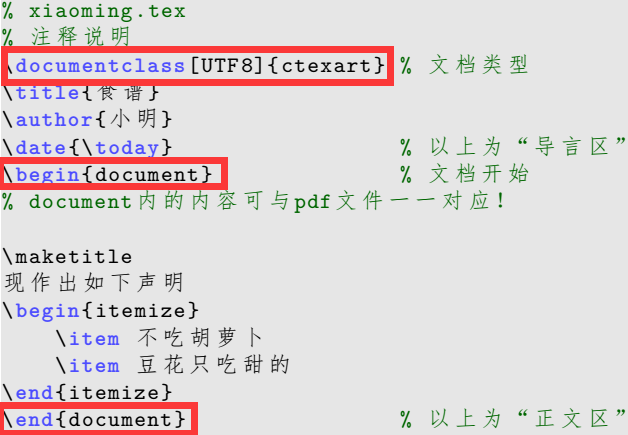
\includegraphics[width = 0.7\textwidth]{img//nece.png}
\end{figure}
    \end{frame}


\subsection{环境}
    \begin{frame}[fragile]
        \frametitle{什么是环境}
        \begin{itemize}
            \item 你也许注意到了\verb|\begin|和\verb|\end| \pause
            \item \verb|\begin|和\verb|\end|语句不是命令,而是对环境进行了定义。
            \item begin和end间的环境,代表这块区间应用的\textbf{排版}规则
            \item 可以多个环境层层嵌套(不可交叉!)
        \end{itemize}
    \end{frame}
    
    \begin{frame}[fragile]
\begin{lstlisting}
% 正确用法:

\begin{document}
  \begin{environment1}
    \begin{environment2}
    \end{environment2}
  \end{environment1}
\end{document}

% 错误用法:

\begin{document}
  \begin{environment1}
    \begin{environment2}
  \end{environment1}
    \end{environment2}
\end{document}
\end{lstlisting}
    \end{frame}
    
    
	\begin{frame}[fragile]
		\begin{itemize}
			\item 模块化与环境的思想\\
			打开 "environment\_cmp.tex"
			\item 为什么section2每一行都居中了?
			\item 你能不能通过添加环境的方式,让section2第一行靠左?(提示:flushleft)
			\item 这是否引发了你对优先级的思考?
		\end{itemize}
	\end{frame}
	
	
\subsection{字体}
    \begin{frame}
        \frametitle{问题}
        \begin{itemize}
            \item 字体太丑,或者有字体要求(如Times New Roman,俄语,德语)
            \item 字体颜色
            \item 键盘无法输入的符号(如$\pi$, \AA, $^{\circ}$C)
            \item 貌似可以用键盘输入的符号(如\%, \{, $\sim$)
            \item 其他(空格:\fbox{\$\qquad\$}, \fbox{\$\quad\$}, \fbox{\$\ \$}, \fbox{\$\;\$}, \fbox{\$~\$} \fbox{\$\,\$}, \fbox{\$\!\$})
        \end{itemize}
    \end{frame}

    \begin{frame}
        \frametitle{解决方法}
        \begin{itemize}
            \item 了解相关的宏包,以及相关命令设置,如fontspec,babel等等
            \item 要用去网上查
            \item 看手册(已准备好,在LM文件夹里)
            \item 以上两条也针对其他琐碎的细节,如字号、行距、盒子等等
        \end{itemize}
    \end{frame}
\section{文章结构}

\subsection{标题}
	\begin{frame}
		\begin{itemize}
			\item 打开 "title.tex"
			\item 通过添加和取消注释,看看前三种标题页的效果
			\item 主要是title,author,date(试试能不能在cetxart文档中使用subtitle)
			\item 自定义标题页
		\end{itemize}
	\end{frame}


\subsection{章节}
	\begin{frame}
		\begin{itemize}
			\item 打开 "tutorial to the freshmen of DII.pdf"
			\item 一篇完整的article或者report,其文本结构是怎样的?
		\end{itemize}
	\end{frame}
	
	\begin{frame}[fragile]
		\begin{itemize}
			\item 这篇report主要是中文内容,这种分模块(section),生成目录(tableofcontents)的形式,是一种十分经典的文章结构
			\item 这篇report主要用了以下几个命令(尝试寻找其他的章节命令,比如\verb|\clearpage vs \newpage|)
			\item 章节标题的格式是预定好的,一般需要用通过其他宏包完成定制(\verb|\CTEXset{}|)
			\item RTFM,查看CTEX宏集手册,尝试定义出“第一节”的章节标题编号
			\item 联想一下maketitle,document正文区里的代码是与pdf文件一一对应的,所以\verb|\tableofcontents|应该放在.tex文档的哪里?
			\item 通常主流的latex编辑器都能展示出你的各个section标题,尝试通过它更好地调整你的文章结构,或是快速定位代码
		\end{itemize}
	\end{frame}
	

\subsection{多文件编译}
	\begin{frame}
	    \frametitle{问题}
		\begin{itemize}
			\item 编译"tutorial to the freshmen of DII"需要多久?\pause
			\item 如果你要编译一整本书呢?\pause
			\item 与他人合作写一篇report或beamer等等,是否觉得各方整合起来会遇到很多问题?
		\end{itemize}\pause
	按文档的逻辑层次,把整个文档分成多个.tex源文件,便于检索管理以及多人协同编写
	\end{frame}
	
	\begin{frame}[fragile]
	    \frametitle{以讲座所用beamer为例}
	    \vspace{-3ex}
\begin{lstlisting}
%%%%%%%%%%%%%%%%%%%%%%%%%%%%%%%%%%%
% File: preamble.tex
%%%%%%%%%%%%%%%%%%%%%%%%%%%%%%%%%%%

\usepackage[top = 1.5cm]{geometry}

% Set fonts commands
\newcommand{\song}{\CJKfamily{song}} 
\newcommand{\hei}{\CJKfamily{hei}} 
\newcommand{\kai}{\CJKfamily{kai}} 
\newcommand{\fs}{\CJKfamily{fs}}

\newcommand{\me}[2]{\author{{\bfseries 姓名:}\underline{#1}\hspace{2em}{\bfseries 学号:}\underline{#2}}}

% Always keep this.
\newcommand{\noplagiarism}{
  \begin{center}
    \fbox{\begin{tabular}{@{}c@{}}
      请独立完成作业,不得抄袭。\\
      若参考了其它资料,请给出引用。\\
      鼓励讨论,但需独立书写解题过程。
    \end{tabular}}
  \end{center}
}

% Each hw consists of three parts:
% (1) this homework
\newcommand{\beginthishw}{\part{作业}}
% (2) corrections (Optional)
\newcommand{\begincorrection}{\part{订正}}
% (3) any feedback (Optional)
\newcommand{\beginfb}{\part{反馈}}

% For math
\usepackage{amsmath}
\usepackage{amsfonts}
\usepackage{amssymb}

% Define theorem-like environments
\usepackage[amsmath, thmmarks]{ntheorem}

\theoremstyle{break}
\theorembodyfont{\song}
\theoremseparator{}
\newtheorem*{problem}{题目}

\theorempreskip{2.0\topsep}
\theoremheaderfont{\kai\bfseries}
\theoremseparator{:}
% \newtheorem*{remark}{注}
\theorempostwork{\bigskip\hrule}
\newtheorem*{solution}{解答}
\theorempostwork{\bigskip\hrule}
\newtheorem*{revision}{订正}

\theoremstyle{plain}
\newtheorem*{cause}{错因分析}
\newtheorem*{remark}{注}

\theoremstyle{break}
\theorempostwork{\bigskip\hrule}
\theoremsymbol{\ensuremath{\Box}}
\newtheorem*{proof}{证明}

\renewcommand\figurename{图}
\renewcommand\tablename{表}

% For figures
% for fig with caption: #1: width/size; #2: fig file; #3: fig caption
\newcommand{\fig}[3]{
  \begin{figure}[htp]
    \centering
      \includegraphics[#1]{#2}
      \caption{#3}
  \end{figure}
}

% for fig without caption: #1: width/size; #2: fig file
\newcommand{\fignocaption}[2]{
  \begin{figure}[htp]
    \centering
    \includegraphics[#1]{#2}
  \end{figure}
}
\begin{document}
\frame{\titlepage}
\frame{\tableofcontents[hideallsubsections]}
\section{与\LaTeX 相遇}%hbk

\subsection{上手的准备}
\begin{frame}
    \frametitle{预防针}
    \begin{figure}
    \centering
    \begin{minipage}[t]{0.48\textwidth}
    \centering
    
\includegraphics[width=0.65\textwidth]{img//xieyi1.png}
    \end{minipage}
    \begin{minipage}[t]{0.48\textwidth}
    \centering
    
\includegraphics[width=0.65\textwidth]{img//xieyi2.png}
    \end{minipage}
    \end{figure}
\end{frame}

\begin{frame}
    \frametitle{怎样学习\LaTeX}
    本次讲座入门后,只需做到两点:
    \begin{itemize}
        \item STFW, Search the Friendly Web, 上网搜索
        \item RTFM, Read the Fuitful Manual, 看手册
    \end{itemize}
\end{frame}

\begin{frame}
    \frametitle{介绍}
    \LaTeX 是一种基于\TeX 的排版系统,即使用户没有排版和程序设计知识也可以生成优美的高质量的文档,其在复杂表格和数学公式上的表现尤其突出\\\pause
    \begin{center}
    精确\ \ 复杂\ \ 细节\ \ 品位
    \end{center}
    光说没用,举些例子——pre文件夹中两份平时作业\\\pause
    \text{LaTeX} 入门难,越用越方便;word 入门简单,越用越难
\end{frame}

\begin{frame}[fragile]
    \frametitle{上手试一试}
编译你的第一个.tex文件

\begin{lstlisting}
\documentclass{article}
   
\begin{document}
This is my first document\\
Hello, \LaTeX!
\end{document}
\end{lstlisting}

\end{frame}
\section{文档}

\subsection{框架}

    \begin{frame}[fragile]
        \begin{itemize}
            \item 你书写的是包含LaTeX代码和实际内容的纯文本文件(.tex文件)。
            \item LaTeX代码控制实际内容的格式和样式。
        \end{itemize}
    \end{frame}

	\begin{frame}[fragile]
\begin{lstlisting}
% xiaoming.tex
% 注释说明
\documentclass[UTF8]{ctexart} % 文档类型
\title{食谱}
\author{小明}
\date{\today}                 % 以上为“导言区”
\begin{document}              % 文档开始
% document内的内容可与pdf文件一一对应!
\maketitle
现作出如下声明
\begin{itemize}
    \item 不吃胡萝卜
    \item 豆花只吃甜的
\end{itemize}
\end{document}                % 以上为“正文区”
\end{lstlisting}
	\end{frame}


\subsection{两个必要元素}%hbk
	\begin{frame}[fragile]
	    \frametitle{documentclass}
		\begin{itemize}
			\item documenclass,文档类,是第一个必要元素:\\
			写的是什么,怎样排版
\begin{lstlisting}
\doucumentclass[·]{·}
% 方括号内为可选项,可设置纸张大小,字体大小,纸张方向,编码方式,草稿定稿,单双面等属性
\end{lstlisting}\pause
			\item 常用标准文档:\\
			article, book, report, letter, beamer (前三者为基本文档类;ctex宏集了解一下)
			\item cls文件:\\
			自定义的文档类型(CUMCMThesis-master)
		\end{itemize}
	\end{frame}
	
    \begin{frame}
        \frametitle{document}
        document环境是一份tex文档的第二个必要元素,其内为pdf文件的具体内容\pause
\begin{figure}
\centering
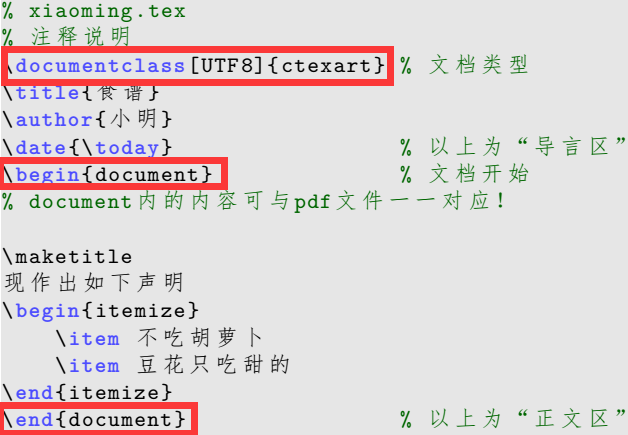
\includegraphics[width = 0.7\textwidth]{img//nece.png}
\end{figure}
    \end{frame}


\subsection{环境}
    \begin{frame}[fragile]
        \frametitle{什么是环境}
        \begin{itemize}
            \item 你也许注意到了\verb|\begin|和\verb|\end| \pause
            \item \verb|\begin|和\verb|\end|语句不是命令,而是对环境进行了定义。
            \item begin和end间的环境,代表这块区间应用的\textbf{排版}规则
            \item 可以多个环境层层嵌套(不可交叉!)
        \end{itemize}
    \end{frame}
    
    \begin{frame}[fragile]
\begin{lstlisting}
% 正确用法:

\begin{document}
  \begin{environment1}
    \begin{environment2}
    \end{environment2}
  \end{environment1}
\end{document}

% 错误用法:

\begin{document}
  \begin{environment1}
    \begin{environment2}
  \end{environment1}
    \end{environment2}
\end{document}
\end{lstlisting}
    \end{frame}
    
    
	\begin{frame}[fragile]
		\begin{itemize}
			\item 模块化与环境的思想\\
			打开 "environment\_cmp.tex"
			\item 为什么section2每一行都居中了?
			\item 你能不能通过添加环境的方式,让section2第一行靠左?(提示:flushleft)
			\item 这是否引发了你对优先级的思考?
		\end{itemize}
	\end{frame}
	
	
\subsection{字体}
    \begin{frame}
        \frametitle{问题}
        \begin{itemize}
            \item 字体太丑,或者有字体要求(如Times New Roman,俄语,德语)
            \item 字体颜色
            \item 键盘无法输入的符号(如$\pi$, \AA, $^{\circ}$C)
            \item 貌似可以用键盘输入的符号(如\%, \{, $\sim$)
            \item 其他(空格:\fbox{\$\qquad\$}, \fbox{\$\quad\$}, \fbox{\$\ \$}, \fbox{\$\;\$}, \fbox{\$~\$} \fbox{\$\,\$}, \fbox{\$\!\$})
        \end{itemize}
    \end{frame}

    \begin{frame}
        \frametitle{解决方法}
        \begin{itemize}
            \item 了解相关的宏包,以及相关命令设置,如fontspec,babel等等
            \item 要用去网上查
            \item 看手册(已准备好,在LM文件夹里)
            \item 以上两条也针对其他琐碎的细节,如字号、行距、盒子等等
        \end{itemize}
    \end{frame}
\section{文章结构}

\subsection{标题}
	\begin{frame}
		\begin{itemize}
			\item 打开 "title.tex"
			\item 通过添加和取消注释,看看前三种标题页的效果
			\item 主要是title,author,date(试试能不能在cetxart文档中使用subtitle)
			\item 自定义标题页
		\end{itemize}
	\end{frame}


\subsection{章节}
	\begin{frame}
		\begin{itemize}
			\item 打开 "tutorial to the freshmen of DII.pdf"
			\item 一篇完整的article或者report,其文本结构是怎样的?
		\end{itemize}
	\end{frame}
	
	\begin{frame}[fragile]
		\begin{itemize}
			\item 这篇report主要是中文内容,这种分模块(section),生成目录(tableofcontents)的形式,是一种十分经典的文章结构
			\item 这篇report主要用了以下几个命令(尝试寻找其他的章节命令,比如\verb|\clearpage vs \newpage|)
			\item 章节标题的格式是预定好的,一般需要用通过其他宏包完成定制(\verb|\CTEXset{}|)
			\item RTFM,查看CTEX宏集手册,尝试定义出“第一节”的章节标题编号
			\item 联想一下maketitle,document正文区里的代码是与pdf文件一一对应的,所以\verb|\tableofcontents|应该放在.tex文档的哪里?
			\item 通常主流的latex编辑器都能展示出你的各个section标题,尝试通过它更好地调整你的文章结构,或是快速定位代码
		\end{itemize}
	\end{frame}
	

\subsection{多文件编译}
	\begin{frame}
	    \frametitle{问题}
		\begin{itemize}
			\item 编译"tutorial to the freshmen of DII"需要多久?\pause
			\item 如果你要编译一整本书呢?\pause
			\item 与他人合作写一篇report或beamer等等,是否觉得各方整合起来会遇到很多问题?
		\end{itemize}\pause
	按文档的逻辑层次,把整个文档分成多个.tex源文件,便于检索管理以及多人协同编写
	\end{frame}
	
	\begin{frame}[fragile]
	    \frametitle{以讲座所用beamer为例}
	    \vspace{-3ex}
\begin{lstlisting}
%%%%%%%%%%%%%%%%%%%%%%%%%%%%%%%%%%%
% File: preamble.tex
%%%%%%%%%%%%%%%%%%%%%%%%%%%%%%%%%%%

\usepackage[top = 1.5cm]{geometry}

% Set fonts commands
\newcommand{\song}{\CJKfamily{song}} 
\newcommand{\hei}{\CJKfamily{hei}} 
\newcommand{\kai}{\CJKfamily{kai}} 
\newcommand{\fs}{\CJKfamily{fs}}

\newcommand{\me}[2]{\author{{\bfseries 姓名:}\underline{#1}\hspace{2em}{\bfseries 学号:}\underline{#2}}}

% Always keep this.
\newcommand{\noplagiarism}{
  \begin{center}
    \fbox{\begin{tabular}{@{}c@{}}
      请独立完成作业,不得抄袭。\\
      若参考了其它资料,请给出引用。\\
      鼓励讨论,但需独立书写解题过程。
    \end{tabular}}
  \end{center}
}

% Each hw consists of three parts:
% (1) this homework
\newcommand{\beginthishw}{\part{作业}}
% (2) corrections (Optional)
\newcommand{\begincorrection}{\part{订正}}
% (3) any feedback (Optional)
\newcommand{\beginfb}{\part{反馈}}

% For math
\usepackage{amsmath}
\usepackage{amsfonts}
\usepackage{amssymb}

% Define theorem-like environments
\usepackage[amsmath, thmmarks]{ntheorem}

\theoremstyle{break}
\theorembodyfont{\song}
\theoremseparator{}
\newtheorem*{problem}{题目}

\theorempreskip{2.0\topsep}
\theoremheaderfont{\kai\bfseries}
\theoremseparator{:}
% \newtheorem*{remark}{注}
\theorempostwork{\bigskip\hrule}
\newtheorem*{solution}{解答}
\theorempostwork{\bigskip\hrule}
\newtheorem*{revision}{订正}

\theoremstyle{plain}
\newtheorem*{cause}{错因分析}
\newtheorem*{remark}{注}

\theoremstyle{break}
\theorempostwork{\bigskip\hrule}
\theoremsymbol{\ensuremath{\Box}}
\newtheorem*{proof}{证明}

\renewcommand\figurename{图}
\renewcommand\tablename{表}

% For figures
% for fig with caption: #1: width/size; #2: fig file; #3: fig caption
\newcommand{\fig}[3]{
  \begin{figure}[htp]
    \centering
      \includegraphics[#1]{#2}
      \caption{#3}
  \end{figure}
}

% for fig without caption: #1: width/size; #2: fig file
\newcommand{\fignocaption}[2]{
  \begin{figure}[htp]
    \centering
    \includegraphics[#1]{#2}
  \end{figure}
}
\begin{document}
\frame{\titlepage}
\frame{\tableofcontents[hideallsubsections]}
\section{与\LaTeX 相遇}%hbk

\subsection{上手的准备}
\begin{frame}
    \frametitle{预防针}
    \begin{figure}
    \centering
    \begin{minipage}[t]{0.48\textwidth}
    \centering
    
\includegraphics[width=0.65\textwidth]{img//xieyi1.png}
    \end{minipage}
    \begin{minipage}[t]{0.48\textwidth}
    \centering
    
\includegraphics[width=0.65\textwidth]{img//xieyi2.png}
    \end{minipage}
    \end{figure}
\end{frame}

\begin{frame}
    \frametitle{怎样学习\LaTeX}
    本次讲座入门后,只需做到两点:
    \begin{itemize}
        \item STFW, Search the Friendly Web, 上网搜索
        \item RTFM, Read the Fuitful Manual, 看手册
    \end{itemize}
\end{frame}

\begin{frame}
    \frametitle{介绍}
    \LaTeX 是一种基于\TeX 的排版系统,即使用户没有排版和程序设计知识也可以生成优美的高质量的文档,其在复杂表格和数学公式上的表现尤其突出\\\pause
    \begin{center}
    精确\ \ 复杂\ \ 细节\ \ 品位
    \end{center}
    光说没用,举些例子——pre文件夹中两份平时作业\\\pause
    \text{LaTeX} 入门难,越用越方便;word 入门简单,越用越难
\end{frame}

\begin{frame}[fragile]
    \frametitle{上手试一试}
编译你的第一个.tex文件

\begin{lstlisting}
\documentclass{article}
   
\begin{document}
This is my first document\\
Hello, \LaTeX!
\end{document}
\end{lstlisting}

\end{frame}
\section{文档}

\subsection{框架}

    \begin{frame}[fragile]
        \begin{itemize}
            \item 你书写的是包含LaTeX代码和实际内容的纯文本文件(.tex文件)。
            \item LaTeX代码控制实际内容的格式和样式。
        \end{itemize}
    \end{frame}

	\begin{frame}[fragile]
\begin{lstlisting}
% xiaoming.tex
% 注释说明
\documentclass[UTF8]{ctexart} % 文档类型
\title{食谱}
\author{小明}
\date{\today}                 % 以上为“导言区”
\begin{document}              % 文档开始
% document内的内容可与pdf文件一一对应!
\maketitle
现作出如下声明
\begin{itemize}
    \item 不吃胡萝卜
    \item 豆花只吃甜的
\end{itemize}
\end{document}                % 以上为“正文区”
\end{lstlisting}
	\end{frame}


\subsection{两个必要元素}%hbk
	\begin{frame}[fragile]
	    \frametitle{documentclass}
		\begin{itemize}
			\item documenclass,文档类,是第一个必要元素:\\
			写的是什么,怎样排版
\begin{lstlisting}
\doucumentclass[·]{·}
% 方括号内为可选项,可设置纸张大小,字体大小,纸张方向,编码方式,草稿定稿,单双面等属性
\end{lstlisting}\pause
			\item 常用标准文档:\\
			article, book, report, letter, beamer (前三者为基本文档类;ctex宏集了解一下)
			\item cls文件:\\
			自定义的文档类型(CUMCMThesis-master)
		\end{itemize}
	\end{frame}
	
    \begin{frame}
        \frametitle{document}
        document环境是一份tex文档的第二个必要元素,其内为pdf文件的具体内容\pause
\begin{figure}
\centering
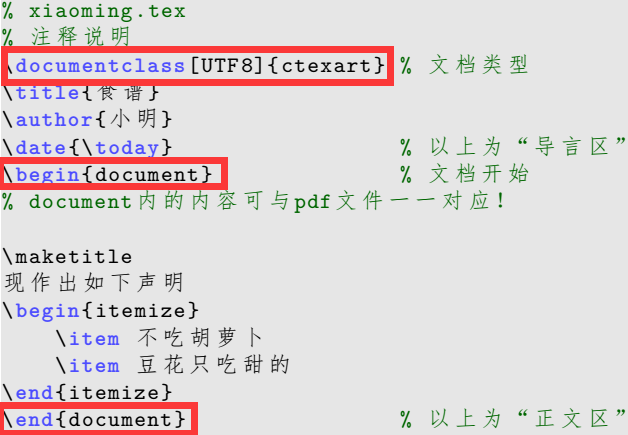
\includegraphics[width = 0.7\textwidth]{img//nece.png}
\end{figure}
    \end{frame}


\subsection{环境}
    \begin{frame}[fragile]
        \frametitle{什么是环境}
        \begin{itemize}
            \item 你也许注意到了\verb|\begin|和\verb|\end| \pause
            \item \verb|\begin|和\verb|\end|语句不是命令,而是对环境进行了定义。
            \item begin和end间的环境,代表这块区间应用的\textbf{排版}规则
            \item 可以多个环境层层嵌套(不可交叉!)
        \end{itemize}
    \end{frame}
    
    \begin{frame}[fragile]
\begin{lstlisting}
% 正确用法:

\begin{document}
  \begin{environment1}
    \begin{environment2}
    \end{environment2}
  \end{environment1}
\end{document}

% 错误用法:

\begin{document}
  \begin{environment1}
    \begin{environment2}
  \end{environment1}
    \end{environment2}
\end{document}
\end{lstlisting}
    \end{frame}
    
    
	\begin{frame}[fragile]
		\begin{itemize}
			\item 模块化与环境的思想\\
			打开 "environment\_cmp.tex"
			\item 为什么section2每一行都居中了?
			\item 你能不能通过添加环境的方式,让section2第一行靠左?(提示:flushleft)
			\item 这是否引发了你对优先级的思考?
		\end{itemize}
	\end{frame}
	
	
\subsection{字体}
    \begin{frame}
        \frametitle{问题}
        \begin{itemize}
            \item 字体太丑,或者有字体要求(如Times New Roman,俄语,德语)
            \item 字体颜色
            \item 键盘无法输入的符号(如$\pi$, \AA, $^{\circ}$C)
            \item 貌似可以用键盘输入的符号(如\%, \{, $\sim$)
            \item 其他(空格:\fbox{\$\qquad\$}, \fbox{\$\quad\$}, \fbox{\$\ \$}, \fbox{\$\;\$}, \fbox{\$~\$} \fbox{\$\,\$}, \fbox{\$\!\$})
        \end{itemize}
    \end{frame}

    \begin{frame}
        \frametitle{解决方法}
        \begin{itemize}
            \item 了解相关的宏包,以及相关命令设置,如fontspec,babel等等
            \item 要用去网上查
            \item 看手册(已准备好,在LM文件夹里)
            \item 以上两条也针对其他琐碎的细节,如字号、行距、盒子等等
        \end{itemize}
    \end{frame}
\section{文章结构}

\subsection{标题}
	\begin{frame}
		\begin{itemize}
			\item 打开 "title.tex"
			\item 通过添加和取消注释,看看前三种标题页的效果
			\item 主要是title,author,date(试试能不能在cetxart文档中使用subtitle)
			\item 自定义标题页
		\end{itemize}
	\end{frame}


\subsection{章节}
	\begin{frame}
		\begin{itemize}
			\item 打开 "tutorial to the freshmen of DII.pdf"
			\item 一篇完整的article或者report,其文本结构是怎样的?
		\end{itemize}
	\end{frame}
	
	\begin{frame}[fragile]
		\begin{itemize}
			\item 这篇report主要是中文内容,这种分模块(section),生成目录(tableofcontents)的形式,是一种十分经典的文章结构
			\item 这篇report主要用了以下几个命令(尝试寻找其他的章节命令,比如\verb|\clearpage vs \newpage|)
			\item 章节标题的格式是预定好的,一般需要用通过其他宏包完成定制(\verb|\CTEXset{}|)
			\item RTFM,查看CTEX宏集手册,尝试定义出“第一节”的章节标题编号
			\item 联想一下maketitle,document正文区里的代码是与pdf文件一一对应的,所以\verb|\tableofcontents|应该放在.tex文档的哪里?
			\item 通常主流的latex编辑器都能展示出你的各个section标题,尝试通过它更好地调整你的文章结构,或是快速定位代码
		\end{itemize}
	\end{frame}
	

\subsection{多文件编译}
	\begin{frame}
	    \frametitle{问题}
		\begin{itemize}
			\item 编译"tutorial to the freshmen of DII"需要多久?\pause
			\item 如果你要编译一整本书呢?\pause
			\item 与他人合作写一篇report或beamer等等,是否觉得各方整合起来会遇到很多问题?
		\end{itemize}\pause
	按文档的逻辑层次,把整个文档分成多个.tex源文件,便于检索管理以及多人协同编写
	\end{frame}
	
	\begin{frame}[fragile]
	    \frametitle{以讲座所用beamer为例}
	    \vspace{-3ex}
\begin{lstlisting}
\input{part/preamble}
\begin{document}
\frame{\titlepage}
\frame{\tableofcontents[hideallsubsections]}
\input{part/try}
\input{part/docu}
\input{part/stru}
\input{part/textenvi}
\input{part/chin}
\input{part/formula}
\input{part/tab&fig}
\input{part/slides}
\input{part/auto}
\input{part/others}
\end{document}
\end{lstlisting}
	\end{frame}

	\begin{frame}[fragile]
		\indent 划分文档的主要方式是\verb|\input{}|和\verb|\include{}|,将不同的章节内容写在不同的.tex文件中,用上述两种方式引入主文件中。\\
		\begin{description}
			\item[input] 相当于ctrl+c和ctrl+v,直接把代码复制过来,稳定、实用
			\item[include] 常和\verb|\includeonly|一起使用,可以选择性地编译子文件,常用于书籍之类的特大文档
		\end{description}
		\indent 两种方式的编译效果有细节上的不同,自己试试
	\end{frame}

	\begin{frame}
	截图来自stackexchange.com,题为input vs include
	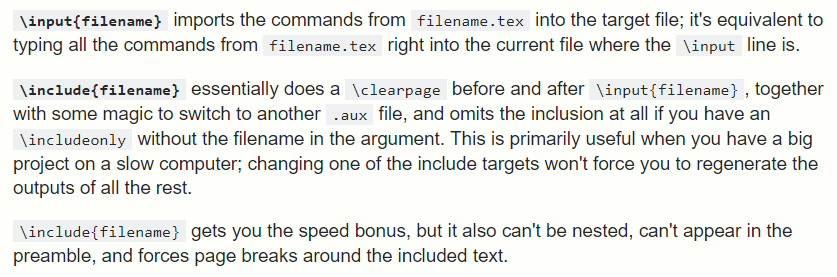
\includegraphics[width=\textwidth]{img//vs.png}	
	\end{frame}

	\begin{frame}[fragile]
		我们用的比较多的是input,当你觉得某一部分代码太长时,可以考虑写在别的.tex文件中,精简主文件,平时主要用在下面几种情况
		\begin{itemize}
			\item 导言区繁多的设置(通常会写在名为preamble的文件中,请看问求的作业模板)
			\item 异常庞大的表格
			\item 设置复杂的图片(比如需要使用很多子图subfig时)
		\end{itemize}
		此外可以去了解一下\verb|\endinput|的使用
	\end{frame}

\section{文本环境举隅}

\subsection{常用文本环境}

    \begin{frame}
    (其实会下面的就够了……)
    \begin{itemize}
        \item 文本环境:quote, quotation, abstarct(写诗的同学可以去了解verse)
        \item 列表环境:itemize, enumerate
        \item 定理类环境:thm, lemma, definition, proof
        \item 抄录和代码环境:verb, lstlisting
        \item 脚注:footnote
    \end{itemize}
    \end{frame}
    
    \begin{frame}
    \frametitle{练习和小建议}
    \begin{itemize}
    \item 打开练习list, theorem, listing$\_$code, page
    \item 想要用好文本环境,更建议看手册而不是上网搜索
    \end{itemize}
    \end{frame}
\section{中文支持}
\subsection{了解\CTeX}
\begin{frame}{How to get Chinese document?}{\CTeX}
	\CTeX 是最新的也是最便利的\LaTeX 中文支持的开源项目,可以参考其\href{material/LM/CTEXmanual.pdf}{\textcolor{blue}{使用手册}}。
	\begin{itemize}
		\item 全面汉化
		\item 更智能的排版
		\item 强大的自定义设置
	\end{itemize}
	一般使用默认设置即可,有特殊需求可翻阅手册作适当调整。
\end{frame}
\begin{frame}
	\begin{table}\caption{\CTeX 宏集的组成}
		\footnotesize
		\begin{tabular}{llp{6cm}}
			\toprule
			类别 & 文件 & 说明 \\
			\midrule
			文档类 & ctexart.cls & 标准文档类article 的汉化版本,一般适用于短篇幅的文章\\
			& ctexrep.cls & 标准文档类report 的汉化版本,一般适用于中篇幅的报告\\
			& ctexbook.cls & 标准文档类book 的汉化版本,一般适用于长篇幅的书籍\\
			& ctexbeamer.cls & 文档类beamer 的汉化版本,适用于幻灯片演示\\
			\midrule
			宏包 & ctex.sty & 提供全部功能,但默认不开启章节标题设置功能,需要使用heading 选项来开启\\
			& ctexsize.sty & 定义和调整中文字号,在ctex 宏包或CTEX 中文文档类之外单独调用\\
			& ctexheading.sty & 提供章节标题设置功能,在ctex 宏包或CTEX 中文文档类之外单独调用\\
			\bottomrule
		\end{tabular}
	\end{table}
\end{frame}
\begin{frame}[fragile]
	\begin{itemize}
		\item 文档类
\begin{lstlisting}
\documentclass{ctexart}
\documentclass{ctexrep}
\documentclass{ctexbook}
\documentclass{ctexbeamer}
\end{lstlisting}		
		\item 宏包
\begin{lstlisting}
\usepackage{ctex}
\usepackage{ctexsize}      
\usepackage{ctexheading}   
\end{lstlisting}
	\end{itemize}
	\vspace{2ex}
	\textcolor{red}{注意}:\texttt{ctexcap} 是默认打开 \texttt{heading} 选项的 \texttt{ctex} 宏包,手册中明确说明其为过时宏包!
\end{frame}
\begin{frame}
	两个最常用选项\texttt{heading}与\texttt{scheme}。

	打开\texttt{ctex.tex},体会不同选项的区别。
	\begin{itemize}
		\item \texttt{ctexart}类文档与\texttt{ctex}宏包的默认选项都是\texttt{heading=true,scheme=chinese}
		\item \texttt{heading=false,scheme=plain}相当于只是支持中文,所有的版式都还是英文的
		\item 如果觉得标题居中太蠢了想要靠左,可以用\texttt{heading=false}(\texttt{scheme=chinese}是默认选项不用改)
	\end{itemize}
\end{frame}
\section{强大的数学公式}
\begin{frame}[fragile]{写在前面}
	除了一些最简单的数学公式,大部分都需要宏包支持。建议平时需要输入公式时就直接使用以下四个宏包
\begin{lstlisting}
\usepackage{amsmath,amsfonts,amssymb,mathtools}
\end{lstlisting}
	这能够支持大多数的数学公式,而不必去纠结什么时候应该用哪一个、哪一个是多余的。

	\vspace{2ex}
	在讨论更多的数学环境前,我们统一使用 \cprotect\fbox{\verb|$|$\dots$\verb|$|} 输入行内(inline)公式,\cprotect\fbox{\verb|\[|$\dots$\verb|\]|} 输入行间(displayed)公式。

	\vspace{2ex}
	\textcolor{red}{注意}:凡是要用到数学字符的地方必须进入数学环境,有些字符虽然不在数学环境下也能输入,但是区别很大!
	\begin{table}
		\begin{tabular}{rlrl}
			\textrm{1+1=2} & $1+1=2$ \quad & \quad \textrm{a sin x} & $a \sin x$
		\end{tabular}
	\end{table}
\end{frame}

\subsection{数学符号}
\begin{frame}[fragile]{字母表与数学字体}
	在公式环境内默认使用 \cprotect\fbox{\verb|\mathnormal|} 字体,与正文环境下默认字体对比如下
	\begin{itemize}
		\item Capital
		\begin{itemize}
			\item \textrm{ABCDEFGHIJKLMNOPQRSTUVWXYZ}
			\item $ABCDEFGHIJKLMNOPQRSTUVWXYZ$
		\end{itemize}
		\item Lower case
		\begin{itemize}
			\item \textrm{abcdefghijklmnopqrstuvwxyz}
			\item $abcdefghijklmnopqrstuvwxyz$
		\end{itemize}
	\end{itemize}
	其明显特征是斜体且间距较正文大一些。

	\vspace{2ex}
	而\cprotect\fbox{\verb|\mathit|}, \cprotect\fbox{\verb|\mathrm|}, \cprotect\fbox{\verb|\mathbf|}, \cprotect\fbox{\verb|\mathsf|}, \cprotect\fbox{\verb|\mathtt|} 这些数学字体通常直接使用相对应的正文字体\cprotect\fbox{\verb|\text**|}。
\end{frame}
\begin{frame}[fragile]{选用正确的字体}
	\begin{itemize}
		\item 变量使用默认字体,如$x, y, z$
		\item $\mathrm{e}, \mathrm{i}$等常量应使用罗马体 \cprotect\fbox{\verb|\mathrm|}
		\item 集合$\mathbb{N}, \mathbb{R}$等可使用 \verb|amssymb|提供的黑板粗体 \cprotect\fbox{\verb|\mathbb|}
		\item 向量$\bm{v}$应加粗,实现方法有很多,这里推荐 \verb|bm| 宏包的 \cprotect\fbox{\verb|\bm|} 命令
	\end{itemize}
\end{frame}
\begin{frame}[fragile]{希腊字母}
	\begin{itemize}
		\item 小写希腊字母
		\begin{itemize}
			\item 一般 \cprotect\fbox{\verb|\+小写拼写|},如 \cprotect\fbox{\verb|\alpha|} 即输出$\alpha$
			\item 注意$\mu, \nu$分别为 \cprotect\fbox{\verb|\mu|},\cprotect\fbox{\verb|\nu|}
			\item 一部分希腊字母有变体,这些变体在数学公式中常常用到,只需在前面加上 \verb|var|
				\begin{itemize}
				\item[] \small $\epsilon \rightarrow \varepsilon$ \qquad $\phi \rightarrow \varphi$ \qquad
					$\theta \rightarrow \vartheta$ \qquad $\sigma \rightarrow \varsigma$ \qquad
					$\pi \rightarrow \varpi$
				\end{itemize}
		\end{itemize}
		\item 大写希腊字母
		\begin{itemize}
			\item 一部分大写希腊字母与拉丁字母形状相同,直接使用即可,如$\mathrm{A, B}$
			\item 将小写希腊字母输入时首字母大写即可得到其大写形式,如 \cprotect\fbox{\verb|\Gamma|} 得到$\Gamma$
			\item 大写希腊字母一般用正体,前面加 \cprotect\fbox{\verb|var|} 或使用 \cprotect\fbox{\verb|\mathnormal|} 可得到倾斜形式
		\end{itemize}
		\item 小写希腊字母直立体形式?
		\begin{itemize}
			\item 数字字体宏包 \verb|upgreek|,在前面加上 \cprotect\fbox{\verb|up|}
			\item \cprotect\fbox{\verb|\pi|} $\rightarrow$ \cprotect\fbox{\verb|\uppi|} \qquad $\pi \rightarrow \uppi$
		\end{itemize}
	\end{itemize}
\end{frame}
\begin{frame}[fragile]{常用符号}
	\begin{table}\caption{数学普通符号(部分)}
		\begin{tabular}{llllll}
			\toprule
			$\hbar$ & \verb|\hbar| & $\ell$ & \verb|\ell| & $\partial$ & \verb|\partial| \\
			$\infty$ & \verb|\infty| & $\prime$ & \verb|\prime| & $\emptyset$ & \verb|\emptyset| \\
			$\nabla$ & \verb|\nabla| & $\forall$ & \verb|\forall| & $\exists$ & \verb|exists| \\
			$\neg$ & \verb|\neg| & $\varnothing$ & \verb|\varnothing| & $\angle$ & \verb|\angle| \\
			$\clubsuit$ & \verb|\clubsuit| & $\diamondsuit$ & \verb|\diamondsuit| & $\heartsuit$ & \verb|\heartsuit| \\
			$\spadesuit$ & \verb|\spadesuit| & $\triangle$ & \verb|\triangle| & $\square$ & \verb|\square| \\
			$\flat$ & \verb|\flat| & $\natural$ & \verb|\natural| & $\sharp$ & \verb|\sharp|\\
			\bottomrule
		\end{tabular}
	\end{table}
\end{frame}
\begin{frame}[fragile]{常用符号}
	\begin{table}\caption{可同时用在文本和数学模式中的符号}
		\begin{tabular}{llllllll}
			\toprule
			$\#$ & \verb|\#| & $\&$ & \verb|\&| & $\%$ & \verb|\%| & $\$$ & \verb|\$| \\
			$\_$ & \verb|\_| & $\{$ & \verb|\{| & $\}$ & \verb|\}| & & \\
			$\P$ & \verb|\P| & $\S$ & \verb|\S| & $\dag$ & \verb|\dag| & $\ddag$ & \verb|\ddag| \\
			$\copyright$ & \verb|\copyright| & $\pounds$ & \verb|\pounds| & $\ldots$ & \verb|\ldots| & & \\
			$\checkmark$ & \verb|\checkmark| & $\circledR$ & \verb|\circledR| & $\maltese$ & \verb|\maltese| & $\yen$ & \verb|\yen| \\
			\bottomrule
		\end{tabular}
	\end{table}
	\begin{table}\caption{希伯来字母}
		\begin{tabular}{llllllll}
			\toprule
			$\aleph$ & \verb|\aleph| & $\beth$ & \verb|\beth| & $\daleth$ & \verb|\daleth| & $\gimel$ & \verb|\gimel| \\
			\bottomrule
		\end{tabular}
	\end{table}
\end{frame}
\begin{frame}[fragile]{数学算子}{Math operator}
	\begin{itemize}
		\item 巨算符(large operator)
		\begin{itemize}
			\item 所谓巨算符是大小可变的运算符
			\item 其在行内与行间大小是不同的
			\item 一般可以添加有上下标(数学结构中会讲)
			\item 行内行间上下标的形式也有所不同
		\end{itemize}
	\end{itemize}
	\begin{align*}
		\int_a^b & \textstyle \int_a^b & \iint_m^n & \textstyle \iint_m^n & \oint_{|z|=1} & \textstyle \oint_{|z|=1} \\
		\sum_{n=0}^{\infty} & \textstyle \sum_{n=0}^{\infty} & \prod_{1 \le i < j \le n} & \textstyle \prod_{1 \le i < j \le n} & \bigcup\nolimits_{i=1}^{n} & \textstyle \bigcup\limits_{i=1}^{n}
	\end{align*}
	\small \quad \cprotect\fbox{\verb|\limits|} \quad \cprotect\fbox{\verb|\nolimits|} \quad 行内公式尽量避免上下限放在算符上下位置
\end{frame}
\begin{frame}[fragile]{数学算子}{Math operator}
	\begin{itemize}
		\item 文字名称的算子
		\begin{itemize}
			\item 使用直立罗马体排印,一般 \cprotect\fbox{\verb|\+名称|} 即可
			\item 分为两类,带上下限的与不带上下限的
			\begin{itemize}
				\item $\log \quad \sin \quad \cosh \quad \arctan \quad \exp$ 
				\item $\lim \quad \max \quad \min \quad \sup \quad \inf$ 
			\end{itemize}
			\item 带上下限的算子使用起来与巨算符相似\\
				\qquad $\lim\limits_{x \to 0} \qquad \lim_{x \to 0}$
			\item 如果需要定义新的算子,可以在导言区使用 \verb|\DeclareMathOperator(*)|,带 \verb|*|表示带上下限
			\begin{itemize}
				\item \verb|\DeclareMathOperator{\arccot}{arccot}| \\ $\arccot$
				\item \verb|\DeclareMathOperator{\sign}{sgn}| \\ $\sign$
				\item \verb|\DeclareMathOperator*{\limsup}{lim\,sup}| \\ $\limsup$
			\end{itemize}
		\end{itemize}
	\end{itemize}
\end{frame}
\begin{frame}[fragile]{二元运算符与关系符}
	\begin{itemize}
		\item $\cprotect\overset{\cprotect\fbox{\scriptsize\verb|+|}}{+}, 
	\cprotect\underset{\cprotect\fbox{\scriptsize\verb|-|}}{-}, 
	\cprotect\overset{\cprotect\fbox{\scriptsize\verb|\times|}}{\times}, 
	\cprotect\underset{\cprotect\fbox{\scriptsize\verb|\div|}}{\div}$等二元运算符与
	$\cprotect\overset{\cprotect\fbox{\scriptsize\verb|=|}}{=}, 
	\cprotect\underset{\cprotect\fbox{\scriptsize\verb|>|}}{>}, 
	\cprotect\overset{\cprotect\fbox{\scriptsize\verb|<|}}{<}, 
	\cprotect\underset{\cprotect\fbox{\scriptsize\verb|\ne|}}{\ne}, 
	\cprotect\overset{\cprotect\fbox{\scriptsize\verb|\le|}}{\le}$\textrm{,} $
	\cprotect\underset{\cprotect\fbox{\scriptsize\verb|\ge|}}{\ge}$\textrm{,} $
	\cprotect\overset{\cprotect\fbox{\scriptsize\verb|\ll|}}{\ll}$\textrm{,} $
	\cprotect\underset{\cprotect\fbox{\scriptsize\verb|\gg|}}{\gg}$等关系符与前后变量之间会保留一定的空隙,且行内公式可以在它们的后面断行。
	\item 二元关系符数量庞大,除了一些最常用的,一般有需要的时候随用随查即可。
	\item 使用 \cprotect\fbox{\verb|\mathbin|} 和 \cprotect\fbox{\verb|\mathrel|} 可以将其参数当作二元运算符和二元关系符来对待,可用于定义新运算或一些其他用途。
	\item 箭头符号与逻辑符号使用时同样可以查阅,不再赘述。
	\end{itemize}
\end{frame}
\begin{frame}[fragile]{定界符}
	\[\{\frac{\partial y_j}{\partial x_i} | i=1,2,\cdots,n,\, j=1,2,\cdots,m\}\]
	\[\left\{\frac{\partial y_j}{\partial x_i} \middle| i=1,2,\cdots,n,\, j=1,2,\cdots,m\right\}\]
	上例中的$\{\,|\,\}$均为定界符,其大小可以根据式子的大小而改变。
	\begin{itemize}
		\item 括号定界符
		\[(\,)\quad[\,]\quad\{\,\}\quad\langle\,\rangle\quad\lfloor\,\rfloor\quad\lceil\,\rceil\]
		\item 非括号定界符
		\[/\quad\backslash\quad|\quad\|\]
		\item 输入
		\begin{itemize}
			\item \verb|( ) [ ] \{ \} \langle \rangle|\\
				\verb|\lfloor \rfloor \lceil \rceil|
			\item \verb!/ \backslash | \|!
		\end{itemize}
	\end{itemize}
\end{frame}
\begin{frame}[fragile]{如何确定定界符大小}
	\begin{itemize}
		\item 自动调整
		\begin{itemize}
			\item 使用 \cprotect\fbox{\verb|\left( ... \right)|},左右必须成对出现
			\item 如果只需要一个定界符,可以用 \cprotect\fbox{\verb|.|} 表示空的定界符,如 \cprotect\fbox{\verb|\left.|}
			\item 需要三个定界符的话可使用 \cprotect\fbox{\verb|\middle|} 放在中间,如前例
		\end{itemize}
		\item 手动调整
		\begin{itemize}
			\item 提供了 \cprotect\fbox{\verb|\big|},\cprotect\fbox{\verb|\Big|}, \cprotect\fbox{\verb|\bigg|},\cprotect\fbox{\verb|\Bigg|} 四种大小供手动调节
			\item 可以在后面加上 \cprotect\fbox{\verb|l m r|} 配套使用
			\item 自动调整效果不理想时,可以试试手动调整
			\item 在明确“左右”(如 \cprotect\fbox{\verb|\left \right|} 或 \cprotect\fbox{\verb|\Bigl \Bigr|})时,可直接使用 \cprotect\fbox{\verb|<>|} 表示尖括号而不致与$<>$混淆
		\end{itemize}
	\end{itemize}
\end{frame}
\begin{frame}[fragile]{标点符号}
	\begin{itemize}
		\item 数学环境内应使用英文标点,否则会报错
		\item 常用的标点符号有$, \quad ; \quad ! \quad ? \quad \colon$
		\item 应注意的是\cprotect\fbox{\verb|:|}是作为二元关系符存在的(如$f(x):=x, \{x : x>0\}$),而作为标点的冒号是 \cprotect\fbox{\verb|\colon|},其两侧间距不同,表示比例时则最好用 \cprotect\fbox{\verb|\mathbin{:}|}
		\item 省略号有很多种,在矩阵中常用到,平时最常用的是 \cprotect\fbox{\verb|\cdots|} $\cdots$ 和 \cprotect\fbox{\verb|\ldots|} $\ldots$ (或直接使用 \cprotect\fbox{\verb|\dots|} 让latex自己选择)
		\item 标点后是无法换行的,像$f(x,y,z)$谁也不希望在中间断行,而$a_1$\textrm{,} $a_2$\textrm{,} $a_3$\textrm{,} $\cdots$\textrm{,} $a_n$希望能断行时应将标点置于数学环境之外并加上空格
		\item 数学环境中空格不起作用,但可以分隔各部分让公式结构更清晰
	\end{itemize}
\end{frame}

\subsection{数学结构}
\begin{frame}[fragile]{上下标}
	\begin{itemize}
		\item 上标用 \verb|^| 表示,下标用 \verb|_| 表示
		\item 超过一个字符时就应使用$\{\,\}$
		\item \verb|'| 是一种特殊的上标,相当于 \cprotect\fbox{\verb|^\prime|}
		\item 使用 \cprotect\fbox{\verb|\overset|} 和 \cprotect\fbox{\verb|\underset|}可以在任意符号上下方添加标记
	\end{itemize}
\end{frame}
\begin{frame}[fragile]{分式}
	\begin{itemize}
		\item 使用 \cprotect\fbox{\verb|\frac{num}{den}|} 输入分式,先输入分子(numerator),后输入分母(denominator)
		\item 行内默认使用正文格式(text style)分式,行间默认使用显示格式(display style)分式,可以使用 \cprotect\fbox{\verb|\tfrac|} 与 \cprotect\fbox{\verb|\dfrac|} 指定使用某一种
		\item 行内使用分式时,$a/b$效果往往比$\frac ab$更好
		\item 连分式用 \cprotect\fbox{\verb|\cfrac|},这里不细讲
		\item 顺带一提,\cprotect\fbox{\verb|\textstyle|} 和 \cprotect\fbox{\verb|\displaystyle|} 可以指定整条公式以哪种方式显示
	\end{itemize}
\end{frame}
\begin{frame}[fragile]{根式}
	\begin{itemize}
		\item \cprotect\fbox{\verb|\sqrt[root]{arg}|}
		\item \texttt{[\,]}内为可选项,用\cprotect\fbox{\verb|\uproot|} 与 \cprotect\fbox{\verb|\leftroot|} 可以微调\texttt{root}位置,参数为整数
		\item 被开方数不是整数或结构复杂时,通常改用等价的指数形式
		\item 使用 \cprotect\fbox{\verb|\vphantom|} 占位来获得统一的高度\\[1ex]
		\verb|\sqrt{\frac 12} < \sqrt{\vphantom{\frac12}2}|
		\[\sqrt{\frac 12} < \sqrt{\vphantom{\frac12}2}\]
		\item \cprotect\fbox{\verb|\mathstrut|} 用来平衡不同高度和深度的字母\\[1ex]
		\verb|\sqrt b \sqrt y|\\
		\verb|\sqrt{\mathstrut b} \sqrt{\mathstrut y}|
		\[\sqrt b \sqrt y \quad \rightarrow \quad \sqrt{\mathstrut b} \sqrt{\mathstrut y}\]
	\end{itemize}
\end{frame}
\begin{frame}[fragile]{矩阵}
	\begin{itemize}
		\item 输入矩阵结构需要矩阵环境,它们的区别在于外面的括号不同
		\begin{itemize}
			\item \texttt{ matrix}环境 \quad 无括号
			\item \texttt{pmatrix}环境 \quad 圆括号
			\item \texttt{bmatrix}环境 \quad 方括号
			\item \texttt{Bmatrix}环境 \quad 大括号
			\item \texttt{vmatrix}环境 \quad 单竖线
			\item \texttt{Vmatrix}环境 \quad 双数线
		\end{itemize}
		\item 以一个最简单的二阶矩阵为例\\
		\begin{minipage}[c]{0.5\textwidth}
\begin{lstlisting}
\[ \begin{pmatrix}
       a_{11} & a_{12} \\
       a_{21} & a_{22}
   \end{pmatrix} \]
\end{lstlisting}
		\end{minipage}
		\begin{minipage}[c]{0.4\textwidth}
			\[ \begin{pmatrix}
				a_{11} & a_{12} \\
				a_{21} & a_{22}
			\end{pmatrix} \]
		\end{minipage}
	\end{itemize}
\end{frame}
\subsection{数学环境}
\begin{frame}[fragile]{概述}
	我们先前使用的 \cprotect\fbox{\verb|\[|$\dots$\verb|\]|} 实质是
\begin{lstlisting}
\begin{equation*}
    ...
\end{equation*}
\end{lstlisting}
	的缩写,其中“$*$”表示不给该公式标序。

	\vspace{2ex}
	出于各方面的需求,我们并不满足于这样一个简单居中、无法换行的数学环境,而是会有诸多其他方面的要求。这时我们需要更多的数学环境来提供支持。
\end{frame}
\begin{frame}[fragile]{多行公式}{每行均为一个公式}
	\begin{itemize}
		\item 简单的多个公式罗列: \verb|gather(*)|
		\begin{itemize}
			\item 每行公式都是居中显示的
			\item 使用 \cprotect\fbox{\verb|\\|} 换行
			\item 某行不需要编号,在 \cprotect\fbox{\verb|\\|} 前加  \cprotect\fbox{\verb|\notag|} 
		\end{itemize}
		\item 公式按关系符对齐: \verb|align(*)|
		\begin{itemize}
			\item 使用 \cprotect\fbox{\verb|\\|} 换行,关系符前加 \cprotect\fbox{\verb|&|} 表示对齐
			\item \cprotect\fbox{\verb|&|} 一般放在二元关系符($=,<,>$等)前面
			\item 有时可巧用 \cprotect\fbox{\verb|\phantom|} 变通 
		\end{itemize}
		\item 多行公式每行都会产生一个编号,不希望产生的话可以使用\cprotect\fbox{\verb|\notag|}
	\end{itemize}
\end{frame}
\begin{frame}
	练习:尝试输出以下公式。

	\begin{minipage}{0.95\textwidth}
	\begin{gather}
		\partialratio{A}{x}{y} = \lim_{\Delta x \to 0} \frac{f(x+\varDelta x,y)-f(x,y)}{\varDelta x} \\
		\partialratio{A}{y}{x} = \lim_{\Delta y \to 0} \frac{f(x,y+\varDelta y)-f(x,y)}{\varDelta y}
	\end{gather}
	\hrule
	\begin{align}
		& \mathrel{\phantom{=}} (a + b)(a^2 - ab + b^2)\notag \\
		& = a^3 - a^2b + ab^2 + a^2b - ab^2 + b^3\notag \\
		& = a^3 + b^3
	\end{align}
	\end{minipage}
\end{frame}
\begin{frame}[fragile]{多行公式}
	\begin{itemize}
		\item \verb|align(*)| 的另一个用处:排版多列公式
		\begin{itemize}
			\item 每行的基本格式
			\begin{itemize}
				\item[] \verb|a &= b  &  c &= d  &  e &= f \\|
			\end{itemize}
			\item 最后一行不需要 \cprotect\fbox{\verb|\\|}
			\item 按照行来标序
			\item \cprotect\fbox{\verb|&|} 必然为奇数个,出现偶数个会报错(为什么?)
		\end{itemize}
		\item 关于 \verb|flalign(*)|
		\begin{itemize}
			\item 与 \verb|align(*)| 是类似的
			\item 会把多列公式水平方向分散对齐
		\end{itemize}
		\item 关于 \verb|alignat(*)|
		\begin{itemize}
			\item 与 \verb|align(*)| 也是类似的
			\item 不会主动产生间距,需要手动输入间距大小
			\item 需要一个参数表示每行要对齐的公式个数
		\end{itemize}
	\end{itemize}
\end{frame}
\begin{frame}[fragile]
	对比 \verb|align(*)| 与 \verb|flalign(*)|

	\vspace{2ex}
	\clean
	\begin{minipage}{0.49\textwidth}
		\begin{itemize}
			\item 使用 \verb|align|
			\begin{align}
				x + y &= 2 & x &= 1 \\
				x - y &= 0 & y &= 1
			\end{align}
		\end{itemize}
	\end{minipage}
	\clean
	\begin{minipage}{0.49\textwidth}
		\begin{itemize}
			\item 使用 \verb|flalign|
			\begin{flalign}
				x + y &= 2 & x &= 1 \\
				x - y &= 0 & y &= 1
			\end{flalign}
		\end{itemize}
	\end{minipage}

	\vspace{3ex}
	巧用 \verb|alignat|(使用 \verb|align|必须借助 \cprotect\fbox{\verb|\phantom|})

	\begin{minipage}{0.69\textwidth}
\begin{lstlisting}
\begin{alignat*}{5}
    &1 & &+2 & &+3 & &+4 & &=10 \\
    &1 & &   & &+3 & &   & &=4 \\
    &  & &+2 & &   & &+4 & &=6
\end{alignat*}
\end{lstlisting}			
	\end{minipage}
	\begin{minipage}{0.29\textwidth}
		\begin{alignat*}{5}
			&1 & &+2 & &+3 & &+4 & &=10 \\
			&1 & &   & &+3 & &   & &=4 \\
			&  & &+2 & &   & &+4 & &=6
		\end{alignat*}
	\end{minipage}
\end{frame}
\begin{frame}[fragile]{多行公式}
	\begin{itemize}
		\item 如何在多行公式之间插入说明性文字?
		\begin{itemize}
			\item 每次都退出数学环境输入文字过于麻烦
			\item 退出数学环境会破环上下公式间对齐关系
		\end{itemize}
		\item \cprotect\fbox{\verb|\text|} 行内插入文字
		\item \cprotect\fbox{\verb|\intertext|} 换行顶格插入文字(前一行的 \cprotect\fbox{\verb|\\|} 可省略)
		\item \cprotect\fbox{\verb|\shortintertext|} 提供更为紧凑的行间距
	\end{itemize}
\end{frame}
\begin{frame}
	例:

	\vspace{2ex} \clean
	绝热过程中,$Q=0$,不做非膨胀功时,有
	\begin{gather}
		\di U = \delta W
		\quad \text{或} \quad
		\di U + p \di V = 0
		\shortintertext{已知}
		\todi{U}{T}{V}
		\shortintertext{对理想气体,}
		\di U = C_V \di T, \quad \Delta U = \int_{T_1}^{T_2}C_V \di T
		\intertext{若$C_V$为常数,}
		\Delta U = C_V(T_2-T_1) = W
	\end{gather}
\end{frame}
\begin{frame}[fragile]{多行公式}
	\begin{itemize}
		\item 多个联系紧密的公式如何共用一个编号?
		\begin{itemize}
			\item[] 使用 \verb|subequations| 环境
		\end{itemize}
		\item 示例:
\begin{lstlisting}
\begin{subequations}
\begin{align}
  a \cdot b &= b \cdot a \\
  (a \cdot b) \cdot c &= a \cdot (b \cdot c) \\
  a \cdot (b + c) &= a \cdot b + a \cdot c 
\end{align}
\end{subequations}
\end{lstlisting}
		\clean \vspace{-0.5cm}
		\begin{minipage}{0.7\textwidth}
			\begin{subequations}
				\begin{align}
					a \cdot b &= b \cdot a \\
					(a \cdot b) \cdot c &= a \cdot (b \cdot c) \\
					a \cdot (b + c) &= a \cdot b + a \cdot c 
				\end{align}
			\end{subequations}
		\end{minipage}
	\end{itemize}
\end{frame}
\begin{frame}
练习:尝试输出如下的麦克斯韦方程组。

	\vspace{2ex} \clean
\begin{minipage}[t]{0.54\textwidth}
	\begin{itemize}
		\item 积分形式
	\end{itemize}
\end{minipage}
\quad
\begin{minipage}[t]{0.4\textwidth}
	\begin{itemize}
		\item 微分形式
	\end{itemize}
\end{minipage}
\begin{minipage}[c]{0.54\textwidth}
	\begin{subequations}
		\begin{align}
			\varoiint_S \bm{D} \cdot \di \bm{S} &= q, \\
			\varoiint_S \bm{B} \cdot \di \bm{S} &= 0, \\
			\oint_L \bm{E} \cdot \di \bm{\ell} &= - \iint \frac{\partial \bm{B}}{\partial\, t} \cdot \di \bm{S}, \\
			\oint_L \bm{H} \cdot \di \bm{\ell} &= I_0 + \iint \frac{\partial \bm{D}}{\partial\, t} \cdot \di \bm{S}.
		\end{align}
	\end{subequations}
\end{minipage}
\quad
\begin{minipage}[c]{0.4\textwidth}
	\begin{subequations}
		\begin{align}
			\nabla \cdot \bm{D} &= \rho_f, \\
			\nabla \cdot \bm{B} &= 0, \\
			\nabla \times \bm{E} &= -\frac{\partial \bm{B}}{\partial\, t}, \\
			\nabla \times \bm{H} &= \bm{J}_f + \frac{\partial \bm{D}}{\partial\, t}.
		\end{align}
		\end{subequations}		
	\end{minipage}
\end{frame}
\begin{frame}{拆分公式}{整体为一个公式}
	行内公式中,对于长公式如$1+2+3+4+5+6+7+8+9+10+11+12+13+14+15+16+17+18+19+20+21+22+23+24+25+26+27+28+29+30$我们先前提过是可以在二元运算符后换行的,但是对于行间公式则不然,见下例。
	\[
	1+2+3+4+5+6+7+8+9+10+11+12+13+14+15+16+17+18+19+20+21+22+23+24+25+26+27+28+29+30
	\]
	这时候可以使用\texttt{multline(*)}环境。(注意不是 \textcolor{red}{\texttt{multiline}}!)
\end{frame}
\begin{frame}[fragile]
\begin{lstlisting}
\begin{multline}
    1+2+3+4+5+6+7 \\
    +8+9+10+11+12+13 \\
    +14+15+16+17+18+19+20+21 \\
    +22+23+24+25 \\
    +26+27+28+29+30
\end{multline}
\end{lstlisting}
	\clean
	\begin{multline}
		1+2+3+4+5+6+7 \\
		+8+9+10+11+12+13 \\
		+14+15+16+17+18+19+20+21 \\
		+22+23+24+25 \\
		+26+27+28+29+30
	\end{multline}
\end{frame}
\begin{frame}[fragile]{拆分公式}
	\begin{itemize}
		\item 可以看出\texttt{multline}环境中首行是左对齐的,尾行是右对齐的,中间行则是居中
		\item 公式的左右边距是通过长度变量\cprotect\fbox{\verb|\multlinegap|} 和 \cprotect\fbox{\verb|\multlinetaggap|} 设置的
		\item \cprotect\fbox{\verb|\shoveleft{}|} 和 \cprotect\fbox{\verb|\shoveright{}|} 可设置中间行像首尾两行那样左/右对齐
	\end{itemize}
	\setlength{\multlinegap}{4em}
	\setlength{\multlinetaggap}{4em}
	\begin{multline*}
		1+2+3+4+5+6+7 \\
		\shoveright{+8+9+10+11+12+13} \\
		+14+15+16+17+18+19+20+21 \\
		\shoveleft{+22+23+24+25} \\
		+26+27+28+29+30
	\end{multline*}
\end{frame}
\begin{frame}[fragile]
\begin{lstlisting}
\setlength{\multlinegap}{4em}
\setlength{\multlinetaggap}{4em}
\begin{multline*}
    1+2+3+4+5+6+7 \\
    \shoveright{+8+9+10+11+12+13} \\
    +14+15+16+17+18+19+20+21 \\
    \shoveleft{+22+23+24+25} \\
    +26+27+28+29+30
\end{multline*}
\end{lstlisting}
\end{frame}
\begin{frame}[fragile]{拆分公式}
	\begin{itemize}
		\item 如果想要在等号处对齐,可以考虑\texttt{split}环境
		\item \texttt{split}环境应当内嵌于\texttt{equation}中,使用方法上与\texttt{align}等类似
	\end{itemize}
	\clean
	\begin{minipage}{0.43\textwidth}
\begin{lstlisting}
\begin{equation}
\begin{split}
(AB)(B^{-1}A^{-1}) 
&= A(BB^{-1})A^{-1} \\
&= AIA^{-1} 
 = AA^{-1} \\
&= I
\end{split}
\end{equation}
\end{lstlisting}
	\end{minipage}
	\begin{minipage}{0.56\textwidth}
		\begin{equation} \begin{split}
			(AB) (B^{-1}A^{-1}) &= A(BB^{-1})A^{-1} \\
			&= AIA^{-1} = AA^{-1} \\
			&= I
		\end{split} \end{equation}
	\end{minipage}
\end{frame}
\begin{frame}[fragile]{组合成块}
	如何输入分段函数,如
	\[ \sign x = \begin{cases}
	1, & x > 0, \\
	0, & x = 0, \\
	-1, & x < 0.
	\end{cases} \]

	使用\texttt{cases} 环境(同样需要内嵌在\texttt{equation}等环境中)。
\begin{lstlisting}
\[ \sign x = \begin{cases}
  1, & x > 0, \\
  0, & x = 0, \\
  -1, & x < 0.
\end{cases} \]
\end{lstlisting}
\end{frame}

\begin{frame}{组合成块}
	\begin{itemize}
		\item 使用\texttt{dcases}环境得到显示格式大小的公式
		\item 此外使用上述部分环境的\texttt{+ed}模式能得到更多的将公式组合成块的应用
		\begin{itemize}
	 		\item 如:\texttt{gathered}, \texttt{aligned}, \texttt{alignedat}, \texttt{multilined}
	 		\item \texttt{lgathered}与\texttt{rgathered}可以设置环境内的若干行公式左对齐或右对齐,配合定界符使用
	 	\end{itemize}
	 	\item 以上环境的使用方法不变,它们都将多行的公式组合成块放在了一个公式环境内
	 	\item 这里只举几个例子,请自行融会贯通
	\end{itemize}
	\centering
	\texttt{请打开文件equation.tex并编译。}
\end{frame}
\section{图表与浮动体}

\subsection{构建表格}
\begin{frame}{tabular与array}
	\begin{itemize}
		\item tabular主要用于文本环境(数学模式下也可使用,但是还是按照文本模式排版)
		\item array用在数学环境中,主要用于排版复杂矩阵等包含数学符号的公式
		\item 二者用法上是相似的,这里只讲tabular
	\end{itemize}
\end{frame}
\begin{frame}[fragile]{基本格式}
\begin{lstlisting}
\begin{tabular}[<垂直对齐>]{<列格式说明>}
%   \hline
    <表项> & <表项> & ... & <表项> \\
%   \hline
    ...
\end{tabular}
\end{lstlisting}
	\begin{itemize}
		\item 垂直对齐选项可选填
		\begin{itemize}
			\item \texttt{t} \qquad 按表格顶部对齐
			\item \texttt{b} \qquad 按表格底部对齐
			\item \texttt{< >} \quad 垂直居中
		\end{itemize}
		\item 列格式说明符最基本的有
		\begin{itemize}
			\item \texttt{l} \quad 本列左对齐
			\item \texttt{c} \quad 本列居中
			\item \texttt{r} \quad 本列右对齐
			\item \texttt{|} \quad 列之间的竖线
		\end{itemize}
	\end{itemize}
\end{frame}
\begin{frame}[fragile]
	\begin{itemize}
		\item 每行单元格之间以 \verb|&|相隔,\verb|\\|用来换行
		\item 单元格内进行的设置作用域仅局限于本单元格
		\item \cprotect\fbox{\verb|\hline|} 表示两行间添加一条横线
	\end{itemize}
	例:

	这是一张表格:
	\begin{tabular}[b]{|c|lr|}
		\hline
		\bfseries 居中 & \ttfamily 靠左 & \rmfamily \itshape 靠右 \\
		\hline
		11111111 & 2222 & 4444444 \\
		abcdef & ghijklm & nopqrstuvwxyz \\
		\hline
	\end{tabular}
\begin{lstlisting}
这是一张表格:
\begin{tabular}[b]{|c|lr|}
\hline
\bfseries 居中 & \ttfamily 靠左 & \rmfamily\itshape 靠右 \\
\hline
11111111 & 2222 & 4444444 \\
abcdef & ghijklm & nopqrstuvwxyz \\
\hline
\end{tabular}
\end{lstlisting}
\end{frame}
\begin{frame}[fragile]
	\begin{itemize}
		\item 更多列格式说明符
		\begin{itemize}
			\item \verb|p{<宽>}| 本列具有固定宽度且可以自动换行,用于处理过多字符的单元格
			\item \verb|@{<内容>}} 将\texttt{<内容>}|作为两列之间的间隔,同时会取消列间的空隙
			\item \verb|*{<计数>}{<列格式说明>}| 将\verb|<列格式说明>|重复\verb|<计数>|次
		\end{itemize}
	\end{itemize}
	\begin{table}
		\centering
		\begin{tabular}{|c|*{3}{r@{.}l|}p{4em}|}
			\hline
			姓名 & \multicolumn{2}{c|}{收入} & \multicolumn{2}{c|}{支出} & \multicolumn{2}{c|}{结余} & \multicolumn{1}{c|}{备注} \\
			\hline
			qaq & 500 & 01 & 297 & 74 & 202 & 27 & 勤俭持家\\
			\hline
			orz & 50000 & 00 & 135345 & 53 & -85345 & 53 & 这太太太太太太有钱了 \\
			\hline
		\end{tabular}
	\end{table}
\end{frame}
\begin{frame}[fragile]
\begin{lstlisting}
\begin{tabular}{|c|*{3}{r@{.}l|}p{4em}|}
\hline
姓名 & \multicolumn{2}{c|}{收入} & \multicolumn{2}{c|}{支出} & \multicolumn{2}{c|}{结余} & \multicolumn{1}{c|}{备注} \\
\hline
qaq & 500 & 01 & 297 & 74 & 202 & 27 & 勤俭持家\\
\hline
orz & 50000 & 00 & 135345 & 53 & -85345 & 53 & 这太太太太太太有钱了 \\
\hline
\end{tabular}
\end{lstlisting}
\end{frame}
\begin{frame}[fragile]{单元格的合并与拆分}
	\begin{itemize}
		\item 使用 \cprotect\fbox{\verb|\multicolumn{cols}{pos}{text}|} 来合并列
		\begin{itemize}
			\item \texttt{cols} 选择需要合并的列数(大于等于1)
			\item \texttt{pos} 选择合并得的新单元格对齐方式
			\item \texttt{text} 输入单元格内容
		\end{itemize}
		\item 可以只合并1列,目的是暂时改变该列的对齐方式
		\item 合并行可以使用\texttt{multirow}宏包,与\verb|\cline{i=j}|配合使用
		\item 用\verb|\vline|制造竖线,达成拆分目的,但是间距不易掌握
		\item 可以在表格内嵌套表格来拆分,注意被嵌套的表格左右两边都应该是\texttt{@\{\}}
		\item \verb|\makecell|了解一下
		\item 骚操作有很多,但是我不会
		\item 有需要自己查
	\end{itemize}
\end{frame}
\begin{frame}[fragile]
	思考:
\begin{lstlisting}
\begin{tabular}{|p{8em}|p{8em}|p{8em}|}
\hline
默认靠左 & \centering 这里居中 & \multicolumn{1}{c|}{这里也居中} \\%最右边为什么不能用\centering?
\hline
\raggedleft 右对齐 & \multicolumn{1}{r|}{也右对齐惹} & 啦啦啦 \\%尝试只排版一排,你发现了什么?
\hline
\end{tabular}
\end{lstlisting}
	\begin{tabular}{|p{8em}|p{8em}|p{8em}|}
		\hline
		默认靠左 & \centering 这里居中 & \multicolumn{1}{c|}{这里也居中} \\
		\hline
		\raggedleft 右对齐 & \multicolumn{1}{r|}{也右对齐惹} & 啦啦啦 \\
		\hline
	\end{tabular} \\[1ex]
	\begin{tabular}{|p{8em}|p{8em}|p{8em}|}
		\hline
		默认靠左 & \centering 这里居中 & \multicolumn{1}{c|}{这里也居中} \\
		\hline
	\end{tabular} \\[1ex]
	\begin{tabular}{|p{8em}|p{8em}|p{8em}|}
		\hline
		\raggedleft 右对齐 & \multicolumn{1}{r|}{也右对齐惹} & 啦啦啦 \\
		\hline
	\end{tabular}
\end{frame}
\begin{frame}[fragile]{定宽表格与长表格}
	\begin{itemize}
		\item 定宽表格可以固定表格总宽度(如等于页宽)
		\item 可以使用\texttt{tabular*}环境,举个例子\\
\begin{lstlisting}
\begin{tabular*}{\textwidth}{|c@{\extracolsep{\fill}}ccccc|}
\end{lstlisting}
		\item 也可以用\texttt{tabularx}宏包提供的\texttt{tabularx}环境
		\item 长表格往往需要分页
		\item 可使用\texttt{longtable}宏包提供的\texttt{longtable}环境
	\end{itemize}
\end{frame}
\begin{frame}[fragile]{三线表}
	\begin{itemize}
		\item 在科技文档中大量使用三线表,三条表格线粗细不同,可以使用\texttt{booktabs}宏包。
		\item 大致结构如下
\begin{lstlisting}
%\usepackage{booktabs}
\begin{tabular}{ccccc}
  \toprule
% 表头
  \midrule
% 内容
  \bottomrule
\end{tabular} 
\end{lstlisting}
	\end{itemize}
\end{frame}

\subsection{插入图片}
\begin{frame}[fragile]{插入图片}
	\begin{itemize}
		\item 插入外部图片需要使用宏包\texttt{graphicx}
		\item 使用的命令与格式\\
\begin{lstlisting}
%\usepackage{graphicx}
\includegraphics[<选项>]{<文件名>}
\end{lstlisting}
		\item 文件名一般可以省略拓展名,默认与\texttt{tex}文档处于同一路径下 
	\end{itemize}
	\begin{center}
	\verb|\includegraphics{picname}|
	\end{center}
\end{frame}
\begin{frame}{拓展名}
	\begin{itemize}
		\item 最初\LaTeX 支持的图片格式有限,往往需要将图片转换格式后才能插入
		\item \XeLaTeX 支持的图片格式有\textrm{EPS, PDF, PNG, JPEG, BMP}等
		\item 除非遇到同一路径下两张图片名称相同拓展名不同,否则可以省略拓展名
	\end{itemize}
\end{frame}
\begin{frame}[fragile]{文件位置}
	\begin{itemize}
		\item 对于不是同一路径下的图片,可以使用其相对路径或绝对路径来插入图片
		\item 不论操作系统是什么,两层路径之间统一使用\texttt{/}来分隔
		\item 相对路径的可移植性比较高,也对于图片较多的情况也有利于文件的整理
		\begin{itemize}
			\item 如图片\texttt{selfie.jpg}位于当前路径下一个名为\texttt{pic}的文件夹内,可使用 \verb|\includegraphics{pic/selfie}|
			\item 如图片\texttt{logo.pdf}位于当前路径的上一层目录下,可使用 \verb|\includegraphics{../logo}|
		\end{itemize}
		\item 绝对路径不推荐使用,建议把图片复制到文档同一路径或相近路径下
		\begin{itemize}
			\item \verb|\includegraphics{C:/Users/username/Pictures/xx}|
			\item \verb|\includegraphics{home/username/Pictures/xx}|
		\end{itemize}
	\end{itemize}
\end{frame}
\begin{frame}[fragile]{可选选项}
	\begin{itemize}
		\item \texttt{[ ]}内可以选填的内容有很多,最常用的是设置其图片大小
		\item 默认的图片尺寸是其自然尺寸,对于矢量图是制作的尺寸,对于位图则是点阵数处以图形打印度(DPI)
		\item 最常用的设置大小的尺寸是\texttt{width},\texttt{height}和\texttt{scale}
		\item 举例
\begin{lstlisting}
\includegraphics[width=\textwidth]{pic1}
\includegraphics[height=4cm]{pic2}
\includegraphics[scale=.3]{pic3}
\end{lstlisting}
		\item 此外还有一些其他选项,查阅手册或阅读刘海洋的《LaTeX~入门》都可以学习
		\item 对图片还能做一些基本的变换
	\end{itemize}
\end{frame}

\subsection{绘图语言}
\begin{frame}{强大的内置绘图功能}
	\begin{itemize}
		\item 高端操作,超出本次讲座范围
		\item \xout{其实我也不会}
		\item \sout{大佬学会了教教我}
		\item \href{http://topspeedsnail.com/latex-circuitikz-circuit/}{\textcolor{blue}{这里}}有一个使用\texttt{circuitikz}绘制电路图的教程,更多的资料也可以从书籍或网站上找到
	\end{itemize}
\end{frame}

\subsection{浮动体与标题控制}
\begin{frame}
	\centering
	\Huge 公式和浮动体是\LaTeX 完爆Word的两个方面!!
\end{frame}
\begin{frame}[fragile]{浮动体环境}
	直接插入图片或表格的情况下是图(表)文混在一起的,但大多数情况下我们需要把图(表)插在段落之间或单独成页,并配以标题,同时对图片的确切位置没有精确的要求,只要插在某段话附近即可。这时就需要用到浮动体环境。
	\begin{itemize}
		\item 对于图片与表格分别有两类对应的浮动体环境:\texttt{figure}和\texttt{table}
		\item \texttt{figure}为例,基本语法格式为(\texttt{table}类似)
\begin{lstlisting}
\begin{figure}[<允许位置>]
    <任意内容>
\end{figure}
\end{lstlisting}
		\item \verb|<允许位置>|的可选项有\texttt{htbp}
		\begin{itemize}
			\item \quad \texttt{h} here \qquad \texttt{t} \quad top \qquad \texttt{b} \quad bottom \qquad \texttt{p} \quad page
		\end{itemize}
	\end{itemize}
\end{frame}
\begin{frame}[fragile]
	\begin{itemize}
		\item 允许位置的可选项可以只有一个,也可以是多个的组合,如 \verb|[htp]|则表示不允许\texttt{b}
		\item 不填则默认是 \verb|[htbp]|
		\item 顺序无关紧要,因为总是按照 \verb|[htbp]|的顺序来尝试
		\item 对于单独的\texttt{h},很多时候并不能得到令人满意的结果,因此latex会放宽为 \verb|[ht]|
		\item 若一定要用\texttt{h},可以采用 \verb|[!h]|
	\end{itemize}
\end{frame}
\begin{frame}{浮动体的本质}
	\begin{itemize}
		\item Q: 浮动体仅仅是用来插图表的吗?
		\item A: 不是的,浮动体里可以放入任意内容(一段文字,一段长代码,一组大型公式等)。
		\item Q: \texttt{figure}和\texttt{table}有什么区别,是不是前者只能用来插图片后者只能用来插表格?
		\item A: 不是的,前面已经说过插的东西是任意的。只是习惯上人们这么干,这与默认生成的标题有关。
		\item Q: 浮动体的本质是什么?
		\item A: 是一个可以活动的“盒子”。
		\item \sout{Q: 人类的本质是什么?}
		\item \sout{A: 人类的本质是什么?}
	\end{itemize}
\end{frame}
\begin{frame}[fragile]{caption与label}
	\begin{itemize}
		\item 使用\verb|\caption{<title>}|可以为浮动体加上标题,标题可换行
		\item 通常对于图片标题在下方,而对于表格标题在上方
		\item 默认情况下\texttt{figure}浮动体产生的标题将注明\texttt{Figure X},\texttt{table}浮动体产生的标题将注明\texttt{Table X},\texttt{X}是数字,由计数器控制
		\item 使用\texttt{ctex}的中文文档则相应地为\texttt{图 X}和\texttt{表 X}
		\item 这就是为什么通常\texttt{figure}用来插入图片而\texttt{table}用来插入表格,事实上这是可以更改的
		\item 在\texttt{caption}后加入\verb|\label{<lbl>}|,可用于交叉引用
	\end{itemize}
\end{frame}
\begin{frame}[fragile]{多栏下浮动体宽度}
	\begin{itemize}
		\item 使用命令\verb|\twocolumn|即可设置文档为双栏
		\item 多栏下\texttt{figure}和\texttt{table}浮动体只会占用一栏(宽度为\verb|\columnwidth|)
		\item 可以使用\texttt{figure*}和\texttt{table*}得到跨栏排版的浮动体
		\item 跨栏排版只允许\texttt{tp}两个位置参数,通常会排版到下一页的顶部位置
	\end{itemize}
\end{frame}
\begin{frame}[fragile]{并排排版}
	\begin{itemize}
		\item 在一个浮动体内可以插入多个图片或表格,它们既可以共用一个\texttt{caption}也可以各自用不同的\texttt{caption}
		\item 也可以将图片与文字并排排版,但通常将文字放在\verb|\parbox|或者\texttt{minipage}环境中,整体作为一个子段盒子处理
		\begin{itemize}
			\item \verb|\parbox[position]{width}{text}|
			\item \verb|\begin{minipage}[position]{width}| \\
				  \verb|  text|\\
				  \verb|\end{minipage}|
		\end{itemize}
	\end{itemize}
\end{frame}
\begin{frame}[fragile]{子图表环境}
	\begin{itemize}
		\item \texttt{subcaption}与\texttt{subfigure, subtable}——一个宏包的两种用法
		\item \verb|\usepackage{caption,subcaption}|
	\end{itemize}
	\begin{table}
		\caption{图表的子标题}
		\begin{minipage}[b]{.49\textwidth}
			\centering
			\begin{tabular}{|c|c|}
				\hline 图 & 表 \\ \hline
			\end{tabular}
			\subcaption{文字表格}
		\end{minipage}
		\begin{minipage}[b]{.49\textwidth}
			\centering
			$\begin{array}{|c|c|}	
				\hline \sqrt{2} & 1.414\dots \\ \hline
				\sqrt{3} & 1.732\dots \\ \hline
			\end{array}$
			\subcaption{数字表格}
		\end{minipage}
	\end{table}
\end{frame}
\begin{frame}[fragile]
方法一:使用\verb|\subcaption|(配合\texttt{minipage}环境)
\small
\begin{lstlisting}
\begin{table}
  \caption{图表的子标题}
  \begin{minipage}[b]{.5\textwidth}
    \centering
    \begin{tabular}{|c|c|}
      \hline 图 & 表 \\ \hline
    \end{tabular}
    \subcaption{文字表格}
  \end{minipage}
  \begin{minipage}[b]{.5\textwidth}
    \centering
    $\begin{array}{|c|c|}
      \hline \sqrt{2} & 1.414\dots \\ \hline
      \sqrt{3} & 1.732\dots \\ \hline
    \end{array}$
    \subcaption{数字表格}
  \end{minipage}
\end{table}
\end{lstlisting}
\end{frame}
\begin{frame}[fragile]
方法二:使用\texttt{subtable/subfigure}环境
\small
\begin{lstlisting}
\begin{table}
  \caption{图表的子标题}
  \begin{subtable}[b]{.5\textwidth}
    \centering
    \begin{tabular}{|c|c|}
      \hline 图 & 表 \\ \hline
    \end{tabular}
    \caption{文字表格}
  \end{subtable}
  \begin{subtable}[b]{.5\textwidth}
    \centering
    $\begin{array}{|c|c|}
      \hline \sqrt{2} & 1.414\dots \\ \hline
      \sqrt{3} & 1.732\dots \\ \hline
    \end{array}$
    \caption{数字表格}
  \end{subtable}
\end{table}
\end{lstlisting}
\end{frame}
\section{来做幻灯片}
\begin{frame}
	诚如本讲义所展示的,使用\LaTeX 的\texttt{beamer}文档类型可以制作幻灯片。其在语法上与普通的文档别无二致,唯一区别在于组成的基本单位变为了\textbf{帧}(frame)。
\end{frame}

\subsection{帧}
\begin{frame}[fragile]{一帧即为一页}
	\begin{itemize}
		\item 每一页的内容都是以 \verb|\begin{frame}|开始,以 \verb|\end{frame}|结尾
		\item 如果内容简短,也可以采用\verb|\frame{<text>}|的形式
		\begin{itemize}
			\item \verb|\frame{\titlepage} %标题页| 
			\item \verb|\frame{\tableofcontents} %目录页|
		\end{itemize}
	\end{itemize}	
\end{frame}
\begin{frame}[fragile]{标题页}
	\begin{itemize}
		\item 与\texttt{article}类文档等用法相同,只是相比而言更为详细
		\item 以本讲义的标题页为例
\begin{lstlisting}
\title[\LaTeX 教程]{\LaTeX ~Tutorials}
\subtitle{Simple and professional}
\author[高嵩,黄秉焜]{Song Gao, Bingkun Huang}
\institute[南京大学]{Nanjing University}
\date[2018.10.28]{\today}
\logo{
\includegraphics[width=15pt]{NJU.jpg}}
\end{lstlisting}
		\item 方括号内为短标题,显示位置视主题模板而定,大括号内为长标题,显示于标题页
	\end{itemize}
\end{frame}
\begin{frame}[fragile]{文档层次与目录}
	\begin{itemize}
		\item 一般最高为 \verb|\section|,其次为 \verb|\subsection|,而 \verb|\subsubsection|及以下很少使用
		\item 使用\verb|\tableofcontents|生成目录
		\item 有可选项:\verb|hideallsubsection|和\verb|currentsection|等
		\item 与\verb|\AtBeginSection[]{}|配合使用
\begin{lstlisting}
\AtBeginSection[]
{
  %\begin{frame}
    \tableofcontents[currentsection,hideallsubsections]
  %\end{frame}
}
\end{lstlisting}
	\end{itemize}
\end{frame}
\begin{frame}[fragile]{帧标题}
	\begin{itemize}
		\item 每一帧都有一个\texttt{frametitle}和一个\texttt{framesubtitle}
		\item 标准使用格式是这样的
\begin{lstlisting}
%begin{frame}
\frametitle{标题}
\framesubtitle{副标题}
%内容
%\end{frame}
\end{lstlisting}
		\item 这太麻烦了,可以简写成
\begin{lstlisting}
%\begin{frame}{标题}{副标题}
%内容
%\end{frame}
\end{lstlisting}
		\item 标题和副标题都是可选项
	\end{itemize}
\end{frame}
\begin{frame}[fragile]{最常用的环境——\texttt{itemize}}
	\begin{itemize}
		\item 这是第一层
		\begin{itemize}
			\item 这是第二层
			\begin{itemize}
				\item 这是第三层
				\item 没有第四层
			\end{itemize}
			\item 超出三层会报错
		\end{itemize}
	\end{itemize}
	\small
\begin{lstlisting}
\begin{itemize}
  \item 这是第一层
  \begin{itemize}
    \item 这是第二层
    \begin{itemize}
      \item 这是第三层
      \item 没有第四层
    \end{itemize}
    \item 超出三层会报错
  \end{itemize}
\end{itemize}
\end{lstlisting}
\end{frame}
\subsection{选择主题}
\begin{frame}[fragile]{主题}
	\begin{itemize}
		\item \verb|\usetheme{ }| 选择主题
		\item \verb|\usecolortheme{ }| 选择颜色主题
		\item \href{https://hartwork.org/beamer-theme-matrix/}{\textcolor{blue}{这个网页}}列出了所有beamer自带的主题与颜色主题
		\item \verb|\usefonttheme{ }| 还可以选择字体主题
		\item 按照国际惯例在slides中应使用无衬线字体,但是这种情况下的公式非常丑陋
		\item \verb|\usefonttheme{professionalfonts}|提供了解决方案,对于数学环境它将改用有衬线字体,正如前面的例子所示
	\end{itemize}
\end{frame}
\subsection{动态展示}
\begin{frame}[fragile]{项目依条出现}
	\begin{itemize}
		\item 这里给出一条最简单的动画显示的命令 \verb|\pause| \pause
		\item 得到的效果如此页所示 \pause
	\end{itemize}
\begin{lstlisting}
\begin{itemize}
  \item 这里给出一条最简单的动画显示的命令 \verb|\pause| \pause
  \item 得到的效果如此页所示 \pause
\end{itemize}
\end{lstlisting}
\end{frame}
\section{自动化工具}%hbk

\subsection{页面格式}
    \begin{frame}
        \frametitle{页码格式修改的需要}
        \begin{itemize}
            \item 扉页,或目录,不应该有页码,或者应该单独计页码数
            \item 页码位置有要求(页面底部正中间,右下角,右上角)
        \end{itemize}
    \end{frame}
    
    \begin{frame}
        \frametitle{page计数器}
        \begin{itemize}
            \item 页码有个专门的page计数器,每隔一页,计数器加一,然后按照你设置的格式要求,选择是否打印页码,打印在何处,页码字体等等 \pause
            \item 使用$\backslash$pagenumbering命令对计数器内的值进行调整
                \begin{itemize}
                    \item gobble:没有页码
                    \item arabic:阿拉伯数字
                    \item roman:罗马数字
                \end{itemize}
            \item 打开prac里面的page.tex试试
        \end{itemize}
    \end{frame}

    \begin{frame}
        \frametitle{其他设置}
        \begin{itemize}
            \item 页面尺寸
            \item 分栏
            \item ......
        \end{itemize}
        一般模板会帮你设置好,有需要再上网查,或者看手册
    \end{frame}


\subsection{目录}
    \begin{frame}
        \frametitle{生成目录}
        \begin{itemize}
            \item tableofcontents
            \item 需要编译两次
            \item listoffigures和listoftables命令
            \item 练习catalog
        \end{itemize}
    \end{frame}

    \begin{frame}
        \frametitle{目录内容、格式}
        \begin{itemize}
            \item 读入目录文件
            \item 目录、编号的深度和格式
            \item tocbibind, tocloft, titletoc, minitoc等宏包的使用(手添目录,修改间距,修改字体,一二三级子目录标题等等)
        \end{itemize}
        需要的时候网上查,或者看手册
    \end{frame}



\subsection{交叉引用}
    \begin{frame}
        \frametitle{交叉引用的需求}
        \begin{verse}
        现在是8102年,我正在使用\LaTeX 写我的黎曼猜想证明……\\
        好,这一步可以从引理8推出来,让我康康它在哪一页。\\
        (刷刷刷,鼠标往前滚……\\
        卧槽,我怎么找不到我的引理8了。\\
        (哦,它在第17页,写上……\\
        前面好像不太缜密,我再补补。\\
        太好了,这一步也可以从引理8推出来,让我康康它在哪一页。\\
        卧槽,怎么17页没有引理8,\text{($\bigodot$o$\bigodot$)?}\\
        哦,跑到19页了……不对,我前面那里也要改\text{|($\circledS$\_\_$\circledS$)|}
        \end{verse}
    \end{frame}
    
    \begin{frame}[fragile]
        \frametitle{简单使用}
        只需要两步:
\begin{lstlisting}
% 定义标签
\label{•}

% 引用标签,ref编号引用,pageref页码引用
\ref{•}
\pageref{•} 
\end{lstlisting}
        打开练习CrossReferences
    \end{frame}
    
    \begin{frame}[fragile]
        \frametitle{标签的命名规范}
        \begin{itemize}
            \item 在做练习的过程中,请注意文本中对图片狮子和公式的命名方式:\verb|fig:lion|, \verb|eq:1|
            \item 命名规范非常重要,方便记忆,方便查找,方便分类。
        \end{itemize}
        \begin{figure}
        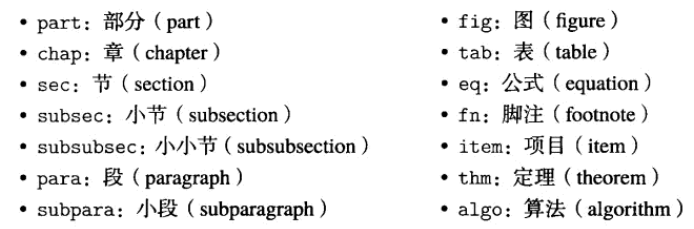
\includegraphics[width=\textwidth]{img//HowToName.png}
        \end{figure}
    \end{frame}
    
    \begin{frame}[fragile]
        \frametitle{pdf文件功能上的拓展}
        pdf文档支持很多特殊功能,如文档标签,超链接,电子表单等等,\LaTeX 也可以输出这样的功能,比如超链接,而这只需要添加一个宏包。
\begin{lstlisting}
% 在导言区(你最好不要忘了导言区是哪里)
% 插入下面的宏包
\usepackage{hyperref}
% 插入后,交叉引用会自动变为超链接。同样,至少编译两次
\end{lstlisting}
        \begin{itemize}
            \item 为刚才做的CrossReferences添加hyperref宏包,增加超链接
            \item 进入练习Hyperref中,猜测理解hypersetup中的内容。在pdf文件中,依次点击目录,公式标签,网页超链接,文件超链接,以及语句的链接。语句的链接可以注意一下,看看它是用了怎样的命令定位的。
        \end{itemize}
    \end{frame}



\subsection{索引}

    \begin{frame}[fragile]
    其实我觉得很多同学不知道什么叫索引。(快来打脸)
    \begin{figure}
    \centering
    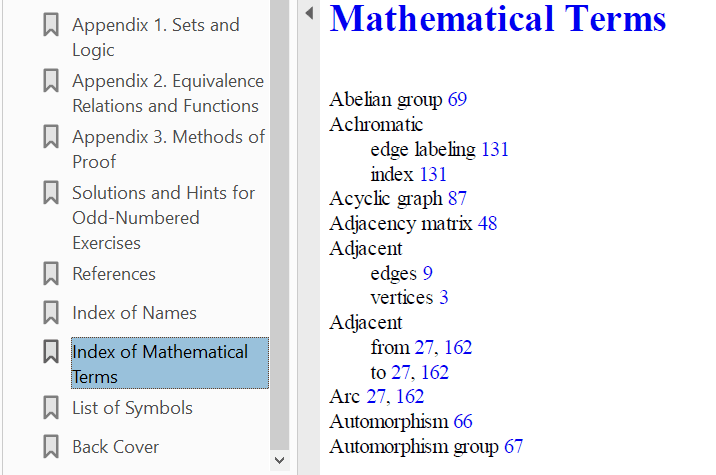
\includegraphics[width = 0.7\textwidth]{img//index.png}
    \end{figure}
    \end{frame}

    \begin{frame}[fragile]
    \frametitle{步骤}
    对tex文件,你需要做:
\begin{lstlisting}
导言区使用\makeindex
导言区调用makeidx宏包
需要索引的地方,使用\index{•}标记
在放索引的地方(通常是末尾),使用\printindex命令
\end{lstlisting}
    编译时,你需要:
\begin{lstlisting}
xelatex file_name
makeindex file_name
xelatex file_name
\end{lstlisting}
    注意:
    \begin{itemize}
        \item 配置好你的makeindex
        \item 不要忘了编译的次数和顺序
    \end{itemize}
    进入练习WordIndex,看看能不能编译出两个tex文件的索引
    \end{frame}

\subsection{文献引用}

    \begin{frame}[fragile]
        这块不细讲了,主要是编译的顺序
\begin{lstlisting}
xelatex filename
bibtex filename
xelatex filename
xelatex filename
\end{lstlisting}
         \begin{itemize}
             \item 在练习bib中按照上面的编译顺序,看看能否生成样例中的文件
             \item 在tex文件中用的指令,可去网上具体了解。
             \item 引用可以在tex文件中自己写,但用的比较多的是写在bib文件中(有专门的管理软件),最后导入,生成引用
         \end{itemize}
    \end{frame}




\section{其他}
    
    \begin{frame}[fragile]
        \frametitle{小建议}
        \begin{itemize}
            \item 要学会自学!自学!自学!
            \item 学会看错误日志(红色的那个),\textbf{耐下心来读英文}(其实不少人看到红色的字符串就不想认真读,然后自己肉眼挑BUG,或者问别人),自己解决不了的时候,一个很好的办法,是复制你的错误信息,以及你刚做的事的关键词(比如某个指令名),贴到搜索框搜索(当然是英文)\pause
             \item 对于上面这点,举个小例子:\verb|"!Undefined control sequence."|,这是一个伴随你一生的报错,绝大部分都可归为以下三种原因的一种:
                 \begin{itemize}
                     \item 拼错了!
                     \item 没导入宏包!
                     \item 用了不存在的指令!
                 \end{itemize}
        \end{itemize}
    \end{frame}
    
    \begin{frame}[fragile]{小建议}
        \begin{itemize}
            \item 另一位主讲人想要分享他昨晚(今天凌晨)的惨痛教训
            \item 遇到报错信息 \verb|Beamer - ! File ended while scanning use of \next|
            \item 尝试注释法肉眼找bug半小时无果
            \item 网上一查,错误原因是这样的
            \begin{figure}
                \centering
                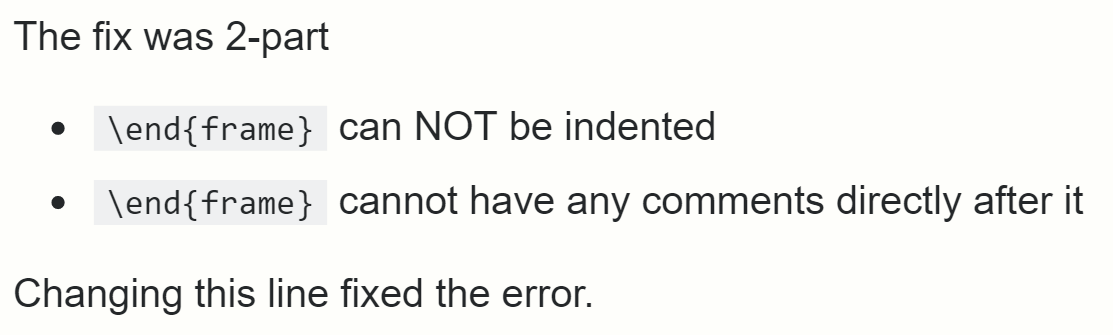
\includegraphics[width=.7\textwidth]{img/bug}
            \end{figure}
            \item 最后发现是在某个\verb|\end{frame}|后加了一个空格
        \end{itemize}
    \end{frame}
    
    \begin{frame}[fragile]
        \frametitle{小建议}
        \begin{itemize}
            \item 基础设施很重要!抽个时间,去专门学习你使用的编辑器是很有必要的。
            \item 关于上面这点,做些解释:
            \begin{itemize}
                \item 使用Tab键把你正在写的指令瞬间补全,也许就能省下百分之十的时间,积累起来就能让你多活一天!所以找个时间把常用的指令录进编辑器的代码补全里面是不是很有必要?(当然,花时间去网上找拓展包也是一样的)
                \item 再比如,自定义一个宏编译,设置为xelatex + bibtex + xelatex + xelatex,这样你按一个键就能完成引用的生成,是不是觉得很舒服?
                \item 夜晚看屏幕伤眼,心理也难受,所以换一个护眼又好看的主题皮肤是不是很好?
            \end{itemize}\pause
            \item 熟能生巧,可以渐渐用latex代替word去做平时的作业,可能一开始会有点慢,但当你渐渐熟悉自己的几个模板之后,速度就能反超word,还更好看
        \end{itemize}
    \end{frame}
    
    \begin{frame}[fragile]
        \begin{figure}
        
\includegraphics[width=0.45\textwidth]{img//tip.png}
        \end{figure}
        \begin{center}
        欢迎大家成为下一届学术软件教学系列讲座主讲人!
        \end{center}
    \end{frame}
    
    \begin{frame}[fragile]
        \frametitle{资源分享}
        \begin{itemize}
            \item \url{https://www.sharelatex.com/}
            \item \url{https://tex.stackexchange.com/}
            \item \url{http://tug.ctan.org/tex-archive/} 找文档,找手册!\\
            镜像站:\url{http://mirrors.ustc.edu.cn/CTAN/}
            \item \url{http://tug.org/}
        \end{itemize}
    \end{frame}
\end{document}
\end{lstlisting}
	\end{frame}

	\begin{frame}[fragile]
		\indent 划分文档的主要方式是\verb|\input{}|和\verb|\include{}|,将不同的章节内容写在不同的.tex文件中,用上述两种方式引入主文件中。\\
		\begin{description}
			\item[input] 相当于ctrl+c和ctrl+v,直接把代码复制过来,稳定、实用
			\item[include] 常和\verb|\includeonly|一起使用,可以选择性地编译子文件,常用于书籍之类的特大文档
		\end{description}
		\indent 两种方式的编译效果有细节上的不同,自己试试
	\end{frame}

	\begin{frame}
	截图来自stackexchange.com,题为input vs include
	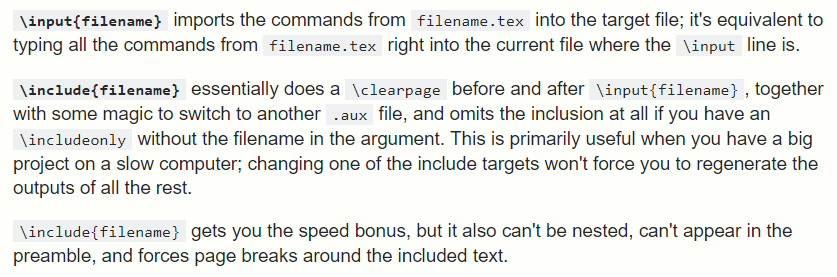
\includegraphics[width=\textwidth]{img//vs.png}	
	\end{frame}

	\begin{frame}[fragile]
		我们用的比较多的是input,当你觉得某一部分代码太长时,可以考虑写在别的.tex文件中,精简主文件,平时主要用在下面几种情况
		\begin{itemize}
			\item 导言区繁多的设置(通常会写在名为preamble的文件中,请看问求的作业模板)
			\item 异常庞大的表格
			\item 设置复杂的图片(比如需要使用很多子图subfig时)
		\end{itemize}
		此外可以去了解一下\verb|\endinput|的使用
	\end{frame}

\section{文本环境举隅}

\subsection{常用文本环境}

    \begin{frame}
    (其实会下面的就够了……)
    \begin{itemize}
        \item 文本环境:quote, quotation, abstarct(写诗的同学可以去了解verse)
        \item 列表环境:itemize, enumerate
        \item 定理类环境:thm, lemma, definition, proof
        \item 抄录和代码环境:verb, lstlisting
        \item 脚注:footnote
    \end{itemize}
    \end{frame}
    
    \begin{frame}
    \frametitle{练习和小建议}
    \begin{itemize}
    \item 打开练习list, theorem, listing$\_$code, page
    \item 想要用好文本环境,更建议看手册而不是上网搜索
    \end{itemize}
    \end{frame}
\section{中文支持}
\subsection{了解\CTeX}
\begin{frame}{How to get Chinese document?}{\CTeX}
	\CTeX 是最新的也是最便利的\LaTeX 中文支持的开源项目,可以参考其\href{material/LM/CTEXmanual.pdf}{\textcolor{blue}{使用手册}}。
	\begin{itemize}
		\item 全面汉化
		\item 更智能的排版
		\item 强大的自定义设置
	\end{itemize}
	一般使用默认设置即可,有特殊需求可翻阅手册作适当调整。
\end{frame}
\begin{frame}
	\begin{table}\caption{\CTeX 宏集的组成}
		\footnotesize
		\begin{tabular}{llp{6cm}}
			\toprule
			类别 & 文件 & 说明 \\
			\midrule
			文档类 & ctexart.cls & 标准文档类article 的汉化版本,一般适用于短篇幅的文章\\
			& ctexrep.cls & 标准文档类report 的汉化版本,一般适用于中篇幅的报告\\
			& ctexbook.cls & 标准文档类book 的汉化版本,一般适用于长篇幅的书籍\\
			& ctexbeamer.cls & 文档类beamer 的汉化版本,适用于幻灯片演示\\
			\midrule
			宏包 & ctex.sty & 提供全部功能,但默认不开启章节标题设置功能,需要使用heading 选项来开启\\
			& ctexsize.sty & 定义和调整中文字号,在ctex 宏包或CTEX 中文文档类之外单独调用\\
			& ctexheading.sty & 提供章节标题设置功能,在ctex 宏包或CTEX 中文文档类之外单独调用\\
			\bottomrule
		\end{tabular}
	\end{table}
\end{frame}
\begin{frame}[fragile]
	\begin{itemize}
		\item 文档类
\begin{lstlisting}
\documentclass{ctexart}
\documentclass{ctexrep}
\documentclass{ctexbook}
\documentclass{ctexbeamer}
\end{lstlisting}		
		\item 宏包
\begin{lstlisting}
\usepackage{ctex}
\usepackage{ctexsize}      
\usepackage{ctexheading}   
\end{lstlisting}
	\end{itemize}
	\vspace{2ex}
	\textcolor{red}{注意}:\texttt{ctexcap} 是默认打开 \texttt{heading} 选项的 \texttt{ctex} 宏包,手册中明确说明其为过时宏包!
\end{frame}
\begin{frame}
	两个最常用选项\texttt{heading}与\texttt{scheme}。

	打开\texttt{ctex.tex},体会不同选项的区别。
	\begin{itemize}
		\item \texttt{ctexart}类文档与\texttt{ctex}宏包的默认选项都是\texttt{heading=true,scheme=chinese}
		\item \texttt{heading=false,scheme=plain}相当于只是支持中文,所有的版式都还是英文的
		\item 如果觉得标题居中太蠢了想要靠左,可以用\texttt{heading=false}(\texttt{scheme=chinese}是默认选项不用改)
	\end{itemize}
\end{frame}
\section{强大的数学公式}
\begin{frame}[fragile]{写在前面}
	除了一些最简单的数学公式,大部分都需要宏包支持。建议平时需要输入公式时就直接使用以下四个宏包
\begin{lstlisting}
\usepackage{amsmath,amsfonts,amssymb,mathtools}
\end{lstlisting}
	这能够支持大多数的数学公式,而不必去纠结什么时候应该用哪一个、哪一个是多余的。

	\vspace{2ex}
	在讨论更多的数学环境前,我们统一使用 \cprotect\fbox{\verb|$|$\dots$\verb|$|} 输入行内(inline)公式,\cprotect\fbox{\verb|\[|$\dots$\verb|\]|} 输入行间(displayed)公式。

	\vspace{2ex}
	\textcolor{red}{注意}:凡是要用到数学字符的地方必须进入数学环境,有些字符虽然不在数学环境下也能输入,但是区别很大!
	\begin{table}
		\begin{tabular}{rlrl}
			\textrm{1+1=2} & $1+1=2$ \quad & \quad \textrm{a sin x} & $a \sin x$
		\end{tabular}
	\end{table}
\end{frame}

\subsection{数学符号}
\begin{frame}[fragile]{字母表与数学字体}
	在公式环境内默认使用 \cprotect\fbox{\verb|\mathnormal|} 字体,与正文环境下默认字体对比如下
	\begin{itemize}
		\item Capital
		\begin{itemize}
			\item \textrm{ABCDEFGHIJKLMNOPQRSTUVWXYZ}
			\item $ABCDEFGHIJKLMNOPQRSTUVWXYZ$
		\end{itemize}
		\item Lower case
		\begin{itemize}
			\item \textrm{abcdefghijklmnopqrstuvwxyz}
			\item $abcdefghijklmnopqrstuvwxyz$
		\end{itemize}
	\end{itemize}
	其明显特征是斜体且间距较正文大一些。

	\vspace{2ex}
	而\cprotect\fbox{\verb|\mathit|}, \cprotect\fbox{\verb|\mathrm|}, \cprotect\fbox{\verb|\mathbf|}, \cprotect\fbox{\verb|\mathsf|}, \cprotect\fbox{\verb|\mathtt|} 这些数学字体通常直接使用相对应的正文字体\cprotect\fbox{\verb|\text**|}。
\end{frame}
\begin{frame}[fragile]{选用正确的字体}
	\begin{itemize}
		\item 变量使用默认字体,如$x, y, z$
		\item $\mathrm{e}, \mathrm{i}$等常量应使用罗马体 \cprotect\fbox{\verb|\mathrm|}
		\item 集合$\mathbb{N}, \mathbb{R}$等可使用 \verb|amssymb|提供的黑板粗体 \cprotect\fbox{\verb|\mathbb|}
		\item 向量$\bm{v}$应加粗,实现方法有很多,这里推荐 \verb|bm| 宏包的 \cprotect\fbox{\verb|\bm|} 命令
	\end{itemize}
\end{frame}
\begin{frame}[fragile]{希腊字母}
	\begin{itemize}
		\item 小写希腊字母
		\begin{itemize}
			\item 一般 \cprotect\fbox{\verb|\+小写拼写|},如 \cprotect\fbox{\verb|\alpha|} 即输出$\alpha$
			\item 注意$\mu, \nu$分别为 \cprotect\fbox{\verb|\mu|},\cprotect\fbox{\verb|\nu|}
			\item 一部分希腊字母有变体,这些变体在数学公式中常常用到,只需在前面加上 \verb|var|
				\begin{itemize}
				\item[] \small $\epsilon \rightarrow \varepsilon$ \qquad $\phi \rightarrow \varphi$ \qquad
					$\theta \rightarrow \vartheta$ \qquad $\sigma \rightarrow \varsigma$ \qquad
					$\pi \rightarrow \varpi$
				\end{itemize}
		\end{itemize}
		\item 大写希腊字母
		\begin{itemize}
			\item 一部分大写希腊字母与拉丁字母形状相同,直接使用即可,如$\mathrm{A, B}$
			\item 将小写希腊字母输入时首字母大写即可得到其大写形式,如 \cprotect\fbox{\verb|\Gamma|} 得到$\Gamma$
			\item 大写希腊字母一般用正体,前面加 \cprotect\fbox{\verb|var|} 或使用 \cprotect\fbox{\verb|\mathnormal|} 可得到倾斜形式
		\end{itemize}
		\item 小写希腊字母直立体形式?
		\begin{itemize}
			\item 数字字体宏包 \verb|upgreek|,在前面加上 \cprotect\fbox{\verb|up|}
			\item \cprotect\fbox{\verb|\pi|} $\rightarrow$ \cprotect\fbox{\verb|\uppi|} \qquad $\pi \rightarrow \uppi$
		\end{itemize}
	\end{itemize}
\end{frame}
\begin{frame}[fragile]{常用符号}
	\begin{table}\caption{数学普通符号(部分)}
		\begin{tabular}{llllll}
			\toprule
			$\hbar$ & \verb|\hbar| & $\ell$ & \verb|\ell| & $\partial$ & \verb|\partial| \\
			$\infty$ & \verb|\infty| & $\prime$ & \verb|\prime| & $\emptyset$ & \verb|\emptyset| \\
			$\nabla$ & \verb|\nabla| & $\forall$ & \verb|\forall| & $\exists$ & \verb|exists| \\
			$\neg$ & \verb|\neg| & $\varnothing$ & \verb|\varnothing| & $\angle$ & \verb|\angle| \\
			$\clubsuit$ & \verb|\clubsuit| & $\diamondsuit$ & \verb|\diamondsuit| & $\heartsuit$ & \verb|\heartsuit| \\
			$\spadesuit$ & \verb|\spadesuit| & $\triangle$ & \verb|\triangle| & $\square$ & \verb|\square| \\
			$\flat$ & \verb|\flat| & $\natural$ & \verb|\natural| & $\sharp$ & \verb|\sharp|\\
			\bottomrule
		\end{tabular}
	\end{table}
\end{frame}
\begin{frame}[fragile]{常用符号}
	\begin{table}\caption{可同时用在文本和数学模式中的符号}
		\begin{tabular}{llllllll}
			\toprule
			$\#$ & \verb|\#| & $\&$ & \verb|\&| & $\%$ & \verb|\%| & $\$$ & \verb|\$| \\
			$\_$ & \verb|\_| & $\{$ & \verb|\{| & $\}$ & \verb|\}| & & \\
			$\P$ & \verb|\P| & $\S$ & \verb|\S| & $\dag$ & \verb|\dag| & $\ddag$ & \verb|\ddag| \\
			$\copyright$ & \verb|\copyright| & $\pounds$ & \verb|\pounds| & $\ldots$ & \verb|\ldots| & & \\
			$\checkmark$ & \verb|\checkmark| & $\circledR$ & \verb|\circledR| & $\maltese$ & \verb|\maltese| & $\yen$ & \verb|\yen| \\
			\bottomrule
		\end{tabular}
	\end{table}
	\begin{table}\caption{希伯来字母}
		\begin{tabular}{llllllll}
			\toprule
			$\aleph$ & \verb|\aleph| & $\beth$ & \verb|\beth| & $\daleth$ & \verb|\daleth| & $\gimel$ & \verb|\gimel| \\
			\bottomrule
		\end{tabular}
	\end{table}
\end{frame}
\begin{frame}[fragile]{数学算子}{Math operator}
	\begin{itemize}
		\item 巨算符(large operator)
		\begin{itemize}
			\item 所谓巨算符是大小可变的运算符
			\item 其在行内与行间大小是不同的
			\item 一般可以添加有上下标(数学结构中会讲)
			\item 行内行间上下标的形式也有所不同
		\end{itemize}
	\end{itemize}
	\begin{align*}
		\int_a^b & \textstyle \int_a^b & \iint_m^n & \textstyle \iint_m^n & \oint_{|z|=1} & \textstyle \oint_{|z|=1} \\
		\sum_{n=0}^{\infty} & \textstyle \sum_{n=0}^{\infty} & \prod_{1 \le i < j \le n} & \textstyle \prod_{1 \le i < j \le n} & \bigcup\nolimits_{i=1}^{n} & \textstyle \bigcup\limits_{i=1}^{n}
	\end{align*}
	\small \quad \cprotect\fbox{\verb|\limits|} \quad \cprotect\fbox{\verb|\nolimits|} \quad 行内公式尽量避免上下限放在算符上下位置
\end{frame}
\begin{frame}[fragile]{数学算子}{Math operator}
	\begin{itemize}
		\item 文字名称的算子
		\begin{itemize}
			\item 使用直立罗马体排印,一般 \cprotect\fbox{\verb|\+名称|} 即可
			\item 分为两类,带上下限的与不带上下限的
			\begin{itemize}
				\item $\log \quad \sin \quad \cosh \quad \arctan \quad \exp$ 
				\item $\lim \quad \max \quad \min \quad \sup \quad \inf$ 
			\end{itemize}
			\item 带上下限的算子使用起来与巨算符相似\\
				\qquad $\lim\limits_{x \to 0} \qquad \lim_{x \to 0}$
			\item 如果需要定义新的算子,可以在导言区使用 \verb|\DeclareMathOperator(*)|,带 \verb|*|表示带上下限
			\begin{itemize}
				\item \verb|\DeclareMathOperator{\arccot}{arccot}| \\ $\arccot$
				\item \verb|\DeclareMathOperator{\sign}{sgn}| \\ $\sign$
				\item \verb|\DeclareMathOperator*{\limsup}{lim\,sup}| \\ $\limsup$
			\end{itemize}
		\end{itemize}
	\end{itemize}
\end{frame}
\begin{frame}[fragile]{二元运算符与关系符}
	\begin{itemize}
		\item $\cprotect\overset{\cprotect\fbox{\scriptsize\verb|+|}}{+}, 
	\cprotect\underset{\cprotect\fbox{\scriptsize\verb|-|}}{-}, 
	\cprotect\overset{\cprotect\fbox{\scriptsize\verb|\times|}}{\times}, 
	\cprotect\underset{\cprotect\fbox{\scriptsize\verb|\div|}}{\div}$等二元运算符与
	$\cprotect\overset{\cprotect\fbox{\scriptsize\verb|=|}}{=}, 
	\cprotect\underset{\cprotect\fbox{\scriptsize\verb|>|}}{>}, 
	\cprotect\overset{\cprotect\fbox{\scriptsize\verb|<|}}{<}, 
	\cprotect\underset{\cprotect\fbox{\scriptsize\verb|\ne|}}{\ne}, 
	\cprotect\overset{\cprotect\fbox{\scriptsize\verb|\le|}}{\le}$\textrm{,} $
	\cprotect\underset{\cprotect\fbox{\scriptsize\verb|\ge|}}{\ge}$\textrm{,} $
	\cprotect\overset{\cprotect\fbox{\scriptsize\verb|\ll|}}{\ll}$\textrm{,} $
	\cprotect\underset{\cprotect\fbox{\scriptsize\verb|\gg|}}{\gg}$等关系符与前后变量之间会保留一定的空隙,且行内公式可以在它们的后面断行。
	\item 二元关系符数量庞大,除了一些最常用的,一般有需要的时候随用随查即可。
	\item 使用 \cprotect\fbox{\verb|\mathbin|} 和 \cprotect\fbox{\verb|\mathrel|} 可以将其参数当作二元运算符和二元关系符来对待,可用于定义新运算或一些其他用途。
	\item 箭头符号与逻辑符号使用时同样可以查阅,不再赘述。
	\end{itemize}
\end{frame}
\begin{frame}[fragile]{定界符}
	\[\{\frac{\partial y_j}{\partial x_i} | i=1,2,\cdots,n,\, j=1,2,\cdots,m\}\]
	\[\left\{\frac{\partial y_j}{\partial x_i} \middle| i=1,2,\cdots,n,\, j=1,2,\cdots,m\right\}\]
	上例中的$\{\,|\,\}$均为定界符,其大小可以根据式子的大小而改变。
	\begin{itemize}
		\item 括号定界符
		\[(\,)\quad[\,]\quad\{\,\}\quad\langle\,\rangle\quad\lfloor\,\rfloor\quad\lceil\,\rceil\]
		\item 非括号定界符
		\[/\quad\backslash\quad|\quad\|\]
		\item 输入
		\begin{itemize}
			\item \verb|( ) [ ] \{ \} \langle \rangle|\\
				\verb|\lfloor \rfloor \lceil \rceil|
			\item \verb!/ \backslash | \|!
		\end{itemize}
	\end{itemize}
\end{frame}
\begin{frame}[fragile]{如何确定定界符大小}
	\begin{itemize}
		\item 自动调整
		\begin{itemize}
			\item 使用 \cprotect\fbox{\verb|\left( ... \right)|},左右必须成对出现
			\item 如果只需要一个定界符,可以用 \cprotect\fbox{\verb|.|} 表示空的定界符,如 \cprotect\fbox{\verb|\left.|}
			\item 需要三个定界符的话可使用 \cprotect\fbox{\verb|\middle|} 放在中间,如前例
		\end{itemize}
		\item 手动调整
		\begin{itemize}
			\item 提供了 \cprotect\fbox{\verb|\big|},\cprotect\fbox{\verb|\Big|}, \cprotect\fbox{\verb|\bigg|},\cprotect\fbox{\verb|\Bigg|} 四种大小供手动调节
			\item 可以在后面加上 \cprotect\fbox{\verb|l m r|} 配套使用
			\item 自动调整效果不理想时,可以试试手动调整
			\item 在明确“左右”(如 \cprotect\fbox{\verb|\left \right|} 或 \cprotect\fbox{\verb|\Bigl \Bigr|})时,可直接使用 \cprotect\fbox{\verb|<>|} 表示尖括号而不致与$<>$混淆
		\end{itemize}
	\end{itemize}
\end{frame}
\begin{frame}[fragile]{标点符号}
	\begin{itemize}
		\item 数学环境内应使用英文标点,否则会报错
		\item 常用的标点符号有$, \quad ; \quad ! \quad ? \quad \colon$
		\item 应注意的是\cprotect\fbox{\verb|:|}是作为二元关系符存在的(如$f(x):=x, \{x : x>0\}$),而作为标点的冒号是 \cprotect\fbox{\verb|\colon|},其两侧间距不同,表示比例时则最好用 \cprotect\fbox{\verb|\mathbin{:}|}
		\item 省略号有很多种,在矩阵中常用到,平时最常用的是 \cprotect\fbox{\verb|\cdots|} $\cdots$ 和 \cprotect\fbox{\verb|\ldots|} $\ldots$ (或直接使用 \cprotect\fbox{\verb|\dots|} 让latex自己选择)
		\item 标点后是无法换行的,像$f(x,y,z)$谁也不希望在中间断行,而$a_1$\textrm{,} $a_2$\textrm{,} $a_3$\textrm{,} $\cdots$\textrm{,} $a_n$希望能断行时应将标点置于数学环境之外并加上空格
		\item 数学环境中空格不起作用,但可以分隔各部分让公式结构更清晰
	\end{itemize}
\end{frame}

\subsection{数学结构}
\begin{frame}[fragile]{上下标}
	\begin{itemize}
		\item 上标用 \verb|^| 表示,下标用 \verb|_| 表示
		\item 超过一个字符时就应使用$\{\,\}$
		\item \verb|'| 是一种特殊的上标,相当于 \cprotect\fbox{\verb|^\prime|}
		\item 使用 \cprotect\fbox{\verb|\overset|} 和 \cprotect\fbox{\verb|\underset|}可以在任意符号上下方添加标记
	\end{itemize}
\end{frame}
\begin{frame}[fragile]{分式}
	\begin{itemize}
		\item 使用 \cprotect\fbox{\verb|\frac{num}{den}|} 输入分式,先输入分子(numerator),后输入分母(denominator)
		\item 行内默认使用正文格式(text style)分式,行间默认使用显示格式(display style)分式,可以使用 \cprotect\fbox{\verb|\tfrac|} 与 \cprotect\fbox{\verb|\dfrac|} 指定使用某一种
		\item 行内使用分式时,$a/b$效果往往比$\frac ab$更好
		\item 连分式用 \cprotect\fbox{\verb|\cfrac|},这里不细讲
		\item 顺带一提,\cprotect\fbox{\verb|\textstyle|} 和 \cprotect\fbox{\verb|\displaystyle|} 可以指定整条公式以哪种方式显示
	\end{itemize}
\end{frame}
\begin{frame}[fragile]{根式}
	\begin{itemize}
		\item \cprotect\fbox{\verb|\sqrt[root]{arg}|}
		\item \texttt{[\,]}内为可选项,用\cprotect\fbox{\verb|\uproot|} 与 \cprotect\fbox{\verb|\leftroot|} 可以微调\texttt{root}位置,参数为整数
		\item 被开方数不是整数或结构复杂时,通常改用等价的指数形式
		\item 使用 \cprotect\fbox{\verb|\vphantom|} 占位来获得统一的高度\\[1ex]
		\verb|\sqrt{\frac 12} < \sqrt{\vphantom{\frac12}2}|
		\[\sqrt{\frac 12} < \sqrt{\vphantom{\frac12}2}\]
		\item \cprotect\fbox{\verb|\mathstrut|} 用来平衡不同高度和深度的字母\\[1ex]
		\verb|\sqrt b \sqrt y|\\
		\verb|\sqrt{\mathstrut b} \sqrt{\mathstrut y}|
		\[\sqrt b \sqrt y \quad \rightarrow \quad \sqrt{\mathstrut b} \sqrt{\mathstrut y}\]
	\end{itemize}
\end{frame}
\begin{frame}[fragile]{矩阵}
	\begin{itemize}
		\item 输入矩阵结构需要矩阵环境,它们的区别在于外面的括号不同
		\begin{itemize}
			\item \texttt{ matrix}环境 \quad 无括号
			\item \texttt{pmatrix}环境 \quad 圆括号
			\item \texttt{bmatrix}环境 \quad 方括号
			\item \texttt{Bmatrix}环境 \quad 大括号
			\item \texttt{vmatrix}环境 \quad 单竖线
			\item \texttt{Vmatrix}环境 \quad 双数线
		\end{itemize}
		\item 以一个最简单的二阶矩阵为例\\
		\begin{minipage}[c]{0.5\textwidth}
\begin{lstlisting}
\[ \begin{pmatrix}
       a_{11} & a_{12} \\
       a_{21} & a_{22}
   \end{pmatrix} \]
\end{lstlisting}
		\end{minipage}
		\begin{minipage}[c]{0.4\textwidth}
			\[ \begin{pmatrix}
				a_{11} & a_{12} \\
				a_{21} & a_{22}
			\end{pmatrix} \]
		\end{minipage}
	\end{itemize}
\end{frame}
\subsection{数学环境}
\begin{frame}[fragile]{概述}
	我们先前使用的 \cprotect\fbox{\verb|\[|$\dots$\verb|\]|} 实质是
\begin{lstlisting}
\begin{equation*}
    ...
\end{equation*}
\end{lstlisting}
	的缩写,其中“$*$”表示不给该公式标序。

	\vspace{2ex}
	出于各方面的需求,我们并不满足于这样一个简单居中、无法换行的数学环境,而是会有诸多其他方面的要求。这时我们需要更多的数学环境来提供支持。
\end{frame}
\begin{frame}[fragile]{多行公式}{每行均为一个公式}
	\begin{itemize}
		\item 简单的多个公式罗列: \verb|gather(*)|
		\begin{itemize}
			\item 每行公式都是居中显示的
			\item 使用 \cprotect\fbox{\verb|\\|} 换行
			\item 某行不需要编号,在 \cprotect\fbox{\verb|\\|} 前加  \cprotect\fbox{\verb|\notag|} 
		\end{itemize}
		\item 公式按关系符对齐: \verb|align(*)|
		\begin{itemize}
			\item 使用 \cprotect\fbox{\verb|\\|} 换行,关系符前加 \cprotect\fbox{\verb|&|} 表示对齐
			\item \cprotect\fbox{\verb|&|} 一般放在二元关系符($=,<,>$等)前面
			\item 有时可巧用 \cprotect\fbox{\verb|\phantom|} 变通 
		\end{itemize}
		\item 多行公式每行都会产生一个编号,不希望产生的话可以使用\cprotect\fbox{\verb|\notag|}
	\end{itemize}
\end{frame}
\begin{frame}
	练习:尝试输出以下公式。

	\begin{minipage}{0.95\textwidth}
	\begin{gather}
		\partialratio{A}{x}{y} = \lim_{\Delta x \to 0} \frac{f(x+\varDelta x,y)-f(x,y)}{\varDelta x} \\
		\partialratio{A}{y}{x} = \lim_{\Delta y \to 0} \frac{f(x,y+\varDelta y)-f(x,y)}{\varDelta y}
	\end{gather}
	\hrule
	\begin{align}
		& \mathrel{\phantom{=}} (a + b)(a^2 - ab + b^2)\notag \\
		& = a^3 - a^2b + ab^2 + a^2b - ab^2 + b^3\notag \\
		& = a^3 + b^3
	\end{align}
	\end{minipage}
\end{frame}
\begin{frame}[fragile]{多行公式}
	\begin{itemize}
		\item \verb|align(*)| 的另一个用处:排版多列公式
		\begin{itemize}
			\item 每行的基本格式
			\begin{itemize}
				\item[] \verb|a &= b  &  c &= d  &  e &= f \\|
			\end{itemize}
			\item 最后一行不需要 \cprotect\fbox{\verb|\\|}
			\item 按照行来标序
			\item \cprotect\fbox{\verb|&|} 必然为奇数个,出现偶数个会报错(为什么?)
		\end{itemize}
		\item 关于 \verb|flalign(*)|
		\begin{itemize}
			\item 与 \verb|align(*)| 是类似的
			\item 会把多列公式水平方向分散对齐
		\end{itemize}
		\item 关于 \verb|alignat(*)|
		\begin{itemize}
			\item 与 \verb|align(*)| 也是类似的
			\item 不会主动产生间距,需要手动输入间距大小
			\item 需要一个参数表示每行要对齐的公式个数
		\end{itemize}
	\end{itemize}
\end{frame}
\begin{frame}[fragile]
	对比 \verb|align(*)| 与 \verb|flalign(*)|

	\vspace{2ex}
	\clean
	\begin{minipage}{0.49\textwidth}
		\begin{itemize}
			\item 使用 \verb|align|
			\begin{align}
				x + y &= 2 & x &= 1 \\
				x - y &= 0 & y &= 1
			\end{align}
		\end{itemize}
	\end{minipage}
	\clean
	\begin{minipage}{0.49\textwidth}
		\begin{itemize}
			\item 使用 \verb|flalign|
			\begin{flalign}
				x + y &= 2 & x &= 1 \\
				x - y &= 0 & y &= 1
			\end{flalign}
		\end{itemize}
	\end{minipage}

	\vspace{3ex}
	巧用 \verb|alignat|(使用 \verb|align|必须借助 \cprotect\fbox{\verb|\phantom|})

	\begin{minipage}{0.69\textwidth}
\begin{lstlisting}
\begin{alignat*}{5}
    &1 & &+2 & &+3 & &+4 & &=10 \\
    &1 & &   & &+3 & &   & &=4 \\
    &  & &+2 & &   & &+4 & &=6
\end{alignat*}
\end{lstlisting}			
	\end{minipage}
	\begin{minipage}{0.29\textwidth}
		\begin{alignat*}{5}
			&1 & &+2 & &+3 & &+4 & &=10 \\
			&1 & &   & &+3 & &   & &=4 \\
			&  & &+2 & &   & &+4 & &=6
		\end{alignat*}
	\end{minipage}
\end{frame}
\begin{frame}[fragile]{多行公式}
	\begin{itemize}
		\item 如何在多行公式之间插入说明性文字?
		\begin{itemize}
			\item 每次都退出数学环境输入文字过于麻烦
			\item 退出数学环境会破环上下公式间对齐关系
		\end{itemize}
		\item \cprotect\fbox{\verb|\text|} 行内插入文字
		\item \cprotect\fbox{\verb|\intertext|} 换行顶格插入文字(前一行的 \cprotect\fbox{\verb|\\|} 可省略)
		\item \cprotect\fbox{\verb|\shortintertext|} 提供更为紧凑的行间距
	\end{itemize}
\end{frame}
\begin{frame}
	例:

	\vspace{2ex} \clean
	绝热过程中,$Q=0$,不做非膨胀功时,有
	\begin{gather}
		\di U = \delta W
		\quad \text{或} \quad
		\di U + p \di V = 0
		\shortintertext{已知}
		\todi{U}{T}{V}
		\shortintertext{对理想气体,}
		\di U = C_V \di T, \quad \Delta U = \int_{T_1}^{T_2}C_V \di T
		\intertext{若$C_V$为常数,}
		\Delta U = C_V(T_2-T_1) = W
	\end{gather}
\end{frame}
\begin{frame}[fragile]{多行公式}
	\begin{itemize}
		\item 多个联系紧密的公式如何共用一个编号?
		\begin{itemize}
			\item[] 使用 \verb|subequations| 环境
		\end{itemize}
		\item 示例:
\begin{lstlisting}
\begin{subequations}
\begin{align}
  a \cdot b &= b \cdot a \\
  (a \cdot b) \cdot c &= a \cdot (b \cdot c) \\
  a \cdot (b + c) &= a \cdot b + a \cdot c 
\end{align}
\end{subequations}
\end{lstlisting}
		\clean \vspace{-0.5cm}
		\begin{minipage}{0.7\textwidth}
			\begin{subequations}
				\begin{align}
					a \cdot b &= b \cdot a \\
					(a \cdot b) \cdot c &= a \cdot (b \cdot c) \\
					a \cdot (b + c) &= a \cdot b + a \cdot c 
				\end{align}
			\end{subequations}
		\end{minipage}
	\end{itemize}
\end{frame}
\begin{frame}
练习:尝试输出如下的麦克斯韦方程组。

	\vspace{2ex} \clean
\begin{minipage}[t]{0.54\textwidth}
	\begin{itemize}
		\item 积分形式
	\end{itemize}
\end{minipage}
\quad
\begin{minipage}[t]{0.4\textwidth}
	\begin{itemize}
		\item 微分形式
	\end{itemize}
\end{minipage}
\begin{minipage}[c]{0.54\textwidth}
	\begin{subequations}
		\begin{align}
			\varoiint_S \bm{D} \cdot \di \bm{S} &= q, \\
			\varoiint_S \bm{B} \cdot \di \bm{S} &= 0, \\
			\oint_L \bm{E} \cdot \di \bm{\ell} &= - \iint \frac{\partial \bm{B}}{\partial\, t} \cdot \di \bm{S}, \\
			\oint_L \bm{H} \cdot \di \bm{\ell} &= I_0 + \iint \frac{\partial \bm{D}}{\partial\, t} \cdot \di \bm{S}.
		\end{align}
	\end{subequations}
\end{minipage}
\quad
\begin{minipage}[c]{0.4\textwidth}
	\begin{subequations}
		\begin{align}
			\nabla \cdot \bm{D} &= \rho_f, \\
			\nabla \cdot \bm{B} &= 0, \\
			\nabla \times \bm{E} &= -\frac{\partial \bm{B}}{\partial\, t}, \\
			\nabla \times \bm{H} &= \bm{J}_f + \frac{\partial \bm{D}}{\partial\, t}.
		\end{align}
		\end{subequations}		
	\end{minipage}
\end{frame}
\begin{frame}{拆分公式}{整体为一个公式}
	行内公式中,对于长公式如$1+2+3+4+5+6+7+8+9+10+11+12+13+14+15+16+17+18+19+20+21+22+23+24+25+26+27+28+29+30$我们先前提过是可以在二元运算符后换行的,但是对于行间公式则不然,见下例。
	\[
	1+2+3+4+5+6+7+8+9+10+11+12+13+14+15+16+17+18+19+20+21+22+23+24+25+26+27+28+29+30
	\]
	这时候可以使用\texttt{multline(*)}环境。(注意不是 \textcolor{red}{\texttt{multiline}}!)
\end{frame}
\begin{frame}[fragile]
\begin{lstlisting}
\begin{multline}
    1+2+3+4+5+6+7 \\
    +8+9+10+11+12+13 \\
    +14+15+16+17+18+19+20+21 \\
    +22+23+24+25 \\
    +26+27+28+29+30
\end{multline}
\end{lstlisting}
	\clean
	\begin{multline}
		1+2+3+4+5+6+7 \\
		+8+9+10+11+12+13 \\
		+14+15+16+17+18+19+20+21 \\
		+22+23+24+25 \\
		+26+27+28+29+30
	\end{multline}
\end{frame}
\begin{frame}[fragile]{拆分公式}
	\begin{itemize}
		\item 可以看出\texttt{multline}环境中首行是左对齐的,尾行是右对齐的,中间行则是居中
		\item 公式的左右边距是通过长度变量\cprotect\fbox{\verb|\multlinegap|} 和 \cprotect\fbox{\verb|\multlinetaggap|} 设置的
		\item \cprotect\fbox{\verb|\shoveleft{}|} 和 \cprotect\fbox{\verb|\shoveright{}|} 可设置中间行像首尾两行那样左/右对齐
	\end{itemize}
	\setlength{\multlinegap}{4em}
	\setlength{\multlinetaggap}{4em}
	\begin{multline*}
		1+2+3+4+5+6+7 \\
		\shoveright{+8+9+10+11+12+13} \\
		+14+15+16+17+18+19+20+21 \\
		\shoveleft{+22+23+24+25} \\
		+26+27+28+29+30
	\end{multline*}
\end{frame}
\begin{frame}[fragile]
\begin{lstlisting}
\setlength{\multlinegap}{4em}
\setlength{\multlinetaggap}{4em}
\begin{multline*}
    1+2+3+4+5+6+7 \\
    \shoveright{+8+9+10+11+12+13} \\
    +14+15+16+17+18+19+20+21 \\
    \shoveleft{+22+23+24+25} \\
    +26+27+28+29+30
\end{multline*}
\end{lstlisting}
\end{frame}
\begin{frame}[fragile]{拆分公式}
	\begin{itemize}
		\item 如果想要在等号处对齐,可以考虑\texttt{split}环境
		\item \texttt{split}环境应当内嵌于\texttt{equation}中,使用方法上与\texttt{align}等类似
	\end{itemize}
	\clean
	\begin{minipage}{0.43\textwidth}
\begin{lstlisting}
\begin{equation}
\begin{split}
(AB)(B^{-1}A^{-1}) 
&= A(BB^{-1})A^{-1} \\
&= AIA^{-1} 
 = AA^{-1} \\
&= I
\end{split}
\end{equation}
\end{lstlisting}
	\end{minipage}
	\begin{minipage}{0.56\textwidth}
		\begin{equation} \begin{split}
			(AB) (B^{-1}A^{-1}) &= A(BB^{-1})A^{-1} \\
			&= AIA^{-1} = AA^{-1} \\
			&= I
		\end{split} \end{equation}
	\end{minipage}
\end{frame}
\begin{frame}[fragile]{组合成块}
	如何输入分段函数,如
	\[ \sign x = \begin{cases}
	1, & x > 0, \\
	0, & x = 0, \\
	-1, & x < 0.
	\end{cases} \]

	使用\texttt{cases} 环境(同样需要内嵌在\texttt{equation}等环境中)。
\begin{lstlisting}
\[ \sign x = \begin{cases}
  1, & x > 0, \\
  0, & x = 0, \\
  -1, & x < 0.
\end{cases} \]
\end{lstlisting}
\end{frame}

\begin{frame}{组合成块}
	\begin{itemize}
		\item 使用\texttt{dcases}环境得到显示格式大小的公式
		\item 此外使用上述部分环境的\texttt{+ed}模式能得到更多的将公式组合成块的应用
		\begin{itemize}
	 		\item 如:\texttt{gathered}, \texttt{aligned}, \texttt{alignedat}, \texttt{multilined}
	 		\item \texttt{lgathered}与\texttt{rgathered}可以设置环境内的若干行公式左对齐或右对齐,配合定界符使用
	 	\end{itemize}
	 	\item 以上环境的使用方法不变,它们都将多行的公式组合成块放在了一个公式环境内
	 	\item 这里只举几个例子,请自行融会贯通
	\end{itemize}
	\centering
	\texttt{请打开文件equation.tex并编译。}
\end{frame}
\section{图表与浮动体}

\subsection{构建表格}
\begin{frame}{tabular与array}
	\begin{itemize}
		\item tabular主要用于文本环境(数学模式下也可使用,但是还是按照文本模式排版)
		\item array用在数学环境中,主要用于排版复杂矩阵等包含数学符号的公式
		\item 二者用法上是相似的,这里只讲tabular
	\end{itemize}
\end{frame}
\begin{frame}[fragile]{基本格式}
\begin{lstlisting}
\begin{tabular}[<垂直对齐>]{<列格式说明>}
%   \hline
    <表项> & <表项> & ... & <表项> \\
%   \hline
    ...
\end{tabular}
\end{lstlisting}
	\begin{itemize}
		\item 垂直对齐选项可选填
		\begin{itemize}
			\item \texttt{t} \qquad 按表格顶部对齐
			\item \texttt{b} \qquad 按表格底部对齐
			\item \texttt{< >} \quad 垂直居中
		\end{itemize}
		\item 列格式说明符最基本的有
		\begin{itemize}
			\item \texttt{l} \quad 本列左对齐
			\item \texttt{c} \quad 本列居中
			\item \texttt{r} \quad 本列右对齐
			\item \texttt{|} \quad 列之间的竖线
		\end{itemize}
	\end{itemize}
\end{frame}
\begin{frame}[fragile]
	\begin{itemize}
		\item 每行单元格之间以 \verb|&|相隔,\verb|\\|用来换行
		\item 单元格内进行的设置作用域仅局限于本单元格
		\item \cprotect\fbox{\verb|\hline|} 表示两行间添加一条横线
	\end{itemize}
	例:

	这是一张表格:
	\begin{tabular}[b]{|c|lr|}
		\hline
		\bfseries 居中 & \ttfamily 靠左 & \rmfamily \itshape 靠右 \\
		\hline
		11111111 & 2222 & 4444444 \\
		abcdef & ghijklm & nopqrstuvwxyz \\
		\hline
	\end{tabular}
\begin{lstlisting}
这是一张表格:
\begin{tabular}[b]{|c|lr|}
\hline
\bfseries 居中 & \ttfamily 靠左 & \rmfamily\itshape 靠右 \\
\hline
11111111 & 2222 & 4444444 \\
abcdef & ghijklm & nopqrstuvwxyz \\
\hline
\end{tabular}
\end{lstlisting}
\end{frame}
\begin{frame}[fragile]
	\begin{itemize}
		\item 更多列格式说明符
		\begin{itemize}
			\item \verb|p{<宽>}| 本列具有固定宽度且可以自动换行,用于处理过多字符的单元格
			\item \verb|@{<内容>}} 将\texttt{<内容>}|作为两列之间的间隔,同时会取消列间的空隙
			\item \verb|*{<计数>}{<列格式说明>}| 将\verb|<列格式说明>|重复\verb|<计数>|次
		\end{itemize}
	\end{itemize}
	\begin{table}
		\centering
		\begin{tabular}{|c|*{3}{r@{.}l|}p{4em}|}
			\hline
			姓名 & \multicolumn{2}{c|}{收入} & \multicolumn{2}{c|}{支出} & \multicolumn{2}{c|}{结余} & \multicolumn{1}{c|}{备注} \\
			\hline
			qaq & 500 & 01 & 297 & 74 & 202 & 27 & 勤俭持家\\
			\hline
			orz & 50000 & 00 & 135345 & 53 & -85345 & 53 & 这太太太太太太有钱了 \\
			\hline
		\end{tabular}
	\end{table}
\end{frame}
\begin{frame}[fragile]
\begin{lstlisting}
\begin{tabular}{|c|*{3}{r@{.}l|}p{4em}|}
\hline
姓名 & \multicolumn{2}{c|}{收入} & \multicolumn{2}{c|}{支出} & \multicolumn{2}{c|}{结余} & \multicolumn{1}{c|}{备注} \\
\hline
qaq & 500 & 01 & 297 & 74 & 202 & 27 & 勤俭持家\\
\hline
orz & 50000 & 00 & 135345 & 53 & -85345 & 53 & 这太太太太太太有钱了 \\
\hline
\end{tabular}
\end{lstlisting}
\end{frame}
\begin{frame}[fragile]{单元格的合并与拆分}
	\begin{itemize}
		\item 使用 \cprotect\fbox{\verb|\multicolumn{cols}{pos}{text}|} 来合并列
		\begin{itemize}
			\item \texttt{cols} 选择需要合并的列数(大于等于1)
			\item \texttt{pos} 选择合并得的新单元格对齐方式
			\item \texttt{text} 输入单元格内容
		\end{itemize}
		\item 可以只合并1列,目的是暂时改变该列的对齐方式
		\item 合并行可以使用\texttt{multirow}宏包,与\verb|\cline{i=j}|配合使用
		\item 用\verb|\vline|制造竖线,达成拆分目的,但是间距不易掌握
		\item 可以在表格内嵌套表格来拆分,注意被嵌套的表格左右两边都应该是\texttt{@\{\}}
		\item \verb|\makecell|了解一下
		\item 骚操作有很多,但是我不会
		\item 有需要自己查
	\end{itemize}
\end{frame}
\begin{frame}[fragile]
	思考:
\begin{lstlisting}
\begin{tabular}{|p{8em}|p{8em}|p{8em}|}
\hline
默认靠左 & \centering 这里居中 & \multicolumn{1}{c|}{这里也居中} \\%最右边为什么不能用\centering?
\hline
\raggedleft 右对齐 & \multicolumn{1}{r|}{也右对齐惹} & 啦啦啦 \\%尝试只排版一排,你发现了什么?
\hline
\end{tabular}
\end{lstlisting}
	\begin{tabular}{|p{8em}|p{8em}|p{8em}|}
		\hline
		默认靠左 & \centering 这里居中 & \multicolumn{1}{c|}{这里也居中} \\
		\hline
		\raggedleft 右对齐 & \multicolumn{1}{r|}{也右对齐惹} & 啦啦啦 \\
		\hline
	\end{tabular} \\[1ex]
	\begin{tabular}{|p{8em}|p{8em}|p{8em}|}
		\hline
		默认靠左 & \centering 这里居中 & \multicolumn{1}{c|}{这里也居中} \\
		\hline
	\end{tabular} \\[1ex]
	\begin{tabular}{|p{8em}|p{8em}|p{8em}|}
		\hline
		\raggedleft 右对齐 & \multicolumn{1}{r|}{也右对齐惹} & 啦啦啦 \\
		\hline
	\end{tabular}
\end{frame}
\begin{frame}[fragile]{定宽表格与长表格}
	\begin{itemize}
		\item 定宽表格可以固定表格总宽度(如等于页宽)
		\item 可以使用\texttt{tabular*}环境,举个例子\\
\begin{lstlisting}
\begin{tabular*}{\textwidth}{|c@{\extracolsep{\fill}}ccccc|}
\end{lstlisting}
		\item 也可以用\texttt{tabularx}宏包提供的\texttt{tabularx}环境
		\item 长表格往往需要分页
		\item 可使用\texttt{longtable}宏包提供的\texttt{longtable}环境
	\end{itemize}
\end{frame}
\begin{frame}[fragile]{三线表}
	\begin{itemize}
		\item 在科技文档中大量使用三线表,三条表格线粗细不同,可以使用\texttt{booktabs}宏包。
		\item 大致结构如下
\begin{lstlisting}
%\usepackage{booktabs}
\begin{tabular}{ccccc}
  \toprule
% 表头
  \midrule
% 内容
  \bottomrule
\end{tabular} 
\end{lstlisting}
	\end{itemize}
\end{frame}

\subsection{插入图片}
\begin{frame}[fragile]{插入图片}
	\begin{itemize}
		\item 插入外部图片需要使用宏包\texttt{graphicx}
		\item 使用的命令与格式\\
\begin{lstlisting}
%\usepackage{graphicx}
\includegraphics[<选项>]{<文件名>}
\end{lstlisting}
		\item 文件名一般可以省略拓展名,默认与\texttt{tex}文档处于同一路径下 
	\end{itemize}
	\begin{center}
	\verb|\includegraphics{picname}|
	\end{center}
\end{frame}
\begin{frame}{拓展名}
	\begin{itemize}
		\item 最初\LaTeX 支持的图片格式有限,往往需要将图片转换格式后才能插入
		\item \XeLaTeX 支持的图片格式有\textrm{EPS, PDF, PNG, JPEG, BMP}等
		\item 除非遇到同一路径下两张图片名称相同拓展名不同,否则可以省略拓展名
	\end{itemize}
\end{frame}
\begin{frame}[fragile]{文件位置}
	\begin{itemize}
		\item 对于不是同一路径下的图片,可以使用其相对路径或绝对路径来插入图片
		\item 不论操作系统是什么,两层路径之间统一使用\texttt{/}来分隔
		\item 相对路径的可移植性比较高,也对于图片较多的情况也有利于文件的整理
		\begin{itemize}
			\item 如图片\texttt{selfie.jpg}位于当前路径下一个名为\texttt{pic}的文件夹内,可使用 \verb|\includegraphics{pic/selfie}|
			\item 如图片\texttt{logo.pdf}位于当前路径的上一层目录下,可使用 \verb|\includegraphics{../logo}|
		\end{itemize}
		\item 绝对路径不推荐使用,建议把图片复制到文档同一路径或相近路径下
		\begin{itemize}
			\item \verb|\includegraphics{C:/Users/username/Pictures/xx}|
			\item \verb|\includegraphics{home/username/Pictures/xx}|
		\end{itemize}
	\end{itemize}
\end{frame}
\begin{frame}[fragile]{可选选项}
	\begin{itemize}
		\item \texttt{[ ]}内可以选填的内容有很多,最常用的是设置其图片大小
		\item 默认的图片尺寸是其自然尺寸,对于矢量图是制作的尺寸,对于位图则是点阵数处以图形打印度(DPI)
		\item 最常用的设置大小的尺寸是\texttt{width},\texttt{height}和\texttt{scale}
		\item 举例
\begin{lstlisting}
\includegraphics[width=\textwidth]{pic1}
\includegraphics[height=4cm]{pic2}
\includegraphics[scale=.3]{pic3}
\end{lstlisting}
		\item 此外还有一些其他选项,查阅手册或阅读刘海洋的《LaTeX~入门》都可以学习
		\item 对图片还能做一些基本的变换
	\end{itemize}
\end{frame}

\subsection{绘图语言}
\begin{frame}{强大的内置绘图功能}
	\begin{itemize}
		\item 高端操作,超出本次讲座范围
		\item \xout{其实我也不会}
		\item \sout{大佬学会了教教我}
		\item \href{http://topspeedsnail.com/latex-circuitikz-circuit/}{\textcolor{blue}{这里}}有一个使用\texttt{circuitikz}绘制电路图的教程,更多的资料也可以从书籍或网站上找到
	\end{itemize}
\end{frame}

\subsection{浮动体与标题控制}
\begin{frame}
	\centering
	\Huge 公式和浮动体是\LaTeX 完爆Word的两个方面!!
\end{frame}
\begin{frame}[fragile]{浮动体环境}
	直接插入图片或表格的情况下是图(表)文混在一起的,但大多数情况下我们需要把图(表)插在段落之间或单独成页,并配以标题,同时对图片的确切位置没有精确的要求,只要插在某段话附近即可。这时就需要用到浮动体环境。
	\begin{itemize}
		\item 对于图片与表格分别有两类对应的浮动体环境:\texttt{figure}和\texttt{table}
		\item \texttt{figure}为例,基本语法格式为(\texttt{table}类似)
\begin{lstlisting}
\begin{figure}[<允许位置>]
    <任意内容>
\end{figure}
\end{lstlisting}
		\item \verb|<允许位置>|的可选项有\texttt{htbp}
		\begin{itemize}
			\item \quad \texttt{h} here \qquad \texttt{t} \quad top \qquad \texttt{b} \quad bottom \qquad \texttt{p} \quad page
		\end{itemize}
	\end{itemize}
\end{frame}
\begin{frame}[fragile]
	\begin{itemize}
		\item 允许位置的可选项可以只有一个,也可以是多个的组合,如 \verb|[htp]|则表示不允许\texttt{b}
		\item 不填则默认是 \verb|[htbp]|
		\item 顺序无关紧要,因为总是按照 \verb|[htbp]|的顺序来尝试
		\item 对于单独的\texttt{h},很多时候并不能得到令人满意的结果,因此latex会放宽为 \verb|[ht]|
		\item 若一定要用\texttt{h},可以采用 \verb|[!h]|
	\end{itemize}
\end{frame}
\begin{frame}{浮动体的本质}
	\begin{itemize}
		\item Q: 浮动体仅仅是用来插图表的吗?
		\item A: 不是的,浮动体里可以放入任意内容(一段文字,一段长代码,一组大型公式等)。
		\item Q: \texttt{figure}和\texttt{table}有什么区别,是不是前者只能用来插图片后者只能用来插表格?
		\item A: 不是的,前面已经说过插的东西是任意的。只是习惯上人们这么干,这与默认生成的标题有关。
		\item Q: 浮动体的本质是什么?
		\item A: 是一个可以活动的“盒子”。
		\item \sout{Q: 人类的本质是什么?}
		\item \sout{A: 人类的本质是什么?}
	\end{itemize}
\end{frame}
\begin{frame}[fragile]{caption与label}
	\begin{itemize}
		\item 使用\verb|\caption{<title>}|可以为浮动体加上标题,标题可换行
		\item 通常对于图片标题在下方,而对于表格标题在上方
		\item 默认情况下\texttt{figure}浮动体产生的标题将注明\texttt{Figure X},\texttt{table}浮动体产生的标题将注明\texttt{Table X},\texttt{X}是数字,由计数器控制
		\item 使用\texttt{ctex}的中文文档则相应地为\texttt{图 X}和\texttt{表 X}
		\item 这就是为什么通常\texttt{figure}用来插入图片而\texttt{table}用来插入表格,事实上这是可以更改的
		\item 在\texttt{caption}后加入\verb|\label{<lbl>}|,可用于交叉引用
	\end{itemize}
\end{frame}
\begin{frame}[fragile]{多栏下浮动体宽度}
	\begin{itemize}
		\item 使用命令\verb|\twocolumn|即可设置文档为双栏
		\item 多栏下\texttt{figure}和\texttt{table}浮动体只会占用一栏(宽度为\verb|\columnwidth|)
		\item 可以使用\texttt{figure*}和\texttt{table*}得到跨栏排版的浮动体
		\item 跨栏排版只允许\texttt{tp}两个位置参数,通常会排版到下一页的顶部位置
	\end{itemize}
\end{frame}
\begin{frame}[fragile]{并排排版}
	\begin{itemize}
		\item 在一个浮动体内可以插入多个图片或表格,它们既可以共用一个\texttt{caption}也可以各自用不同的\texttt{caption}
		\item 也可以将图片与文字并排排版,但通常将文字放在\verb|\parbox|或者\texttt{minipage}环境中,整体作为一个子段盒子处理
		\begin{itemize}
			\item \verb|\parbox[position]{width}{text}|
			\item \verb|\begin{minipage}[position]{width}| \\
				  \verb|  text|\\
				  \verb|\end{minipage}|
		\end{itemize}
	\end{itemize}
\end{frame}
\begin{frame}[fragile]{子图表环境}
	\begin{itemize}
		\item \texttt{subcaption}与\texttt{subfigure, subtable}——一个宏包的两种用法
		\item \verb|\usepackage{caption,subcaption}|
	\end{itemize}
	\begin{table}
		\caption{图表的子标题}
		\begin{minipage}[b]{.49\textwidth}
			\centering
			\begin{tabular}{|c|c|}
				\hline 图 & 表 \\ \hline
			\end{tabular}
			\subcaption{文字表格}
		\end{minipage}
		\begin{minipage}[b]{.49\textwidth}
			\centering
			$\begin{array}{|c|c|}	
				\hline \sqrt{2} & 1.414\dots \\ \hline
				\sqrt{3} & 1.732\dots \\ \hline
			\end{array}$
			\subcaption{数字表格}
		\end{minipage}
	\end{table}
\end{frame}
\begin{frame}[fragile]
方法一:使用\verb|\subcaption|(配合\texttt{minipage}环境)
\small
\begin{lstlisting}
\begin{table}
  \caption{图表的子标题}
  \begin{minipage}[b]{.5\textwidth}
    \centering
    \begin{tabular}{|c|c|}
      \hline 图 & 表 \\ \hline
    \end{tabular}
    \subcaption{文字表格}
  \end{minipage}
  \begin{minipage}[b]{.5\textwidth}
    \centering
    $\begin{array}{|c|c|}
      \hline \sqrt{2} & 1.414\dots \\ \hline
      \sqrt{3} & 1.732\dots \\ \hline
    \end{array}$
    \subcaption{数字表格}
  \end{minipage}
\end{table}
\end{lstlisting}
\end{frame}
\begin{frame}[fragile]
方法二:使用\texttt{subtable/subfigure}环境
\small
\begin{lstlisting}
\begin{table}
  \caption{图表的子标题}
  \begin{subtable}[b]{.5\textwidth}
    \centering
    \begin{tabular}{|c|c|}
      \hline 图 & 表 \\ \hline
    \end{tabular}
    \caption{文字表格}
  \end{subtable}
  \begin{subtable}[b]{.5\textwidth}
    \centering
    $\begin{array}{|c|c|}
      \hline \sqrt{2} & 1.414\dots \\ \hline
      \sqrt{3} & 1.732\dots \\ \hline
    \end{array}$
    \caption{数字表格}
  \end{subtable}
\end{table}
\end{lstlisting}
\end{frame}
\section{来做幻灯片}
\begin{frame}
	诚如本讲义所展示的,使用\LaTeX 的\texttt{beamer}文档类型可以制作幻灯片。其在语法上与普通的文档别无二致,唯一区别在于组成的基本单位变为了\textbf{帧}(frame)。
\end{frame}

\subsection{帧}
\begin{frame}[fragile]{一帧即为一页}
	\begin{itemize}
		\item 每一页的内容都是以 \verb|\begin{frame}|开始,以 \verb|\end{frame}|结尾
		\item 如果内容简短,也可以采用\verb|\frame{<text>}|的形式
		\begin{itemize}
			\item \verb|\frame{\titlepage} %标题页| 
			\item \verb|\frame{\tableofcontents} %目录页|
		\end{itemize}
	\end{itemize}	
\end{frame}
\begin{frame}[fragile]{标题页}
	\begin{itemize}
		\item 与\texttt{article}类文档等用法相同,只是相比而言更为详细
		\item 以本讲义的标题页为例
\begin{lstlisting}
\title[\LaTeX 教程]{\LaTeX ~Tutorials}
\subtitle{Simple and professional}
\author[高嵩,黄秉焜]{Song Gao, Bingkun Huang}
\institute[南京大学]{Nanjing University}
\date[2018.10.28]{\today}
\logo{
\includegraphics[width=15pt]{NJU.jpg}}
\end{lstlisting}
		\item 方括号内为短标题,显示位置视主题模板而定,大括号内为长标题,显示于标题页
	\end{itemize}
\end{frame}
\begin{frame}[fragile]{文档层次与目录}
	\begin{itemize}
		\item 一般最高为 \verb|\section|,其次为 \verb|\subsection|,而 \verb|\subsubsection|及以下很少使用
		\item 使用\verb|\tableofcontents|生成目录
		\item 有可选项:\verb|hideallsubsection|和\verb|currentsection|等
		\item 与\verb|\AtBeginSection[]{}|配合使用
\begin{lstlisting}
\AtBeginSection[]
{
  %\begin{frame}
    \tableofcontents[currentsection,hideallsubsections]
  %\end{frame}
}
\end{lstlisting}
	\end{itemize}
\end{frame}
\begin{frame}[fragile]{帧标题}
	\begin{itemize}
		\item 每一帧都有一个\texttt{frametitle}和一个\texttt{framesubtitle}
		\item 标准使用格式是这样的
\begin{lstlisting}
%begin{frame}
\frametitle{标题}
\framesubtitle{副标题}
%内容
%\end{frame}
\end{lstlisting}
		\item 这太麻烦了,可以简写成
\begin{lstlisting}
%\begin{frame}{标题}{副标题}
%内容
%\end{frame}
\end{lstlisting}
		\item 标题和副标题都是可选项
	\end{itemize}
\end{frame}
\begin{frame}[fragile]{最常用的环境——\texttt{itemize}}
	\begin{itemize}
		\item 这是第一层
		\begin{itemize}
			\item 这是第二层
			\begin{itemize}
				\item 这是第三层
				\item 没有第四层
			\end{itemize}
			\item 超出三层会报错
		\end{itemize}
	\end{itemize}
	\small
\begin{lstlisting}
\begin{itemize}
  \item 这是第一层
  \begin{itemize}
    \item 这是第二层
    \begin{itemize}
      \item 这是第三层
      \item 没有第四层
    \end{itemize}
    \item 超出三层会报错
  \end{itemize}
\end{itemize}
\end{lstlisting}
\end{frame}
\subsection{选择主题}
\begin{frame}[fragile]{主题}
	\begin{itemize}
		\item \verb|\usetheme{ }| 选择主题
		\item \verb|\usecolortheme{ }| 选择颜色主题
		\item \href{https://hartwork.org/beamer-theme-matrix/}{\textcolor{blue}{这个网页}}列出了所有beamer自带的主题与颜色主题
		\item \verb|\usefonttheme{ }| 还可以选择字体主题
		\item 按照国际惯例在slides中应使用无衬线字体,但是这种情况下的公式非常丑陋
		\item \verb|\usefonttheme{professionalfonts}|提供了解决方案,对于数学环境它将改用有衬线字体,正如前面的例子所示
	\end{itemize}
\end{frame}
\subsection{动态展示}
\begin{frame}[fragile]{项目依条出现}
	\begin{itemize}
		\item 这里给出一条最简单的动画显示的命令 \verb|\pause| \pause
		\item 得到的效果如此页所示 \pause
	\end{itemize}
\begin{lstlisting}
\begin{itemize}
  \item 这里给出一条最简单的动画显示的命令 \verb|\pause| \pause
  \item 得到的效果如此页所示 \pause
\end{itemize}
\end{lstlisting}
\end{frame}
\section{自动化工具}%hbk

\subsection{页面格式}
    \begin{frame}
        \frametitle{页码格式修改的需要}
        \begin{itemize}
            \item 扉页,或目录,不应该有页码,或者应该单独计页码数
            \item 页码位置有要求(页面底部正中间,右下角,右上角)
        \end{itemize}
    \end{frame}
    
    \begin{frame}
        \frametitle{page计数器}
        \begin{itemize}
            \item 页码有个专门的page计数器,每隔一页,计数器加一,然后按照你设置的格式要求,选择是否打印页码,打印在何处,页码字体等等 \pause
            \item 使用$\backslash$pagenumbering命令对计数器内的值进行调整
                \begin{itemize}
                    \item gobble:没有页码
                    \item arabic:阿拉伯数字
                    \item roman:罗马数字
                \end{itemize}
            \item 打开prac里面的page.tex试试
        \end{itemize}
    \end{frame}

    \begin{frame}
        \frametitle{其他设置}
        \begin{itemize}
            \item 页面尺寸
            \item 分栏
            \item ......
        \end{itemize}
        一般模板会帮你设置好,有需要再上网查,或者看手册
    \end{frame}


\subsection{目录}
    \begin{frame}
        \frametitle{生成目录}
        \begin{itemize}
            \item tableofcontents
            \item 需要编译两次
            \item listoffigures和listoftables命令
            \item 练习catalog
        \end{itemize}
    \end{frame}

    \begin{frame}
        \frametitle{目录内容、格式}
        \begin{itemize}
            \item 读入目录文件
            \item 目录、编号的深度和格式
            \item tocbibind, tocloft, titletoc, minitoc等宏包的使用(手添目录,修改间距,修改字体,一二三级子目录标题等等)
        \end{itemize}
        需要的时候网上查,或者看手册
    \end{frame}



\subsection{交叉引用}
    \begin{frame}
        \frametitle{交叉引用的需求}
        \begin{verse}
        现在是8102年,我正在使用\LaTeX 写我的黎曼猜想证明……\\
        好,这一步可以从引理8推出来,让我康康它在哪一页。\\
        (刷刷刷,鼠标往前滚……\\
        卧槽,我怎么找不到我的引理8了。\\
        (哦,它在第17页,写上……\\
        前面好像不太缜密,我再补补。\\
        太好了,这一步也可以从引理8推出来,让我康康它在哪一页。\\
        卧槽,怎么17页没有引理8,\text{($\bigodot$o$\bigodot$)?}\\
        哦,跑到19页了……不对,我前面那里也要改\text{|($\circledS$\_\_$\circledS$)|}
        \end{verse}
    \end{frame}
    
    \begin{frame}[fragile]
        \frametitle{简单使用}
        只需要两步:
\begin{lstlisting}
% 定义标签
\label{•}

% 引用标签,ref编号引用,pageref页码引用
\ref{•}
\pageref{•} 
\end{lstlisting}
        打开练习CrossReferences
    \end{frame}
    
    \begin{frame}[fragile]
        \frametitle{标签的命名规范}
        \begin{itemize}
            \item 在做练习的过程中,请注意文本中对图片狮子和公式的命名方式:\verb|fig:lion|, \verb|eq:1|
            \item 命名规范非常重要,方便记忆,方便查找,方便分类。
        \end{itemize}
        \begin{figure}
        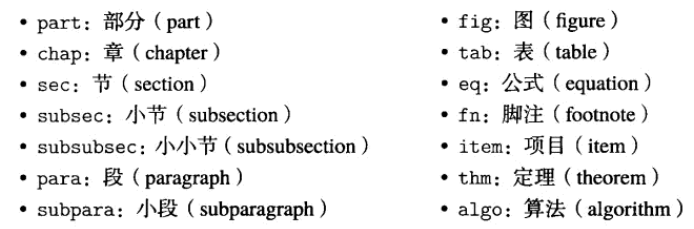
\includegraphics[width=\textwidth]{img//HowToName.png}
        \end{figure}
    \end{frame}
    
    \begin{frame}[fragile]
        \frametitle{pdf文件功能上的拓展}
        pdf文档支持很多特殊功能,如文档标签,超链接,电子表单等等,\LaTeX 也可以输出这样的功能,比如超链接,而这只需要添加一个宏包。
\begin{lstlisting}
% 在导言区(你最好不要忘了导言区是哪里)
% 插入下面的宏包
\usepackage{hyperref}
% 插入后,交叉引用会自动变为超链接。同样,至少编译两次
\end{lstlisting}
        \begin{itemize}
            \item 为刚才做的CrossReferences添加hyperref宏包,增加超链接
            \item 进入练习Hyperref中,猜测理解hypersetup中的内容。在pdf文件中,依次点击目录,公式标签,网页超链接,文件超链接,以及语句的链接。语句的链接可以注意一下,看看它是用了怎样的命令定位的。
        \end{itemize}
    \end{frame}



\subsection{索引}

    \begin{frame}[fragile]
    其实我觉得很多同学不知道什么叫索引。(快来打脸)
    \begin{figure}
    \centering
    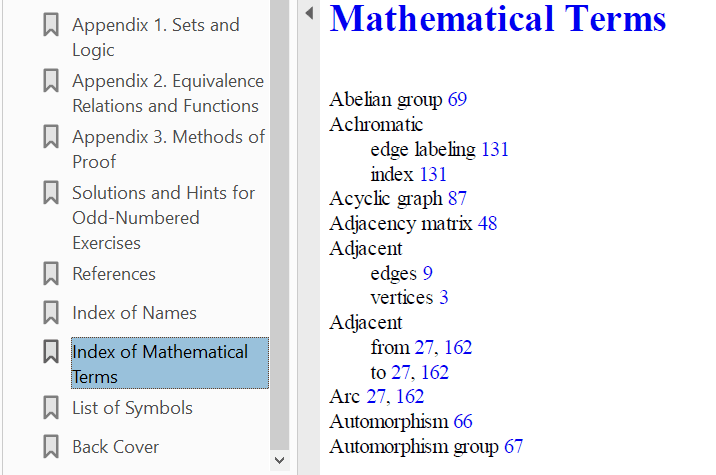
\includegraphics[width = 0.7\textwidth]{img//index.png}
    \end{figure}
    \end{frame}

    \begin{frame}[fragile]
    \frametitle{步骤}
    对tex文件,你需要做:
\begin{lstlisting}
导言区使用\makeindex
导言区调用makeidx宏包
需要索引的地方,使用\index{•}标记
在放索引的地方(通常是末尾),使用\printindex命令
\end{lstlisting}
    编译时,你需要:
\begin{lstlisting}
xelatex file_name
makeindex file_name
xelatex file_name
\end{lstlisting}
    注意:
    \begin{itemize}
        \item 配置好你的makeindex
        \item 不要忘了编译的次数和顺序
    \end{itemize}
    进入练习WordIndex,看看能不能编译出两个tex文件的索引
    \end{frame}

\subsection{文献引用}

    \begin{frame}[fragile]
        这块不细讲了,主要是编译的顺序
\begin{lstlisting}
xelatex filename
bibtex filename
xelatex filename
xelatex filename
\end{lstlisting}
         \begin{itemize}
             \item 在练习bib中按照上面的编译顺序,看看能否生成样例中的文件
             \item 在tex文件中用的指令,可去网上具体了解。
             \item 引用可以在tex文件中自己写,但用的比较多的是写在bib文件中(有专门的管理软件),最后导入,生成引用
         \end{itemize}
    \end{frame}




\section{其他}
    
    \begin{frame}[fragile]
        \frametitle{小建议}
        \begin{itemize}
            \item 要学会自学!自学!自学!
            \item 学会看错误日志(红色的那个),\textbf{耐下心来读英文}(其实不少人看到红色的字符串就不想认真读,然后自己肉眼挑BUG,或者问别人),自己解决不了的时候,一个很好的办法,是复制你的错误信息,以及你刚做的事的关键词(比如某个指令名),贴到搜索框搜索(当然是英文)\pause
             \item 对于上面这点,举个小例子:\verb|"!Undefined control sequence."|,这是一个伴随你一生的报错,绝大部分都可归为以下三种原因的一种:
                 \begin{itemize}
                     \item 拼错了!
                     \item 没导入宏包!
                     \item 用了不存在的指令!
                 \end{itemize}
        \end{itemize}
    \end{frame}
    
    \begin{frame}[fragile]{小建议}
        \begin{itemize}
            \item 另一位主讲人想要分享他昨晚(今天凌晨)的惨痛教训
            \item 遇到报错信息 \verb|Beamer - ! File ended while scanning use of \next|
            \item 尝试注释法肉眼找bug半小时无果
            \item 网上一查,错误原因是这样的
            \begin{figure}
                \centering
                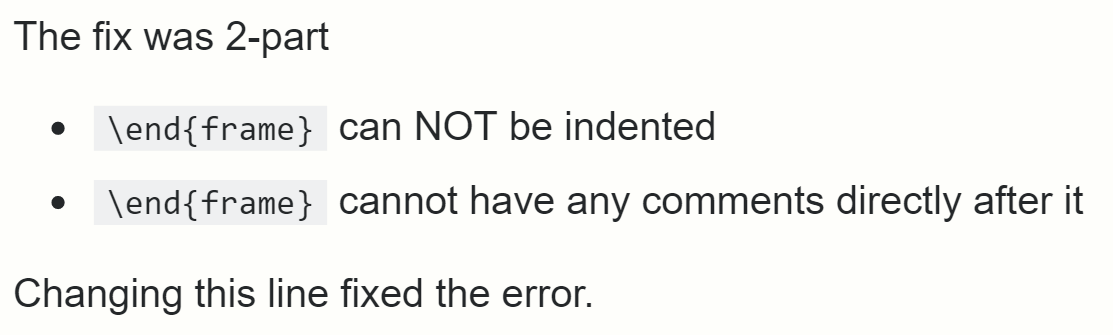
\includegraphics[width=.7\textwidth]{img/bug}
            \end{figure}
            \item 最后发现是在某个\verb|\end{frame}|后加了一个空格
        \end{itemize}
    \end{frame}
    
    \begin{frame}[fragile]
        \frametitle{小建议}
        \begin{itemize}
            \item 基础设施很重要!抽个时间,去专门学习你使用的编辑器是很有必要的。
            \item 关于上面这点,做些解释:
            \begin{itemize}
                \item 使用Tab键把你正在写的指令瞬间补全,也许就能省下百分之十的时间,积累起来就能让你多活一天!所以找个时间把常用的指令录进编辑器的代码补全里面是不是很有必要?(当然,花时间去网上找拓展包也是一样的)
                \item 再比如,自定义一个宏编译,设置为xelatex + bibtex + xelatex + xelatex,这样你按一个键就能完成引用的生成,是不是觉得很舒服?
                \item 夜晚看屏幕伤眼,心理也难受,所以换一个护眼又好看的主题皮肤是不是很好?
            \end{itemize}\pause
            \item 熟能生巧,可以渐渐用latex代替word去做平时的作业,可能一开始会有点慢,但当你渐渐熟悉自己的几个模板之后,速度就能反超word,还更好看
        \end{itemize}
    \end{frame}
    
    \begin{frame}[fragile]
        \begin{figure}
        
\includegraphics[width=0.45\textwidth]{img//tip.png}
        \end{figure}
        \begin{center}
        欢迎大家成为下一届学术软件教学系列讲座主讲人!
        \end{center}
    \end{frame}
    
    \begin{frame}[fragile]
        \frametitle{资源分享}
        \begin{itemize}
            \item \url{https://www.sharelatex.com/}
            \item \url{https://tex.stackexchange.com/}
            \item \url{http://tug.ctan.org/tex-archive/} 找文档,找手册!\\
            镜像站:\url{http://mirrors.ustc.edu.cn/CTAN/}
            \item \url{http://tug.org/}
        \end{itemize}
    \end{frame}
\end{document}
\end{lstlisting}
	\end{frame}

	\begin{frame}[fragile]
		\indent 划分文档的主要方式是\verb|\input{}|和\verb|\include{}|,将不同的章节内容写在不同的.tex文件中,用上述两种方式引入主文件中。\\
		\begin{description}
			\item[input] 相当于ctrl+c和ctrl+v,直接把代码复制过来,稳定、实用
			\item[include] 常和\verb|\includeonly|一起使用,可以选择性地编译子文件,常用于书籍之类的特大文档
		\end{description}
		\indent 两种方式的编译效果有细节上的不同,自己试试
	\end{frame}

	\begin{frame}
	截图来自stackexchange.com,题为input vs include
	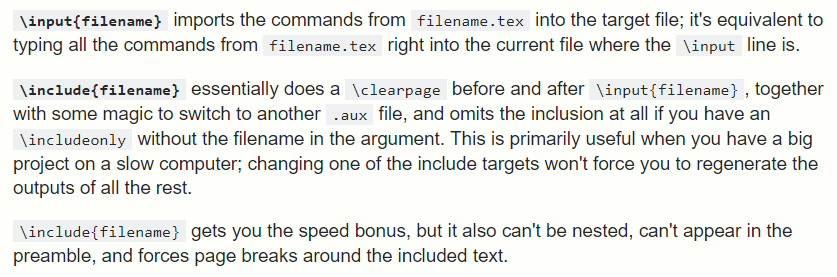
\includegraphics[width=\textwidth]{img//vs.png}	
	\end{frame}

	\begin{frame}[fragile]
		我们用的比较多的是input,当你觉得某一部分代码太长时,可以考虑写在别的.tex文件中,精简主文件,平时主要用在下面几种情况
		\begin{itemize}
			\item 导言区繁多的设置(通常会写在名为preamble的文件中,请看问求的作业模板)
			\item 异常庞大的表格
			\item 设置复杂的图片(比如需要使用很多子图subfig时)
		\end{itemize}
		此外可以去了解一下\verb|\endinput|的使用
	\end{frame}

\section{文本环境举隅}

\subsection{常用文本环境}

    \begin{frame}
    (其实会下面的就够了……)
    \begin{itemize}
        \item 文本环境:quote, quotation, abstarct(写诗的同学可以去了解verse)
        \item 列表环境:itemize, enumerate
        \item 定理类环境:thm, lemma, definition, proof
        \item 抄录和代码环境:verb, lstlisting
        \item 脚注:footnote
    \end{itemize}
    \end{frame}
    
    \begin{frame}
    \frametitle{练习和小建议}
    \begin{itemize}
    \item 打开练习list, theorem, listing$\_$code, page
    \item 想要用好文本环境,更建议看手册而不是上网搜索
    \end{itemize}
    \end{frame}
\section{中文支持}
\subsection{了解\CTeX}
\begin{frame}{How to get Chinese document?}{\CTeX}
	\CTeX 是最新的也是最便利的\LaTeX 中文支持的开源项目,可以参考其\href{material/LM/CTEXmanual.pdf}{\textcolor{blue}{使用手册}}。
	\begin{itemize}
		\item 全面汉化
		\item 更智能的排版
		\item 强大的自定义设置
	\end{itemize}
	一般使用默认设置即可,有特殊需求可翻阅手册作适当调整。
\end{frame}
\begin{frame}
	\begin{table}\caption{\CTeX 宏集的组成}
		\footnotesize
		\begin{tabular}{llp{6cm}}
			\toprule
			类别 & 文件 & 说明 \\
			\midrule
			文档类 & ctexart.cls & 标准文档类article 的汉化版本,一般适用于短篇幅的文章\\
			& ctexrep.cls & 标准文档类report 的汉化版本,一般适用于中篇幅的报告\\
			& ctexbook.cls & 标准文档类book 的汉化版本,一般适用于长篇幅的书籍\\
			& ctexbeamer.cls & 文档类beamer 的汉化版本,适用于幻灯片演示\\
			\midrule
			宏包 & ctex.sty & 提供全部功能,但默认不开启章节标题设置功能,需要使用heading 选项来开启\\
			& ctexsize.sty & 定义和调整中文字号,在ctex 宏包或CTEX 中文文档类之外单独调用\\
			& ctexheading.sty & 提供章节标题设置功能,在ctex 宏包或CTEX 中文文档类之外单独调用\\
			\bottomrule
		\end{tabular}
	\end{table}
\end{frame}
\begin{frame}[fragile]
	\begin{itemize}
		\item 文档类
\begin{lstlisting}
\documentclass{ctexart}
\documentclass{ctexrep}
\documentclass{ctexbook}
\documentclass{ctexbeamer}
\end{lstlisting}		
		\item 宏包
\begin{lstlisting}
\usepackage{ctex}
\usepackage{ctexsize}      
\usepackage{ctexheading}   
\end{lstlisting}
	\end{itemize}
	\vspace{2ex}
	\textcolor{red}{注意}:\texttt{ctexcap} 是默认打开 \texttt{heading} 选项的 \texttt{ctex} 宏包,手册中明确说明其为过时宏包!
\end{frame}
\begin{frame}
	两个最常用选项\texttt{heading}与\texttt{scheme}。

	打开\texttt{ctex.tex},体会不同选项的区别。
	\begin{itemize}
		\item \texttt{ctexart}类文档与\texttt{ctex}宏包的默认选项都是\texttt{heading=true,scheme=chinese}
		\item \texttt{heading=false,scheme=plain}相当于只是支持中文,所有的版式都还是英文的
		\item 如果觉得标题居中太蠢了想要靠左,可以用\texttt{heading=false}(\texttt{scheme=chinese}是默认选项不用改)
	\end{itemize}
\end{frame}
\section{强大的数学公式}
\begin{frame}[fragile]{写在前面}
	除了一些最简单的数学公式,大部分都需要宏包支持。建议平时需要输入公式时就直接使用以下四个宏包
\begin{lstlisting}
\usepackage{amsmath,amsfonts,amssymb,mathtools}
\end{lstlisting}
	这能够支持大多数的数学公式,而不必去纠结什么时候应该用哪一个、哪一个是多余的。

	\vspace{2ex}
	在讨论更多的数学环境前,我们统一使用 \cprotect\fbox{\verb|$|$\dots$\verb|$|} 输入行内(inline)公式,\cprotect\fbox{\verb|\[|$\dots$\verb|\]|} 输入行间(displayed)公式。

	\vspace{2ex}
	\textcolor{red}{注意}:凡是要用到数学字符的地方必须进入数学环境,有些字符虽然不在数学环境下也能输入,但是区别很大!
	\begin{table}
		\begin{tabular}{rlrl}
			\textrm{1+1=2} & $1+1=2$ \quad & \quad \textrm{a sin x} & $a \sin x$
		\end{tabular}
	\end{table}
\end{frame}

\subsection{数学符号}
\begin{frame}[fragile]{字母表与数学字体}
	在公式环境内默认使用 \cprotect\fbox{\verb|\mathnormal|} 字体,与正文环境下默认字体对比如下
	\begin{itemize}
		\item Capital
		\begin{itemize}
			\item \textrm{ABCDEFGHIJKLMNOPQRSTUVWXYZ}
			\item $ABCDEFGHIJKLMNOPQRSTUVWXYZ$
		\end{itemize}
		\item Lower case
		\begin{itemize}
			\item \textrm{abcdefghijklmnopqrstuvwxyz}
			\item $abcdefghijklmnopqrstuvwxyz$
		\end{itemize}
	\end{itemize}
	其明显特征是斜体且间距较正文大一些。

	\vspace{2ex}
	而\cprotect\fbox{\verb|\mathit|}, \cprotect\fbox{\verb|\mathrm|}, \cprotect\fbox{\verb|\mathbf|}, \cprotect\fbox{\verb|\mathsf|}, \cprotect\fbox{\verb|\mathtt|} 这些数学字体通常直接使用相对应的正文字体\cprotect\fbox{\verb|\text**|}。
\end{frame}
\begin{frame}[fragile]{选用正确的字体}
	\begin{itemize}
		\item 变量使用默认字体,如$x, y, z$
		\item $\mathrm{e}, \mathrm{i}$等常量应使用罗马体 \cprotect\fbox{\verb|\mathrm|}
		\item 集合$\mathbb{N}, \mathbb{R}$等可使用 \verb|amssymb|提供的黑板粗体 \cprotect\fbox{\verb|\mathbb|}
		\item 向量$\bm{v}$应加粗,实现方法有很多,这里推荐 \verb|bm| 宏包的 \cprotect\fbox{\verb|\bm|} 命令
	\end{itemize}
\end{frame}
\begin{frame}[fragile]{希腊字母}
	\begin{itemize}
		\item 小写希腊字母
		\begin{itemize}
			\item 一般 \cprotect\fbox{\verb|\+小写拼写|},如 \cprotect\fbox{\verb|\alpha|} 即输出$\alpha$
			\item 注意$\mu, \nu$分别为 \cprotect\fbox{\verb|\mu|},\cprotect\fbox{\verb|\nu|}
			\item 一部分希腊字母有变体,这些变体在数学公式中常常用到,只需在前面加上 \verb|var|
				\begin{itemize}
				\item[] \small $\epsilon \rightarrow \varepsilon$ \qquad $\phi \rightarrow \varphi$ \qquad
					$\theta \rightarrow \vartheta$ \qquad $\sigma \rightarrow \varsigma$ \qquad
					$\pi \rightarrow \varpi$
				\end{itemize}
		\end{itemize}
		\item 大写希腊字母
		\begin{itemize}
			\item 一部分大写希腊字母与拉丁字母形状相同,直接使用即可,如$\mathrm{A, B}$
			\item 将小写希腊字母输入时首字母大写即可得到其大写形式,如 \cprotect\fbox{\verb|\Gamma|} 得到$\Gamma$
			\item 大写希腊字母一般用正体,前面加 \cprotect\fbox{\verb|var|} 或使用 \cprotect\fbox{\verb|\mathnormal|} 可得到倾斜形式
		\end{itemize}
		\item 小写希腊字母直立体形式?
		\begin{itemize}
			\item 数字字体宏包 \verb|upgreek|,在前面加上 \cprotect\fbox{\verb|up|}
			\item \cprotect\fbox{\verb|\pi|} $\rightarrow$ \cprotect\fbox{\verb|\uppi|} \qquad $\pi \rightarrow \uppi$
		\end{itemize}
	\end{itemize}
\end{frame}
\begin{frame}[fragile]{常用符号}
	\begin{table}\caption{数学普通符号(部分)}
		\begin{tabular}{llllll}
			\toprule
			$\hbar$ & \verb|\hbar| & $\ell$ & \verb|\ell| & $\partial$ & \verb|\partial| \\
			$\infty$ & \verb|\infty| & $\prime$ & \verb|\prime| & $\emptyset$ & \verb|\emptyset| \\
			$\nabla$ & \verb|\nabla| & $\forall$ & \verb|\forall| & $\exists$ & \verb|exists| \\
			$\neg$ & \verb|\neg| & $\varnothing$ & \verb|\varnothing| & $\angle$ & \verb|\angle| \\
			$\clubsuit$ & \verb|\clubsuit| & $\diamondsuit$ & \verb|\diamondsuit| & $\heartsuit$ & \verb|\heartsuit| \\
			$\spadesuit$ & \verb|\spadesuit| & $\triangle$ & \verb|\triangle| & $\square$ & \verb|\square| \\
			$\flat$ & \verb|\flat| & $\natural$ & \verb|\natural| & $\sharp$ & \verb|\sharp|\\
			\bottomrule
		\end{tabular}
	\end{table}
\end{frame}
\begin{frame}[fragile]{常用符号}
	\begin{table}\caption{可同时用在文本和数学模式中的符号}
		\begin{tabular}{llllllll}
			\toprule
			$\#$ & \verb|\#| & $\&$ & \verb|\&| & $\%$ & \verb|\%| & $\$$ & \verb|\$| \\
			$\_$ & \verb|\_| & $\{$ & \verb|\{| & $\}$ & \verb|\}| & & \\
			$\P$ & \verb|\P| & $\S$ & \verb|\S| & $\dag$ & \verb|\dag| & $\ddag$ & \verb|\ddag| \\
			$\copyright$ & \verb|\copyright| & $\pounds$ & \verb|\pounds| & $\ldots$ & \verb|\ldots| & & \\
			$\checkmark$ & \verb|\checkmark| & $\circledR$ & \verb|\circledR| & $\maltese$ & \verb|\maltese| & $\yen$ & \verb|\yen| \\
			\bottomrule
		\end{tabular}
	\end{table}
	\begin{table}\caption{希伯来字母}
		\begin{tabular}{llllllll}
			\toprule
			$\aleph$ & \verb|\aleph| & $\beth$ & \verb|\beth| & $\daleth$ & \verb|\daleth| & $\gimel$ & \verb|\gimel| \\
			\bottomrule
		\end{tabular}
	\end{table}
\end{frame}
\begin{frame}[fragile]{数学算子}{Math operator}
	\begin{itemize}
		\item 巨算符(large operator)
		\begin{itemize}
			\item 所谓巨算符是大小可变的运算符
			\item 其在行内与行间大小是不同的
			\item 一般可以添加有上下标(数学结构中会讲)
			\item 行内行间上下标的形式也有所不同
		\end{itemize}
	\end{itemize}
	\begin{align*}
		\int_a^b & \textstyle \int_a^b & \iint_m^n & \textstyle \iint_m^n & \oint_{|z|=1} & \textstyle \oint_{|z|=1} \\
		\sum_{n=0}^{\infty} & \textstyle \sum_{n=0}^{\infty} & \prod_{1 \le i < j \le n} & \textstyle \prod_{1 \le i < j \le n} & \bigcup\nolimits_{i=1}^{n} & \textstyle \bigcup\limits_{i=1}^{n}
	\end{align*}
	\small \quad \cprotect\fbox{\verb|\limits|} \quad \cprotect\fbox{\verb|\nolimits|} \quad 行内公式尽量避免上下限放在算符上下位置
\end{frame}
\begin{frame}[fragile]{数学算子}{Math operator}
	\begin{itemize}
		\item 文字名称的算子
		\begin{itemize}
			\item 使用直立罗马体排印,一般 \cprotect\fbox{\verb|\+名称|} 即可
			\item 分为两类,带上下限的与不带上下限的
			\begin{itemize}
				\item $\log \quad \sin \quad \cosh \quad \arctan \quad \exp$ 
				\item $\lim \quad \max \quad \min \quad \sup \quad \inf$ 
			\end{itemize}
			\item 带上下限的算子使用起来与巨算符相似\\
				\qquad $\lim\limits_{x \to 0} \qquad \lim_{x \to 0}$
			\item 如果需要定义新的算子,可以在导言区使用 \verb|\DeclareMathOperator(*)|,带 \verb|*|表示带上下限
			\begin{itemize}
				\item \verb|\DeclareMathOperator{\arccot}{arccot}| \\ $\arccot$
				\item \verb|\DeclareMathOperator{\sign}{sgn}| \\ $\sign$
				\item \verb|\DeclareMathOperator*{\limsup}{lim\,sup}| \\ $\limsup$
			\end{itemize}
		\end{itemize}
	\end{itemize}
\end{frame}
\begin{frame}[fragile]{二元运算符与关系符}
	\begin{itemize}
		\item $\cprotect\overset{\cprotect\fbox{\scriptsize\verb|+|}}{+}, 
	\cprotect\underset{\cprotect\fbox{\scriptsize\verb|-|}}{-}, 
	\cprotect\overset{\cprotect\fbox{\scriptsize\verb|\times|}}{\times}, 
	\cprotect\underset{\cprotect\fbox{\scriptsize\verb|\div|}}{\div}$等二元运算符与
	$\cprotect\overset{\cprotect\fbox{\scriptsize\verb|=|}}{=}, 
	\cprotect\underset{\cprotect\fbox{\scriptsize\verb|>|}}{>}, 
	\cprotect\overset{\cprotect\fbox{\scriptsize\verb|<|}}{<}, 
	\cprotect\underset{\cprotect\fbox{\scriptsize\verb|\ne|}}{\ne}, 
	\cprotect\overset{\cprotect\fbox{\scriptsize\verb|\le|}}{\le}$\textrm{,} $
	\cprotect\underset{\cprotect\fbox{\scriptsize\verb|\ge|}}{\ge}$\textrm{,} $
	\cprotect\overset{\cprotect\fbox{\scriptsize\verb|\ll|}}{\ll}$\textrm{,} $
	\cprotect\underset{\cprotect\fbox{\scriptsize\verb|\gg|}}{\gg}$等关系符与前后变量之间会保留一定的空隙,且行内公式可以在它们的后面断行。
	\item 二元关系符数量庞大,除了一些最常用的,一般有需要的时候随用随查即可。
	\item 使用 \cprotect\fbox{\verb|\mathbin|} 和 \cprotect\fbox{\verb|\mathrel|} 可以将其参数当作二元运算符和二元关系符来对待,可用于定义新运算或一些其他用途。
	\item 箭头符号与逻辑符号使用时同样可以查阅,不再赘述。
	\end{itemize}
\end{frame}
\begin{frame}[fragile]{定界符}
	\[\{\frac{\partial y_j}{\partial x_i} | i=1,2,\cdots,n,\, j=1,2,\cdots,m\}\]
	\[\left\{\frac{\partial y_j}{\partial x_i} \middle| i=1,2,\cdots,n,\, j=1,2,\cdots,m\right\}\]
	上例中的$\{\,|\,\}$均为定界符,其大小可以根据式子的大小而改变。
	\begin{itemize}
		\item 括号定界符
		\[(\,)\quad[\,]\quad\{\,\}\quad\langle\,\rangle\quad\lfloor\,\rfloor\quad\lceil\,\rceil\]
		\item 非括号定界符
		\[/\quad\backslash\quad|\quad\|\]
		\item 输入
		\begin{itemize}
			\item \verb|( ) [ ] \{ \} \langle \rangle|\\
				\verb|\lfloor \rfloor \lceil \rceil|
			\item \verb!/ \backslash | \|!
		\end{itemize}
	\end{itemize}
\end{frame}
\begin{frame}[fragile]{如何确定定界符大小}
	\begin{itemize}
		\item 自动调整
		\begin{itemize}
			\item 使用 \cprotect\fbox{\verb|\left( ... \right)|},左右必须成对出现
			\item 如果只需要一个定界符,可以用 \cprotect\fbox{\verb|.|} 表示空的定界符,如 \cprotect\fbox{\verb|\left.|}
			\item 需要三个定界符的话可使用 \cprotect\fbox{\verb|\middle|} 放在中间,如前例
		\end{itemize}
		\item 手动调整
		\begin{itemize}
			\item 提供了 \cprotect\fbox{\verb|\big|},\cprotect\fbox{\verb|\Big|}, \cprotect\fbox{\verb|\bigg|},\cprotect\fbox{\verb|\Bigg|} 四种大小供手动调节
			\item 可以在后面加上 \cprotect\fbox{\verb|l m r|} 配套使用
			\item 自动调整效果不理想时,可以试试手动调整
			\item 在明确“左右”(如 \cprotect\fbox{\verb|\left \right|} 或 \cprotect\fbox{\verb|\Bigl \Bigr|})时,可直接使用 \cprotect\fbox{\verb|<>|} 表示尖括号而不致与$<>$混淆
		\end{itemize}
	\end{itemize}
\end{frame}
\begin{frame}[fragile]{标点符号}
	\begin{itemize}
		\item 数学环境内应使用英文标点,否则会报错
		\item 常用的标点符号有$, \quad ; \quad ! \quad ? \quad \colon$
		\item 应注意的是\cprotect\fbox{\verb|:|}是作为二元关系符存在的(如$f(x):=x, \{x : x>0\}$),而作为标点的冒号是 \cprotect\fbox{\verb|\colon|},其两侧间距不同,表示比例时则最好用 \cprotect\fbox{\verb|\mathbin{:}|}
		\item 省略号有很多种,在矩阵中常用到,平时最常用的是 \cprotect\fbox{\verb|\cdots|} $\cdots$ 和 \cprotect\fbox{\verb|\ldots|} $\ldots$ (或直接使用 \cprotect\fbox{\verb|\dots|} 让latex自己选择)
		\item 标点后是无法换行的,像$f(x,y,z)$谁也不希望在中间断行,而$a_1$\textrm{,} $a_2$\textrm{,} $a_3$\textrm{,} $\cdots$\textrm{,} $a_n$希望能断行时应将标点置于数学环境之外并加上空格
		\item 数学环境中空格不起作用,但可以分隔各部分让公式结构更清晰
	\end{itemize}
\end{frame}

\subsection{数学结构}
\begin{frame}[fragile]{上下标}
	\begin{itemize}
		\item 上标用 \verb|^| 表示,下标用 \verb|_| 表示
		\item 超过一个字符时就应使用$\{\,\}$
		\item \verb|'| 是一种特殊的上标,相当于 \cprotect\fbox{\verb|^\prime|}
		\item 使用 \cprotect\fbox{\verb|\overset|} 和 \cprotect\fbox{\verb|\underset|}可以在任意符号上下方添加标记
	\end{itemize}
\end{frame}
\begin{frame}[fragile]{分式}
	\begin{itemize}
		\item 使用 \cprotect\fbox{\verb|\frac{num}{den}|} 输入分式,先输入分子(numerator),后输入分母(denominator)
		\item 行内默认使用正文格式(text style)分式,行间默认使用显示格式(display style)分式,可以使用 \cprotect\fbox{\verb|\tfrac|} 与 \cprotect\fbox{\verb|\dfrac|} 指定使用某一种
		\item 行内使用分式时,$a/b$效果往往比$\frac ab$更好
		\item 连分式用 \cprotect\fbox{\verb|\cfrac|},这里不细讲
		\item 顺带一提,\cprotect\fbox{\verb|\textstyle|} 和 \cprotect\fbox{\verb|\displaystyle|} 可以指定整条公式以哪种方式显示
	\end{itemize}
\end{frame}
\begin{frame}[fragile]{根式}
	\begin{itemize}
		\item \cprotect\fbox{\verb|\sqrt[root]{arg}|}
		\item \texttt{[\,]}内为可选项,用\cprotect\fbox{\verb|\uproot|} 与 \cprotect\fbox{\verb|\leftroot|} 可以微调\texttt{root}位置,参数为整数
		\item 被开方数不是整数或结构复杂时,通常改用等价的指数形式
		\item 使用 \cprotect\fbox{\verb|\vphantom|} 占位来获得统一的高度\\[1ex]
		\verb|\sqrt{\frac 12} < \sqrt{\vphantom{\frac12}2}|
		\[\sqrt{\frac 12} < \sqrt{\vphantom{\frac12}2}\]
		\item \cprotect\fbox{\verb|\mathstrut|} 用来平衡不同高度和深度的字母\\[1ex]
		\verb|\sqrt b \sqrt y|\\
		\verb|\sqrt{\mathstrut b} \sqrt{\mathstrut y}|
		\[\sqrt b \sqrt y \quad \rightarrow \quad \sqrt{\mathstrut b} \sqrt{\mathstrut y}\]
	\end{itemize}
\end{frame}
\begin{frame}[fragile]{矩阵}
	\begin{itemize}
		\item 输入矩阵结构需要矩阵环境,它们的区别在于外面的括号不同
		\begin{itemize}
			\item \texttt{ matrix}环境 \quad 无括号
			\item \texttt{pmatrix}环境 \quad 圆括号
			\item \texttt{bmatrix}环境 \quad 方括号
			\item \texttt{Bmatrix}环境 \quad 大括号
			\item \texttt{vmatrix}环境 \quad 单竖线
			\item \texttt{Vmatrix}环境 \quad 双数线
		\end{itemize}
		\item 以一个最简单的二阶矩阵为例\\
		\begin{minipage}[c]{0.5\textwidth}
\begin{lstlisting}
\[ \begin{pmatrix}
       a_{11} & a_{12} \\
       a_{21} & a_{22}
   \end{pmatrix} \]
\end{lstlisting}
		\end{minipage}
		\begin{minipage}[c]{0.4\textwidth}
			\[ \begin{pmatrix}
				a_{11} & a_{12} \\
				a_{21} & a_{22}
			\end{pmatrix} \]
		\end{minipage}
	\end{itemize}
\end{frame}
\subsection{数学环境}
\begin{frame}[fragile]{概述}
	我们先前使用的 \cprotect\fbox{\verb|\[|$\dots$\verb|\]|} 实质是
\begin{lstlisting}
\begin{equation*}
    ...
\end{equation*}
\end{lstlisting}
	的缩写,其中“$*$”表示不给该公式标序。

	\vspace{2ex}
	出于各方面的需求,我们并不满足于这样一个简单居中、无法换行的数学环境,而是会有诸多其他方面的要求。这时我们需要更多的数学环境来提供支持。
\end{frame}
\begin{frame}[fragile]{多行公式}{每行均为一个公式}
	\begin{itemize}
		\item 简单的多个公式罗列: \verb|gather(*)|
		\begin{itemize}
			\item 每行公式都是居中显示的
			\item 使用 \cprotect\fbox{\verb|\\|} 换行
			\item 某行不需要编号,在 \cprotect\fbox{\verb|\\|} 前加  \cprotect\fbox{\verb|\notag|} 
		\end{itemize}
		\item 公式按关系符对齐: \verb|align(*)|
		\begin{itemize}
			\item 使用 \cprotect\fbox{\verb|\\|} 换行,关系符前加 \cprotect\fbox{\verb|&|} 表示对齐
			\item \cprotect\fbox{\verb|&|} 一般放在二元关系符($=,<,>$等)前面
			\item 有时可巧用 \cprotect\fbox{\verb|\phantom|} 变通 
		\end{itemize}
		\item 多行公式每行都会产生一个编号,不希望产生的话可以使用\cprotect\fbox{\verb|\notag|}
	\end{itemize}
\end{frame}
\begin{frame}
	练习:尝试输出以下公式。

	\begin{minipage}{0.95\textwidth}
	\begin{gather}
		\partialratio{A}{x}{y} = \lim_{\Delta x \to 0} \frac{f(x+\varDelta x,y)-f(x,y)}{\varDelta x} \\
		\partialratio{A}{y}{x} = \lim_{\Delta y \to 0} \frac{f(x,y+\varDelta y)-f(x,y)}{\varDelta y}
	\end{gather}
	\hrule
	\begin{align}
		& \mathrel{\phantom{=}} (a + b)(a^2 - ab + b^2)\notag \\
		& = a^3 - a^2b + ab^2 + a^2b - ab^2 + b^3\notag \\
		& = a^3 + b^3
	\end{align}
	\end{minipage}
\end{frame}
\begin{frame}[fragile]{多行公式}
	\begin{itemize}
		\item \verb|align(*)| 的另一个用处:排版多列公式
		\begin{itemize}
			\item 每行的基本格式
			\begin{itemize}
				\item[] \verb|a &= b  &  c &= d  &  e &= f \\|
			\end{itemize}
			\item 最后一行不需要 \cprotect\fbox{\verb|\\|}
			\item 按照行来标序
			\item \cprotect\fbox{\verb|&|} 必然为奇数个,出现偶数个会报错(为什么?)
		\end{itemize}
		\item 关于 \verb|flalign(*)|
		\begin{itemize}
			\item 与 \verb|align(*)| 是类似的
			\item 会把多列公式水平方向分散对齐
		\end{itemize}
		\item 关于 \verb|alignat(*)|
		\begin{itemize}
			\item 与 \verb|align(*)| 也是类似的
			\item 不会主动产生间距,需要手动输入间距大小
			\item 需要一个参数表示每行要对齐的公式个数
		\end{itemize}
	\end{itemize}
\end{frame}
\begin{frame}[fragile]
	对比 \verb|align(*)| 与 \verb|flalign(*)|

	\vspace{2ex}
	\clean
	\begin{minipage}{0.49\textwidth}
		\begin{itemize}
			\item 使用 \verb|align|
			\begin{align}
				x + y &= 2 & x &= 1 \\
				x - y &= 0 & y &= 1
			\end{align}
		\end{itemize}
	\end{minipage}
	\clean
	\begin{minipage}{0.49\textwidth}
		\begin{itemize}
			\item 使用 \verb|flalign|
			\begin{flalign}
				x + y &= 2 & x &= 1 \\
				x - y &= 0 & y &= 1
			\end{flalign}
		\end{itemize}
	\end{minipage}

	\vspace{3ex}
	巧用 \verb|alignat|(使用 \verb|align|必须借助 \cprotect\fbox{\verb|\phantom|})

	\begin{minipage}{0.69\textwidth}
\begin{lstlisting}
\begin{alignat*}{5}
    &1 & &+2 & &+3 & &+4 & &=10 \\
    &1 & &   & &+3 & &   & &=4 \\
    &  & &+2 & &   & &+4 & &=6
\end{alignat*}
\end{lstlisting}			
	\end{minipage}
	\begin{minipage}{0.29\textwidth}
		\begin{alignat*}{5}
			&1 & &+2 & &+3 & &+4 & &=10 \\
			&1 & &   & &+3 & &   & &=4 \\
			&  & &+2 & &   & &+4 & &=6
		\end{alignat*}
	\end{minipage}
\end{frame}
\begin{frame}[fragile]{多行公式}
	\begin{itemize}
		\item 如何在多行公式之间插入说明性文字?
		\begin{itemize}
			\item 每次都退出数学环境输入文字过于麻烦
			\item 退出数学环境会破环上下公式间对齐关系
		\end{itemize}
		\item \cprotect\fbox{\verb|\text|} 行内插入文字
		\item \cprotect\fbox{\verb|\intertext|} 换行顶格插入文字(前一行的 \cprotect\fbox{\verb|\\|} 可省略)
		\item \cprotect\fbox{\verb|\shortintertext|} 提供更为紧凑的行间距
	\end{itemize}
\end{frame}
\begin{frame}
	例:

	\vspace{2ex} \clean
	绝热过程中,$Q=0$,不做非膨胀功时,有
	\begin{gather}
		\di U = \delta W
		\quad \text{或} \quad
		\di U + p \di V = 0
		\shortintertext{已知}
		\todi{U}{T}{V}
		\shortintertext{对理想气体,}
		\di U = C_V \di T, \quad \Delta U = \int_{T_1}^{T_2}C_V \di T
		\intertext{若$C_V$为常数,}
		\Delta U = C_V(T_2-T_1) = W
	\end{gather}
\end{frame}
\begin{frame}[fragile]{多行公式}
	\begin{itemize}
		\item 多个联系紧密的公式如何共用一个编号?
		\begin{itemize}
			\item[] 使用 \verb|subequations| 环境
		\end{itemize}
		\item 示例:
\begin{lstlisting}
\begin{subequations}
\begin{align}
  a \cdot b &= b \cdot a \\
  (a \cdot b) \cdot c &= a \cdot (b \cdot c) \\
  a \cdot (b + c) &= a \cdot b + a \cdot c 
\end{align}
\end{subequations}
\end{lstlisting}
		\clean \vspace{-0.5cm}
		\begin{minipage}{0.7\textwidth}
			\begin{subequations}
				\begin{align}
					a \cdot b &= b \cdot a \\
					(a \cdot b) \cdot c &= a \cdot (b \cdot c) \\
					a \cdot (b + c) &= a \cdot b + a \cdot c 
				\end{align}
			\end{subequations}
		\end{minipage}
	\end{itemize}
\end{frame}
\begin{frame}
练习:尝试输出如下的麦克斯韦方程组。

	\vspace{2ex} \clean
\begin{minipage}[t]{0.54\textwidth}
	\begin{itemize}
		\item 积分形式
	\end{itemize}
\end{minipage}
\quad
\begin{minipage}[t]{0.4\textwidth}
	\begin{itemize}
		\item 微分形式
	\end{itemize}
\end{minipage}
\begin{minipage}[c]{0.54\textwidth}
	\begin{subequations}
		\begin{align}
			\varoiint_S \bm{D} \cdot \di \bm{S} &= q, \\
			\varoiint_S \bm{B} \cdot \di \bm{S} &= 0, \\
			\oint_L \bm{E} \cdot \di \bm{\ell} &= - \iint \frac{\partial \bm{B}}{\partial\, t} \cdot \di \bm{S}, \\
			\oint_L \bm{H} \cdot \di \bm{\ell} &= I_0 + \iint \frac{\partial \bm{D}}{\partial\, t} \cdot \di \bm{S}.
		\end{align}
	\end{subequations}
\end{minipage}
\quad
\begin{minipage}[c]{0.4\textwidth}
	\begin{subequations}
		\begin{align}
			\nabla \cdot \bm{D} &= \rho_f, \\
			\nabla \cdot \bm{B} &= 0, \\
			\nabla \times \bm{E} &= -\frac{\partial \bm{B}}{\partial\, t}, \\
			\nabla \times \bm{H} &= \bm{J}_f + \frac{\partial \bm{D}}{\partial\, t}.
		\end{align}
		\end{subequations}		
	\end{minipage}
\end{frame}
\begin{frame}{拆分公式}{整体为一个公式}
	行内公式中,对于长公式如$1+2+3+4+5+6+7+8+9+10+11+12+13+14+15+16+17+18+19+20+21+22+23+24+25+26+27+28+29+30$我们先前提过是可以在二元运算符后换行的,但是对于行间公式则不然,见下例。
	\[
	1+2+3+4+5+6+7+8+9+10+11+12+13+14+15+16+17+18+19+20+21+22+23+24+25+26+27+28+29+30
	\]
	这时候可以使用\texttt{multline(*)}环境。(注意不是 \textcolor{red}{\texttt{multiline}}!)
\end{frame}
\begin{frame}[fragile]
\begin{lstlisting}
\begin{multline}
    1+2+3+4+5+6+7 \\
    +8+9+10+11+12+13 \\
    +14+15+16+17+18+19+20+21 \\
    +22+23+24+25 \\
    +26+27+28+29+30
\end{multline}
\end{lstlisting}
	\clean
	\begin{multline}
		1+2+3+4+5+6+7 \\
		+8+9+10+11+12+13 \\
		+14+15+16+17+18+19+20+21 \\
		+22+23+24+25 \\
		+26+27+28+29+30
	\end{multline}
\end{frame}
\begin{frame}[fragile]{拆分公式}
	\begin{itemize}
		\item 可以看出\texttt{multline}环境中首行是左对齐的,尾行是右对齐的,中间行则是居中
		\item 公式的左右边距是通过长度变量\cprotect\fbox{\verb|\multlinegap|} 和 \cprotect\fbox{\verb|\multlinetaggap|} 设置的
		\item \cprotect\fbox{\verb|\shoveleft{}|} 和 \cprotect\fbox{\verb|\shoveright{}|} 可设置中间行像首尾两行那样左/右对齐
	\end{itemize}
	\setlength{\multlinegap}{4em}
	\setlength{\multlinetaggap}{4em}
	\begin{multline*}
		1+2+3+4+5+6+7 \\
		\shoveright{+8+9+10+11+12+13} \\
		+14+15+16+17+18+19+20+21 \\
		\shoveleft{+22+23+24+25} \\
		+26+27+28+29+30
	\end{multline*}
\end{frame}
\begin{frame}[fragile]
\begin{lstlisting}
\setlength{\multlinegap}{4em}
\setlength{\multlinetaggap}{4em}
\begin{multline*}
    1+2+3+4+5+6+7 \\
    \shoveright{+8+9+10+11+12+13} \\
    +14+15+16+17+18+19+20+21 \\
    \shoveleft{+22+23+24+25} \\
    +26+27+28+29+30
\end{multline*}
\end{lstlisting}
\end{frame}
\begin{frame}[fragile]{拆分公式}
	\begin{itemize}
		\item 如果想要在等号处对齐,可以考虑\texttt{split}环境
		\item \texttt{split}环境应当内嵌于\texttt{equation}中,使用方法上与\texttt{align}等类似
	\end{itemize}
	\clean
	\begin{minipage}{0.43\textwidth}
\begin{lstlisting}
\begin{equation}
\begin{split}
(AB)(B^{-1}A^{-1}) 
&= A(BB^{-1})A^{-1} \\
&= AIA^{-1} 
 = AA^{-1} \\
&= I
\end{split}
\end{equation}
\end{lstlisting}
	\end{minipage}
	\begin{minipage}{0.56\textwidth}
		\begin{equation} \begin{split}
			(AB) (B^{-1}A^{-1}) &= A(BB^{-1})A^{-1} \\
			&= AIA^{-1} = AA^{-1} \\
			&= I
		\end{split} \end{equation}
	\end{minipage}
\end{frame}
\begin{frame}[fragile]{组合成块}
	如何输入分段函数,如
	\[ \sign x = \begin{cases}
	1, & x > 0, \\
	0, & x = 0, \\
	-1, & x < 0.
	\end{cases} \]

	使用\texttt{cases} 环境(同样需要内嵌在\texttt{equation}等环境中)。
\begin{lstlisting}
\[ \sign x = \begin{cases}
  1, & x > 0, \\
  0, & x = 0, \\
  -1, & x < 0.
\end{cases} \]
\end{lstlisting}
\end{frame}

\begin{frame}{组合成块}
	\begin{itemize}
		\item 使用\texttt{dcases}环境得到显示格式大小的公式
		\item 此外使用上述部分环境的\texttt{+ed}模式能得到更多的将公式组合成块的应用
		\begin{itemize}
	 		\item 如:\texttt{gathered}, \texttt{aligned}, \texttt{alignedat}, \texttt{multilined}
	 		\item \texttt{lgathered}与\texttt{rgathered}可以设置环境内的若干行公式左对齐或右对齐,配合定界符使用
	 	\end{itemize}
	 	\item 以上环境的使用方法不变,它们都将多行的公式组合成块放在了一个公式环境内
	 	\item 这里只举几个例子,请自行融会贯通
	\end{itemize}
	\centering
	\texttt{请打开文件equation.tex并编译。}
\end{frame}
\section{图表与浮动体}

\subsection{构建表格}
\begin{frame}{tabular与array}
	\begin{itemize}
		\item tabular主要用于文本环境(数学模式下也可使用,但是还是按照文本模式排版)
		\item array用在数学环境中,主要用于排版复杂矩阵等包含数学符号的公式
		\item 二者用法上是相似的,这里只讲tabular
	\end{itemize}
\end{frame}
\begin{frame}[fragile]{基本格式}
\begin{lstlisting}
\begin{tabular}[<垂直对齐>]{<列格式说明>}
%   \hline
    <表项> & <表项> & ... & <表项> \\
%   \hline
    ...
\end{tabular}
\end{lstlisting}
	\begin{itemize}
		\item 垂直对齐选项可选填
		\begin{itemize}
			\item \texttt{t} \qquad 按表格顶部对齐
			\item \texttt{b} \qquad 按表格底部对齐
			\item \texttt{< >} \quad 垂直居中
		\end{itemize}
		\item 列格式说明符最基本的有
		\begin{itemize}
			\item \texttt{l} \quad 本列左对齐
			\item \texttt{c} \quad 本列居中
			\item \texttt{r} \quad 本列右对齐
			\item \texttt{|} \quad 列之间的竖线
		\end{itemize}
	\end{itemize}
\end{frame}
\begin{frame}[fragile]
	\begin{itemize}
		\item 每行单元格之间以 \verb|&|相隔,\verb|\\|用来换行
		\item 单元格内进行的设置作用域仅局限于本单元格
		\item \cprotect\fbox{\verb|\hline|} 表示两行间添加一条横线
	\end{itemize}
	例:

	这是一张表格:
	\begin{tabular}[b]{|c|lr|}
		\hline
		\bfseries 居中 & \ttfamily 靠左 & \rmfamily \itshape 靠右 \\
		\hline
		11111111 & 2222 & 4444444 \\
		abcdef & ghijklm & nopqrstuvwxyz \\
		\hline
	\end{tabular}
\begin{lstlisting}
这是一张表格:
\begin{tabular}[b]{|c|lr|}
\hline
\bfseries 居中 & \ttfamily 靠左 & \rmfamily\itshape 靠右 \\
\hline
11111111 & 2222 & 4444444 \\
abcdef & ghijklm & nopqrstuvwxyz \\
\hline
\end{tabular}
\end{lstlisting}
\end{frame}
\begin{frame}[fragile]
	\begin{itemize}
		\item 更多列格式说明符
		\begin{itemize}
			\item \verb|p{<宽>}| 本列具有固定宽度且可以自动换行,用于处理过多字符的单元格
			\item \verb|@{<内容>}} 将\texttt{<内容>}|作为两列之间的间隔,同时会取消列间的空隙
			\item \verb|*{<计数>}{<列格式说明>}| 将\verb|<列格式说明>|重复\verb|<计数>|次
		\end{itemize}
	\end{itemize}
	\begin{table}
		\centering
		\begin{tabular}{|c|*{3}{r@{.}l|}p{4em}|}
			\hline
			姓名 & \multicolumn{2}{c|}{收入} & \multicolumn{2}{c|}{支出} & \multicolumn{2}{c|}{结余} & \multicolumn{1}{c|}{备注} \\
			\hline
			qaq & 500 & 01 & 297 & 74 & 202 & 27 & 勤俭持家\\
			\hline
			orz & 50000 & 00 & 135345 & 53 & -85345 & 53 & 这太太太太太太有钱了 \\
			\hline
		\end{tabular}
	\end{table}
\end{frame}
\begin{frame}[fragile]
\begin{lstlisting}
\begin{tabular}{|c|*{3}{r@{.}l|}p{4em}|}
\hline
姓名 & \multicolumn{2}{c|}{收入} & \multicolumn{2}{c|}{支出} & \multicolumn{2}{c|}{结余} & \multicolumn{1}{c|}{备注} \\
\hline
qaq & 500 & 01 & 297 & 74 & 202 & 27 & 勤俭持家\\
\hline
orz & 50000 & 00 & 135345 & 53 & -85345 & 53 & 这太太太太太太有钱了 \\
\hline
\end{tabular}
\end{lstlisting}
\end{frame}
\begin{frame}[fragile]{单元格的合并与拆分}
	\begin{itemize}
		\item 使用 \cprotect\fbox{\verb|\multicolumn{cols}{pos}{text}|} 来合并列
		\begin{itemize}
			\item \texttt{cols} 选择需要合并的列数(大于等于1)
			\item \texttt{pos} 选择合并得的新单元格对齐方式
			\item \texttt{text} 输入单元格内容
		\end{itemize}
		\item 可以只合并1列,目的是暂时改变该列的对齐方式
		\item 合并行可以使用\texttt{multirow}宏包,与\verb|\cline{i=j}|配合使用
		\item 用\verb|\vline|制造竖线,达成拆分目的,但是间距不易掌握
		\item 可以在表格内嵌套表格来拆分,注意被嵌套的表格左右两边都应该是\texttt{@\{\}}
		\item \verb|\makecell|了解一下
		\item 骚操作有很多,但是我不会
		\item 有需要自己查
	\end{itemize}
\end{frame}
\begin{frame}[fragile]
	思考:
\begin{lstlisting}
\begin{tabular}{|p{8em}|p{8em}|p{8em}|}
\hline
默认靠左 & \centering 这里居中 & \multicolumn{1}{c|}{这里也居中} \\%最右边为什么不能用\centering?
\hline
\raggedleft 右对齐 & \multicolumn{1}{r|}{也右对齐惹} & 啦啦啦 \\%尝试只排版一排,你发现了什么?
\hline
\end{tabular}
\end{lstlisting}
	\begin{tabular}{|p{8em}|p{8em}|p{8em}|}
		\hline
		默认靠左 & \centering 这里居中 & \multicolumn{1}{c|}{这里也居中} \\
		\hline
		\raggedleft 右对齐 & \multicolumn{1}{r|}{也右对齐惹} & 啦啦啦 \\
		\hline
	\end{tabular} \\[1ex]
	\begin{tabular}{|p{8em}|p{8em}|p{8em}|}
		\hline
		默认靠左 & \centering 这里居中 & \multicolumn{1}{c|}{这里也居中} \\
		\hline
	\end{tabular} \\[1ex]
	\begin{tabular}{|p{8em}|p{8em}|p{8em}|}
		\hline
		\raggedleft 右对齐 & \multicolumn{1}{r|}{也右对齐惹} & 啦啦啦 \\
		\hline
	\end{tabular}
\end{frame}
\begin{frame}[fragile]{定宽表格与长表格}
	\begin{itemize}
		\item 定宽表格可以固定表格总宽度(如等于页宽)
		\item 可以使用\texttt{tabular*}环境,举个例子\\
\begin{lstlisting}
\begin{tabular*}{\textwidth}{|c@{\extracolsep{\fill}}ccccc|}
\end{lstlisting}
		\item 也可以用\texttt{tabularx}宏包提供的\texttt{tabularx}环境
		\item 长表格往往需要分页
		\item 可使用\texttt{longtable}宏包提供的\texttt{longtable}环境
	\end{itemize}
\end{frame}
\begin{frame}[fragile]{三线表}
	\begin{itemize}
		\item 在科技文档中大量使用三线表,三条表格线粗细不同,可以使用\texttt{booktabs}宏包。
		\item 大致结构如下
\begin{lstlisting}
%\usepackage{booktabs}
\begin{tabular}{ccccc}
  \toprule
% 表头
  \midrule
% 内容
  \bottomrule
\end{tabular} 
\end{lstlisting}
	\end{itemize}
\end{frame}

\subsection{插入图片}
\begin{frame}[fragile]{插入图片}
	\begin{itemize}
		\item 插入外部图片需要使用宏包\texttt{graphicx}
		\item 使用的命令与格式\\
\begin{lstlisting}
%\usepackage{graphicx}
\includegraphics[<选项>]{<文件名>}
\end{lstlisting}
		\item 文件名一般可以省略拓展名,默认与\texttt{tex}文档处于同一路径下 
	\end{itemize}
	\begin{center}
	\verb|\includegraphics{picname}|
	\end{center}
\end{frame}
\begin{frame}{拓展名}
	\begin{itemize}
		\item 最初\LaTeX 支持的图片格式有限,往往需要将图片转换格式后才能插入
		\item \XeLaTeX 支持的图片格式有\textrm{EPS, PDF, PNG, JPEG, BMP}等
		\item 除非遇到同一路径下两张图片名称相同拓展名不同,否则可以省略拓展名
	\end{itemize}
\end{frame}
\begin{frame}[fragile]{文件位置}
	\begin{itemize}
		\item 对于不是同一路径下的图片,可以使用其相对路径或绝对路径来插入图片
		\item 不论操作系统是什么,两层路径之间统一使用\texttt{/}来分隔
		\item 相对路径的可移植性比较高,也对于图片较多的情况也有利于文件的整理
		\begin{itemize}
			\item 如图片\texttt{selfie.jpg}位于当前路径下一个名为\texttt{pic}的文件夹内,可使用 \verb|\includegraphics{pic/selfie}|
			\item 如图片\texttt{logo.pdf}位于当前路径的上一层目录下,可使用 \verb|\includegraphics{../logo}|
		\end{itemize}
		\item 绝对路径不推荐使用,建议把图片复制到文档同一路径或相近路径下
		\begin{itemize}
			\item \verb|\includegraphics{C:/Users/username/Pictures/xx}|
			\item \verb|\includegraphics{home/username/Pictures/xx}|
		\end{itemize}
	\end{itemize}
\end{frame}
\begin{frame}[fragile]{可选选项}
	\begin{itemize}
		\item \texttt{[ ]}内可以选填的内容有很多,最常用的是设置其图片大小
		\item 默认的图片尺寸是其自然尺寸,对于矢量图是制作的尺寸,对于位图则是点阵数处以图形打印度(DPI)
		\item 最常用的设置大小的尺寸是\texttt{width},\texttt{height}和\texttt{scale}
		\item 举例
\begin{lstlisting}
\includegraphics[width=\textwidth]{pic1}
\includegraphics[height=4cm]{pic2}
\includegraphics[scale=.3]{pic3}
\end{lstlisting}
		\item 此外还有一些其他选项,查阅手册或阅读刘海洋的《LaTeX~入门》都可以学习
		\item 对图片还能做一些基本的变换
	\end{itemize}
\end{frame}

\subsection{绘图语言}
\begin{frame}{强大的内置绘图功能}
	\begin{itemize}
		\item 高端操作,超出本次讲座范围
		\item \xout{其实我也不会}
		\item \sout{大佬学会了教教我}
		\item \href{http://topspeedsnail.com/latex-circuitikz-circuit/}{\textcolor{blue}{这里}}有一个使用\texttt{circuitikz}绘制电路图的教程,更多的资料也可以从书籍或网站上找到
	\end{itemize}
\end{frame}

\subsection{浮动体与标题控制}
\begin{frame}
	\centering
	\Huge 公式和浮动体是\LaTeX 完爆Word的两个方面!!
\end{frame}
\begin{frame}[fragile]{浮动体环境}
	直接插入图片或表格的情况下是图(表)文混在一起的,但大多数情况下我们需要把图(表)插在段落之间或单独成页,并配以标题,同时对图片的确切位置没有精确的要求,只要插在某段话附近即可。这时就需要用到浮动体环境。
	\begin{itemize}
		\item 对于图片与表格分别有两类对应的浮动体环境:\texttt{figure}和\texttt{table}
		\item \texttt{figure}为例,基本语法格式为(\texttt{table}类似)
\begin{lstlisting}
\begin{figure}[<允许位置>]
    <任意内容>
\end{figure}
\end{lstlisting}
		\item \verb|<允许位置>|的可选项有\texttt{htbp}
		\begin{itemize}
			\item \quad \texttt{h} here \qquad \texttt{t} \quad top \qquad \texttt{b} \quad bottom \qquad \texttt{p} \quad page
		\end{itemize}
	\end{itemize}
\end{frame}
\begin{frame}[fragile]
	\begin{itemize}
		\item 允许位置的可选项可以只有一个,也可以是多个的组合,如 \verb|[htp]|则表示不允许\texttt{b}
		\item 不填则默认是 \verb|[htbp]|
		\item 顺序无关紧要,因为总是按照 \verb|[htbp]|的顺序来尝试
		\item 对于单独的\texttt{h},很多时候并不能得到令人满意的结果,因此latex会放宽为 \verb|[ht]|
		\item 若一定要用\texttt{h},可以采用 \verb|[!h]|
	\end{itemize}
\end{frame}
\begin{frame}{浮动体的本质}
	\begin{itemize}
		\item Q: 浮动体仅仅是用来插图表的吗?
		\item A: 不是的,浮动体里可以放入任意内容(一段文字,一段长代码,一组大型公式等)。
		\item Q: \texttt{figure}和\texttt{table}有什么区别,是不是前者只能用来插图片后者只能用来插表格?
		\item A: 不是的,前面已经说过插的东西是任意的。只是习惯上人们这么干,这与默认生成的标题有关。
		\item Q: 浮动体的本质是什么?
		\item A: 是一个可以活动的“盒子”。
		\item \sout{Q: 人类的本质是什么?}
		\item \sout{A: 人类的本质是什么?}
	\end{itemize}
\end{frame}
\begin{frame}[fragile]{caption与label}
	\begin{itemize}
		\item 使用\verb|\caption{<title>}|可以为浮动体加上标题,标题可换行
		\item 通常对于图片标题在下方,而对于表格标题在上方
		\item 默认情况下\texttt{figure}浮动体产生的标题将注明\texttt{Figure X},\texttt{table}浮动体产生的标题将注明\texttt{Table X},\texttt{X}是数字,由计数器控制
		\item 使用\texttt{ctex}的中文文档则相应地为\texttt{图 X}和\texttt{表 X}
		\item 这就是为什么通常\texttt{figure}用来插入图片而\texttt{table}用来插入表格,事实上这是可以更改的
		\item 在\texttt{caption}后加入\verb|\label{<lbl>}|,可用于交叉引用
	\end{itemize}
\end{frame}
\begin{frame}[fragile]{多栏下浮动体宽度}
	\begin{itemize}
		\item 使用命令\verb|\twocolumn|即可设置文档为双栏
		\item 多栏下\texttt{figure}和\texttt{table}浮动体只会占用一栏(宽度为\verb|\columnwidth|)
		\item 可以使用\texttt{figure*}和\texttt{table*}得到跨栏排版的浮动体
		\item 跨栏排版只允许\texttt{tp}两个位置参数,通常会排版到下一页的顶部位置
	\end{itemize}
\end{frame}
\begin{frame}[fragile]{并排排版}
	\begin{itemize}
		\item 在一个浮动体内可以插入多个图片或表格,它们既可以共用一个\texttt{caption}也可以各自用不同的\texttt{caption}
		\item 也可以将图片与文字并排排版,但通常将文字放在\verb|\parbox|或者\texttt{minipage}环境中,整体作为一个子段盒子处理
		\begin{itemize}
			\item \verb|\parbox[position]{width}{text}|
			\item \verb|\begin{minipage}[position]{width}| \\
				  \verb|  text|\\
				  \verb|\end{minipage}|
		\end{itemize}
	\end{itemize}
\end{frame}
\begin{frame}[fragile]{子图表环境}
	\begin{itemize}
		\item \texttt{subcaption}与\texttt{subfigure, subtable}——一个宏包的两种用法
		\item \verb|\usepackage{caption,subcaption}|
	\end{itemize}
	\begin{table}
		\caption{图表的子标题}
		\begin{minipage}[b]{.49\textwidth}
			\centering
			\begin{tabular}{|c|c|}
				\hline 图 & 表 \\ \hline
			\end{tabular}
			\subcaption{文字表格}
		\end{minipage}
		\begin{minipage}[b]{.49\textwidth}
			\centering
			$\begin{array}{|c|c|}	
				\hline \sqrt{2} & 1.414\dots \\ \hline
				\sqrt{3} & 1.732\dots \\ \hline
			\end{array}$
			\subcaption{数字表格}
		\end{minipage}
	\end{table}
\end{frame}
\begin{frame}[fragile]
方法一:使用\verb|\subcaption|(配合\texttt{minipage}环境)
\small
\begin{lstlisting}
\begin{table}
  \caption{图表的子标题}
  \begin{minipage}[b]{.5\textwidth}
    \centering
    \begin{tabular}{|c|c|}
      \hline 图 & 表 \\ \hline
    \end{tabular}
    \subcaption{文字表格}
  \end{minipage}
  \begin{minipage}[b]{.5\textwidth}
    \centering
    $\begin{array}{|c|c|}
      \hline \sqrt{2} & 1.414\dots \\ \hline
      \sqrt{3} & 1.732\dots \\ \hline
    \end{array}$
    \subcaption{数字表格}
  \end{minipage}
\end{table}
\end{lstlisting}
\end{frame}
\begin{frame}[fragile]
方法二:使用\texttt{subtable/subfigure}环境
\small
\begin{lstlisting}
\begin{table}
  \caption{图表的子标题}
  \begin{subtable}[b]{.5\textwidth}
    \centering
    \begin{tabular}{|c|c|}
      \hline 图 & 表 \\ \hline
    \end{tabular}
    \caption{文字表格}
  \end{subtable}
  \begin{subtable}[b]{.5\textwidth}
    \centering
    $\begin{array}{|c|c|}
      \hline \sqrt{2} & 1.414\dots \\ \hline
      \sqrt{3} & 1.732\dots \\ \hline
    \end{array}$
    \caption{数字表格}
  \end{subtable}
\end{table}
\end{lstlisting}
\end{frame}
\section{来做幻灯片}
\begin{frame}
	诚如本讲义所展示的,使用\LaTeX 的\texttt{beamer}文档类型可以制作幻灯片。其在语法上与普通的文档别无二致,唯一区别在于组成的基本单位变为了\textbf{帧}(frame)。
\end{frame}

\subsection{帧}
\begin{frame}[fragile]{一帧即为一页}
	\begin{itemize}
		\item 每一页的内容都是以 \verb|\begin{frame}|开始,以 \verb|\end{frame}|结尾
		\item 如果内容简短,也可以采用\verb|\frame{<text>}|的形式
		\begin{itemize}
			\item \verb|\frame{\titlepage} %标题页| 
			\item \verb|\frame{\tableofcontents} %目录页|
		\end{itemize}
	\end{itemize}	
\end{frame}
\begin{frame}[fragile]{标题页}
	\begin{itemize}
		\item 与\texttt{article}类文档等用法相同,只是相比而言更为详细
		\item 以本讲义的标题页为例
\begin{lstlisting}
\title[\LaTeX 教程]{\LaTeX ~Tutorials}
\subtitle{Simple and professional}
\author[高嵩,黄秉焜]{Song Gao, Bingkun Huang}
\institute[南京大学]{Nanjing University}
\date[2018.10.28]{\today}
\logo{\includegraphics[width=15pt]{NJU.jpg}}
\end{lstlisting}
		\item 方括号内为短标题,显示位置视主题模板而定,大括号内为长标题,显示于标题页
	\end{itemize}
\end{frame}
\begin{frame}[fragile]{文档层次与目录}
	\begin{itemize}
		\item 一般最高为 \verb|\section|,其次为 \verb|\subsection|,而 \verb|\subsubsection|及以下很少使用
		\item 使用\verb|\tableofcontents|生成目录
		\item 有可选项:\verb|hideallsubsection|和\verb|currentsection|等
		\item 与\verb|\AtBeginSection[]{}|配合使用
\begin{lstlisting}
\AtBeginSection[]
{
  %\begin{frame}
    \tableofcontents[currentsection,hideallsubsections]
  %\end{frame}
}
\end{lstlisting}
	\end{itemize}
\end{frame}
\begin{frame}[fragile]{帧标题}
	\begin{itemize}
		\item 每一帧都有一个\texttt{frametitle}和一个\texttt{framesubtitle}
		\item 标准使用格式是这样的
\begin{lstlisting}
%begin{frame}
\frametitle{标题}
\framesubtitle{副标题}
%内容
%\end{frame}
\end{lstlisting}
		\item 这太麻烦了,可以简写成
\begin{lstlisting}
%\begin{frame}{标题}{副标题}
%内容
%\end{frame}
\end{lstlisting}
		\item 标题和副标题都是可选项
	\end{itemize}
\end{frame}
\begin{frame}[fragile]{最常用的环境——\texttt{itemize}}
	\begin{itemize}
		\item 这是第一层
		\begin{itemize}
			\item 这是第二层
			\begin{itemize}
				\item 这是第三层
				\item 没有第四层
			\end{itemize}
			\item 超出三层会报错
		\end{itemize}
	\end{itemize}
	\small
\begin{lstlisting}
\begin{itemize}
  \item 这是第一层
  \begin{itemize}
    \item 这是第二层
    \begin{itemize}
      \item 这是第三层
      \item 没有第四层
    \end{itemize}
    \item 超出三层会报错
  \end{itemize}
\end{itemize}
\end{lstlisting}
\end{frame}
\subsection{选择主题}
\begin{frame}[fragile]{主题}
	\begin{itemize}
		\item \verb|\usetheme{ }| 选择主题
		\item \verb|\usecolortheme{ }| 选择颜色主题
		\item \href{https://hartwork.org/beamer-theme-matrix/}{\textcolor{blue}{这个网页}}列出了所有beamer自带的主题与颜色主题
		\item \verb|\usefonttheme{ }| 还可以选择字体主题
		\item 按照国际惯例在slides中应使用无衬线字体,但是这种情况下的公式非常丑陋
		\item \verb|\usefonttheme{professionalfonts}|提供了解决方案,对于数学环境它将改用有衬线字体,正如前面的例子所示
	\end{itemize}
\end{frame}
\subsection{动态展示}
\begin{frame}[fragile]{项目依条出现}
	\begin{itemize}
		\item 这里给出一条最简单的动画显示的命令 \verb|\pause| \pause
		\item 得到的效果如此页所示 \pause
	\end{itemize}
\begin{lstlisting}
\begin{itemize}
  \item 这里给出一条最简单的动画显示的命令 \verb|\pause| \pause
  \item 得到的效果如此页所示 \pause
\end{itemize}
\end{lstlisting}
\end{frame}
\section{自动化工具}%hbk

\subsection{页面格式}
    \begin{frame}
        \frametitle{页码格式修改的需要}
        \begin{itemize}
            \item 扉页,或目录,不应该有页码,或者应该单独计页码数
            \item 页码位置有要求(页面底部正中间,右下角,右上角)
        \end{itemize}
    \end{frame}
    
    \begin{frame}
        \frametitle{page计数器}
        \begin{itemize}
            \item 页码有个专门的page计数器,每隔一页,计数器加一,然后按照你设置的格式要求,选择是否打印页码,打印在何处,页码字体等等 \pause
            \item 使用$\backslash$pagenumbering命令对计数器内的值进行调整
                \begin{itemize}
                    \item gobble:没有页码
                    \item arabic:阿拉伯数字
                    \item roman:罗马数字
                \end{itemize}
            \item 打开prac里面的page.tex试试
        \end{itemize}
    \end{frame}

    \begin{frame}
        \frametitle{其他设置}
        \begin{itemize}
            \item 页面尺寸
            \item 分栏
            \item ......
        \end{itemize}
        一般模板会帮你设置好,有需要再上网查,或者看手册
    \end{frame}


\subsection{目录}
    \begin{frame}
        \frametitle{生成目录}
        \begin{itemize}
            \item tableofcontents
            \item 需要编译两次
            \item listoffigures和listoftables命令
            \item 练习catalog
        \end{itemize}
    \end{frame}

    \begin{frame}
        \frametitle{目录内容、格式}
        \begin{itemize}
            \item 读入目录文件
            \item 目录、编号的深度和格式
            \item tocbibind, tocloft, titletoc, minitoc等宏包的使用(手添目录,修改间距,修改字体,一二三级子目录标题等等)
        \end{itemize}
        需要的时候网上查,或者看手册
    \end{frame}



\subsection{交叉引用}
    \begin{frame}
        \frametitle{交叉引用的需求}
        \begin{verse}
        现在是8102年,我正在使用\LaTeX 写我的黎曼猜想证明……\\
        好,这一步可以从引理8推出来,让我康康它在哪一页。\\
        (刷刷刷,鼠标往前滚……\\
        卧槽,我怎么找不到我的引理8了。\\
        (哦,它在第17页,写上……\\
        前面好像不太缜密,我再补补。\\
        太好了,这一步也可以从引理8推出来,让我康康它在哪一页。\\
        卧槽,怎么17页没有引理8,\text{($\bigodot$o$\bigodot$)?}\\
        哦,跑到19页了……不对,我前面那里也要改\text{|($\circledS$\_\_$\circledS$)|}
        \end{verse}
    \end{frame}
    
    \begin{frame}[fragile]
        \frametitle{简单使用}
        只需要两步:
\begin{lstlisting}
% 定义标签
\label{•}

% 引用标签,ref编号引用,pageref页码引用
\ref{•}
\pageref{•} 
\end{lstlisting}
        打开练习CrossReferences
    \end{frame}
    
    \begin{frame}[fragile]
        \frametitle{标签的命名规范}
        \begin{itemize}
            \item 在做练习的过程中,请注意文本中对图片狮子和公式的命名方式:\verb|fig:lion|, \verb|eq:1|
            \item 命名规范非常重要,方便记忆,方便查找,方便分类。
        \end{itemize}
        \begin{figure}
        \includegraphics[width=\textwidth]{img//HowToName.png}
        \end{figure}
    \end{frame}
    
    \begin{frame}[fragile]
        \frametitle{pdf文件功能上的拓展}
        pdf文档支持很多特殊功能,如文档标签,超链接,电子表单等等,\LaTeX 也可以输出这样的功能,比如超链接,而这只需要添加一个宏包。
\begin{lstlisting}
% 在导言区(你最好不要忘了导言区是哪里)
% 插入下面的宏包
\usepackage{hyperref}
% 插入后,交叉引用会自动变为超链接。同样,至少编译两次
\end{lstlisting}
        \begin{itemize}
            \item 为刚才做的CrossReferences添加hyperref宏包,增加超链接
            \item 进入练习Hyperref中,猜测理解hypersetup中的内容。在pdf文件中,依次点击目录,公式标签,网页超链接,文件超链接,以及语句的链接。语句的链接可以注意一下,看看它是用了怎样的命令定位的。
        \end{itemize}
    \end{frame}



\subsection{索引}

    \begin{frame}[fragile]
    其实我觉得很多同学不知道什么叫索引。(快来打脸)
    \begin{figure}
    \centering
    \includegraphics[width = 0.7\textwidth]{img//index.png}
    \end{figure}
    \end{frame}

    \begin{frame}[fragile]
    \frametitle{步骤}
    对tex文件,你需要做:
\begin{lstlisting}
导言区使用\makeindex
导言区调用makeidx宏包
需要索引的地方,使用\index{•}标记
在放索引的地方(通常是末尾),使用\printindex命令
\end{lstlisting}
    编译时,你需要:
\begin{lstlisting}
xelatex file_name
makeindex file_name
xelatex file_name
\end{lstlisting}
    注意:
    \begin{itemize}
        \item 配置好你的makeindex
        \item 不要忘了编译的次数和顺序
    \end{itemize}
    进入练习WordIndex,看看能不能编译出两个tex文件的索引
    \end{frame}

\subsection{文献引用}

    \begin{frame}[fragile]
        这块不细讲了,主要是编译的顺序
\begin{lstlisting}
xelatex filename
bibtex filename
xelatex filename
xelatex filename
\end{lstlisting}
         \begin{itemize}
             \item 在练习bib中按照上面的编译顺序,看看能否生成样例中的文件
             \item 在tex文件中用的指令,可去网上具体了解。
             \item 引用可以在tex文件中自己写,但用的比较多的是写在bib文件中(有专门的管理软件),最后导入,生成引用
         \end{itemize}
    \end{frame}




\section{其他}
    
    \begin{frame}[fragile]
        \frametitle{小建议}
        \begin{itemize}
            \item 要学会自学!自学!自学!
            \item 学会看错误日志(红色的那个),\textbf{耐下心来读英文}(其实不少人看到红色的字符串就不想认真读,然后自己肉眼挑BUG,或者问别人),自己解决不了的时候,一个很好的办法,是复制你的错误信息,以及你刚做的事的关键词(比如某个指令名),贴到搜索框搜索(当然是英文)\pause
             \item 对于上面这点,举个小例子:\verb|"!Undefined control sequence."|,这是一个伴随你一生的报错,绝大部分都可归为以下三种原因的一种:
                 \begin{itemize}
                     \item 拼错了!
                     \item 没导入宏包!
                     \item 用了不存在的指令!
                 \end{itemize}
        \end{itemize}
    \end{frame}
    
    \begin{frame}[fragile]{小建议}
        \begin{itemize}
            \item 另一位主讲人想要分享他昨晚(今天凌晨)的惨痛教训
            \item 遇到报错信息 \verb|Beamer - ! File ended while scanning use of \next|
            \item 尝试注释法肉眼找bug半小时无果
            \item 网上一查,错误原因是这样的
            \begin{figure}
                \centering
                \includegraphics[width=.7\textwidth]{img/bug}
            \end{figure}
            \item 最后发现是在某个\verb|\end{frame}|后加了一个空格
        \end{itemize}
    \end{frame}
    
    \begin{frame}[fragile]
        \frametitle{小建议}
        \begin{itemize}
            \item 基础设施很重要!抽个时间,去专门学习你使用的编辑器是很有必要的。
            \item 关于上面这点,做些解释:
            \begin{itemize}
                \item 使用Tab键把你正在写的指令瞬间补全,也许就能省下百分之十的时间,积累起来就能让你多活一天!所以找个时间把常用的指令录进编辑器的代码补全里面是不是很有必要?(当然,花时间去网上找拓展包也是一样的)
                \item 再比如,自定义一个宏编译,设置为xelatex + bibtex + xelatex + xelatex,这样你按一个键就能完成引用的生成,是不是觉得很舒服?
                \item 夜晚看屏幕伤眼,心理也难受,所以换一个护眼又好看的主题皮肤是不是很好?
            \end{itemize}\pause
            \item 熟能生巧,可以渐渐用latex代替word去做平时的作业,可能一开始会有点慢,但当你渐渐熟悉自己的几个模板之后,速度就能反超word,还更好看
        \end{itemize}
    \end{frame}
    
    \begin{frame}[fragile]
        \begin{figure}
        \includegraphics[width=0.45\textwidth]{img//tip.png}
        \end{figure}
        \begin{center}
        欢迎大家成为下一届学术软件教学系列讲座主讲人!
        \end{center}
    \end{frame}
    
    \begin{frame}[fragile]
        \frametitle{资源分享}
        \begin{itemize}
            \item \url{https://www.sharelatex.com/}
            \item \url{https://tex.stackexchange.com/}
            \item \url{http://tug.ctan.org/tex-archive/} 找文档,找手册!\\
            镜像站:\url{http://mirrors.ustc.edu.cn/CTAN/}
            \item \url{http://tug.org/}
        \end{itemize}
    \end{frame}
\end{document}
\end{lstlisting}
	\end{frame}

	\begin{frame}[fragile]
		\indent 划分文档的主要方式是\verb|\input{}|和\verb|\include{}|,将不同的章节内容写在不同的.tex文件中,用上述两种方式引入主文件中。\\
		\begin{description}
			\item[input] 相当于ctrl+c和ctrl+v,直接把代码复制过来,稳定、实用
			\item[include] 常和\verb|\includeonly|一起使用,可以选择性地编译子文件,常用于书籍之类的特大文档
		\end{description}
		\indent 两种方式的编译效果有细节上的不同,自己试试
	\end{frame}

	\begin{frame}
	截图来自stackexchange.com,题为input vs include
	\includegraphics[width=\textwidth]{img//vs.png}	
	\end{frame}

	\begin{frame}[fragile]
		我们用的比较多的是input,当你觉得某一部分代码太长时,可以考虑写在别的.tex文件中,精简主文件,平时主要用在下面几种情况
		\begin{itemize}
			\item 导言区繁多的设置(通常会写在名为preamble的文件中,请看问求的作业模板)
			\item 异常庞大的表格
			\item 设置复杂的图片(比如需要使用很多子图subfig时)
		\end{itemize}
		此外可以去了解一下\verb|\endinput|的使用
	\end{frame}
